\subsection{Введение в математический анализ}
	
	\subsubsection{Аннотация}

		Курс <<Введение в математический анализ>> получил в основном положительные оценки. В целом, студенты высоко оценивают структурированность лекций и качество семинаров. Респонденты указали, что учебник, дублирующий лекции, и дополнительные семинары оказались очень полезными для освоения материала.

		Семинаристы Загрядский О.А., Каржеманов И.В., Кондрашов О.В., Шамин А.Ю. получили крайне положительные оценки от респондентов. Совет студентов и аспирантов ФРКТ предлагает поощрить перечисленных преподавателей.

		Руководствуясь результатами опроса, Совет студентов и аспирантов ФРКТ выдвигает следующие идеи по улучшению данного курса:
		\begin{enumerate}
			\item создать учебник для второго семестра, аналогичный тому, что используется в первом;
			\item в курсе лекций первого семестра ограничиться только темами этого семестра. 
		\end{enumerate}


	\subsubsection{Общий отзыв студентов о курсе}

		\begin{figure}[H]
			\centering
			\begin{subfigure}[b]{0.45\textwidth}
				\centering
				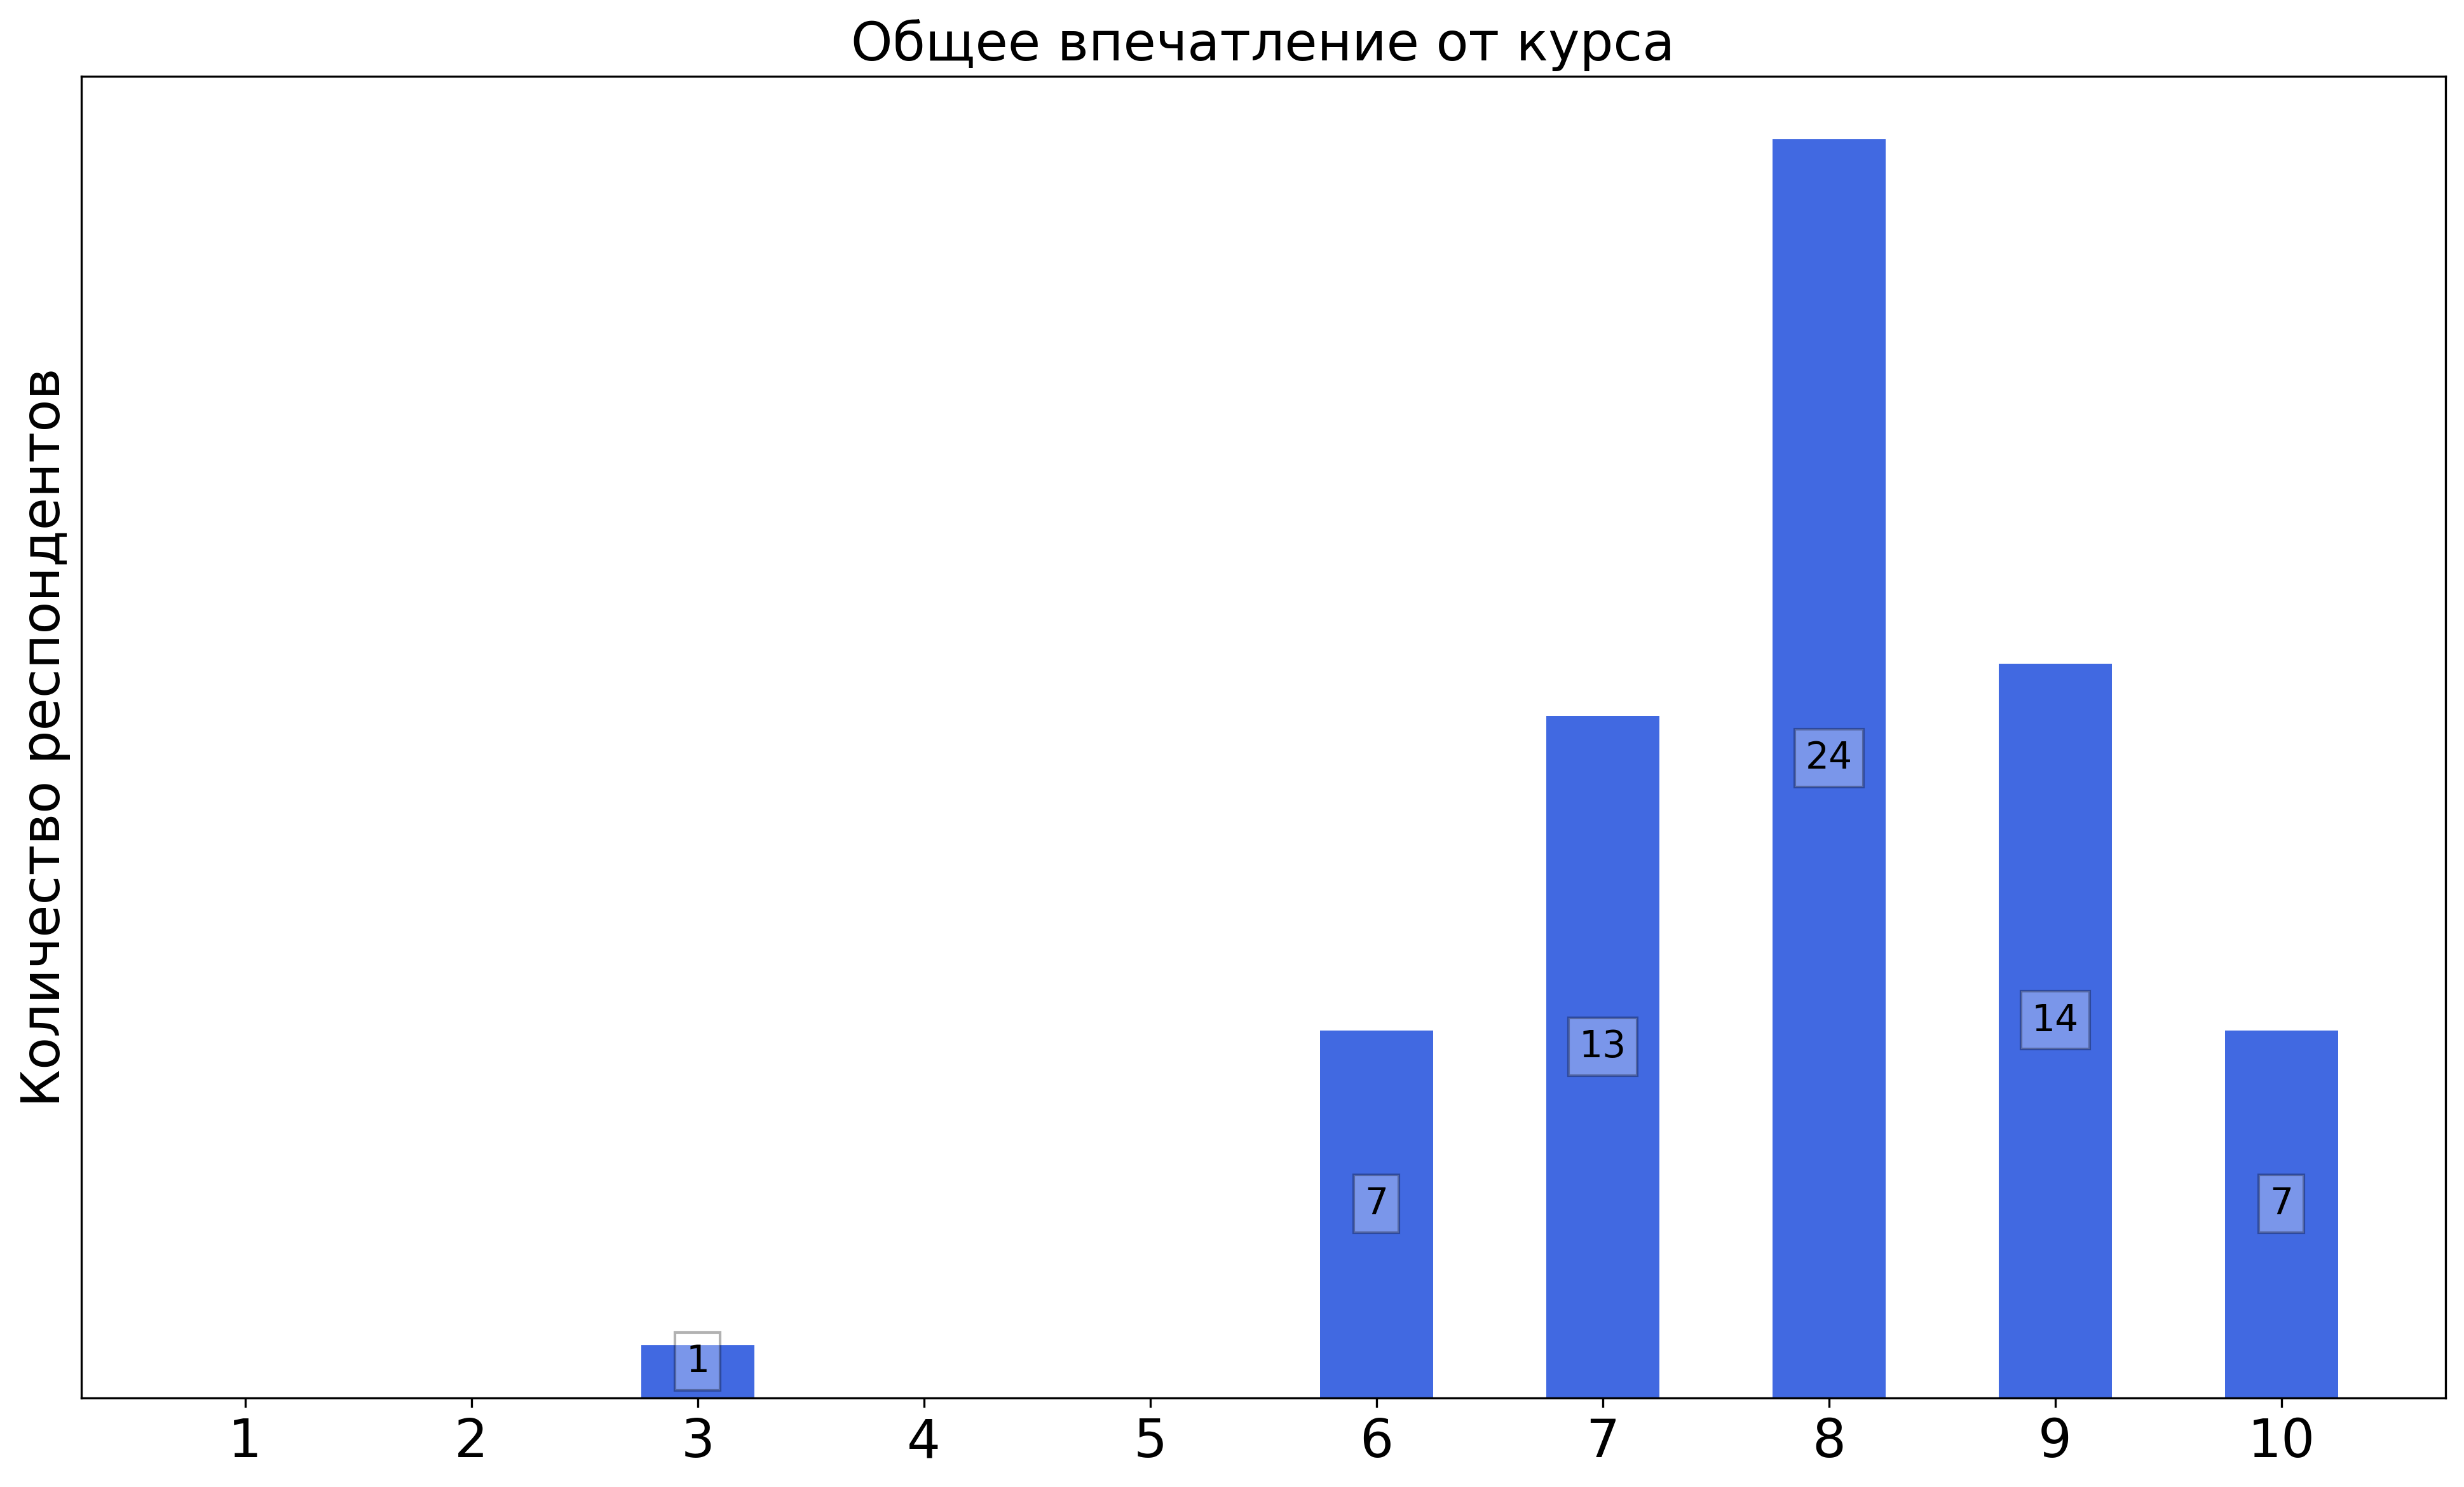
\includegraphics[width=\textwidth]{images/1 course/Математический анализ/general-0.png}
			\end{subfigure}
			\begin{subfigure}[b]{0.45\textwidth}
				\centering
				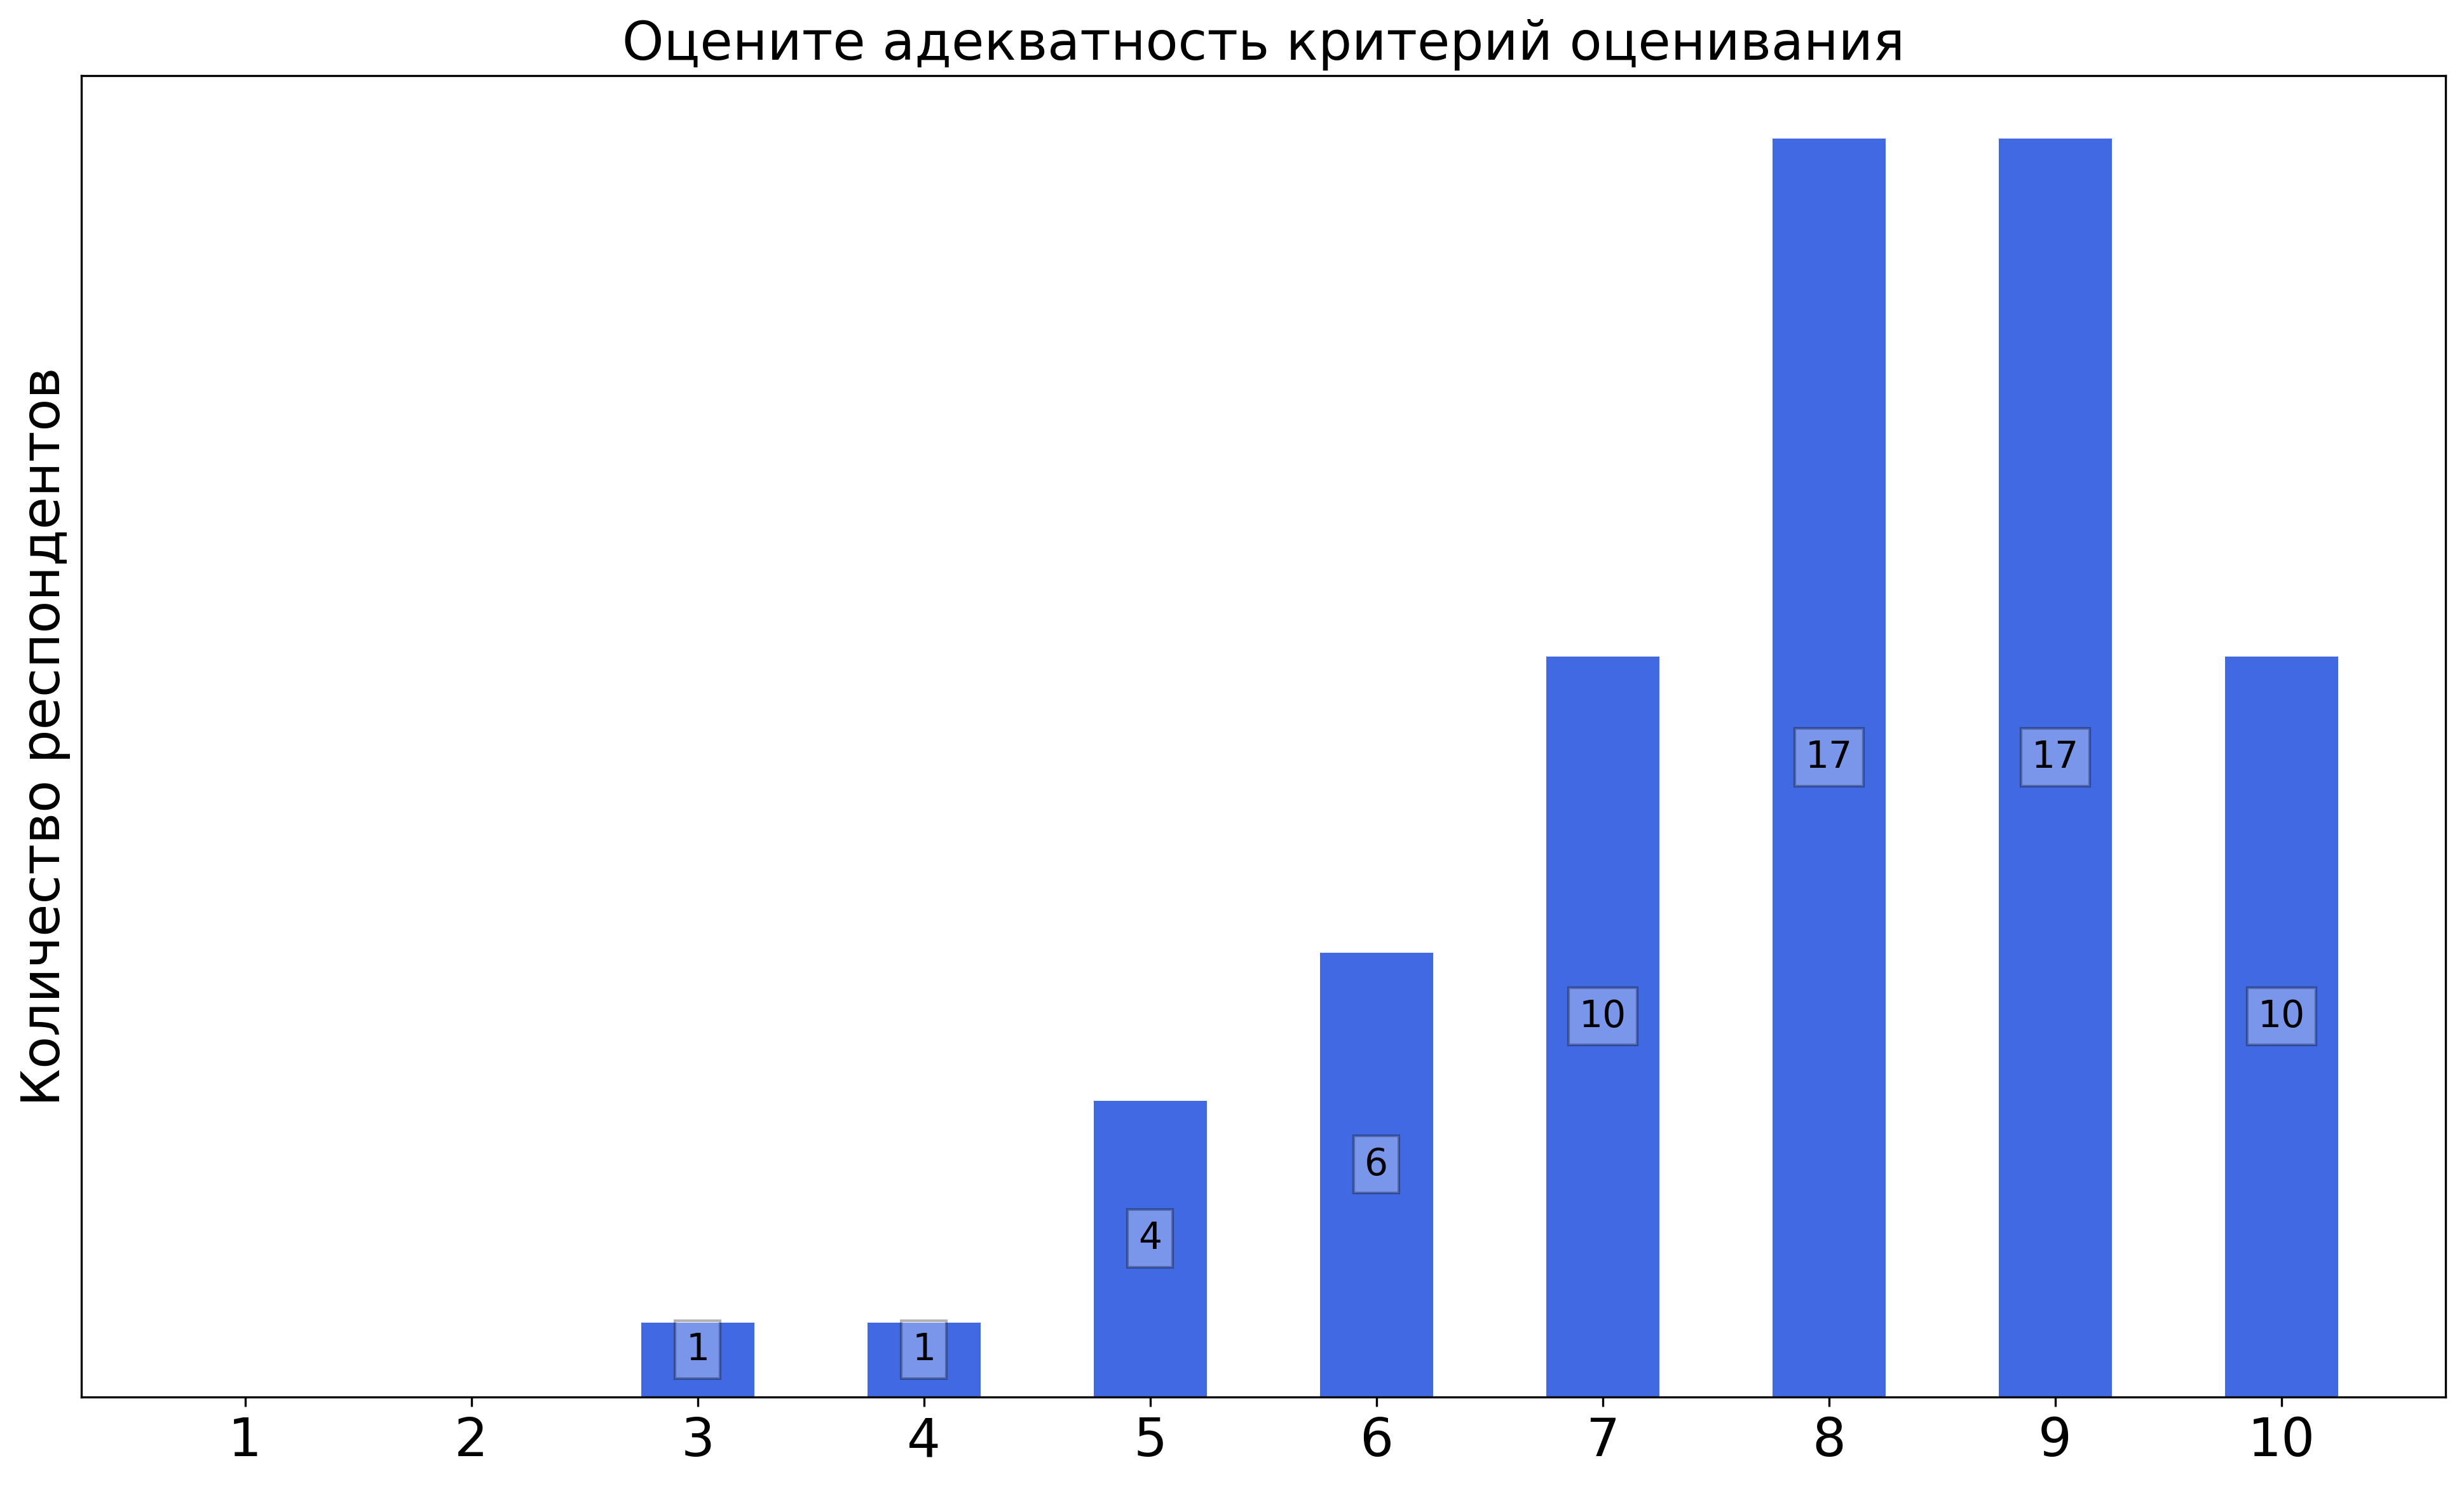
\includegraphics[width=\textwidth]{images/1 course/Математический анализ/general-1.png}
			\end{subfigure}	
		\end{figure}

	\subsubsection{Материалы, использумые респондентами при изучении курса}

		\begin{figure}[H]
			\centering
			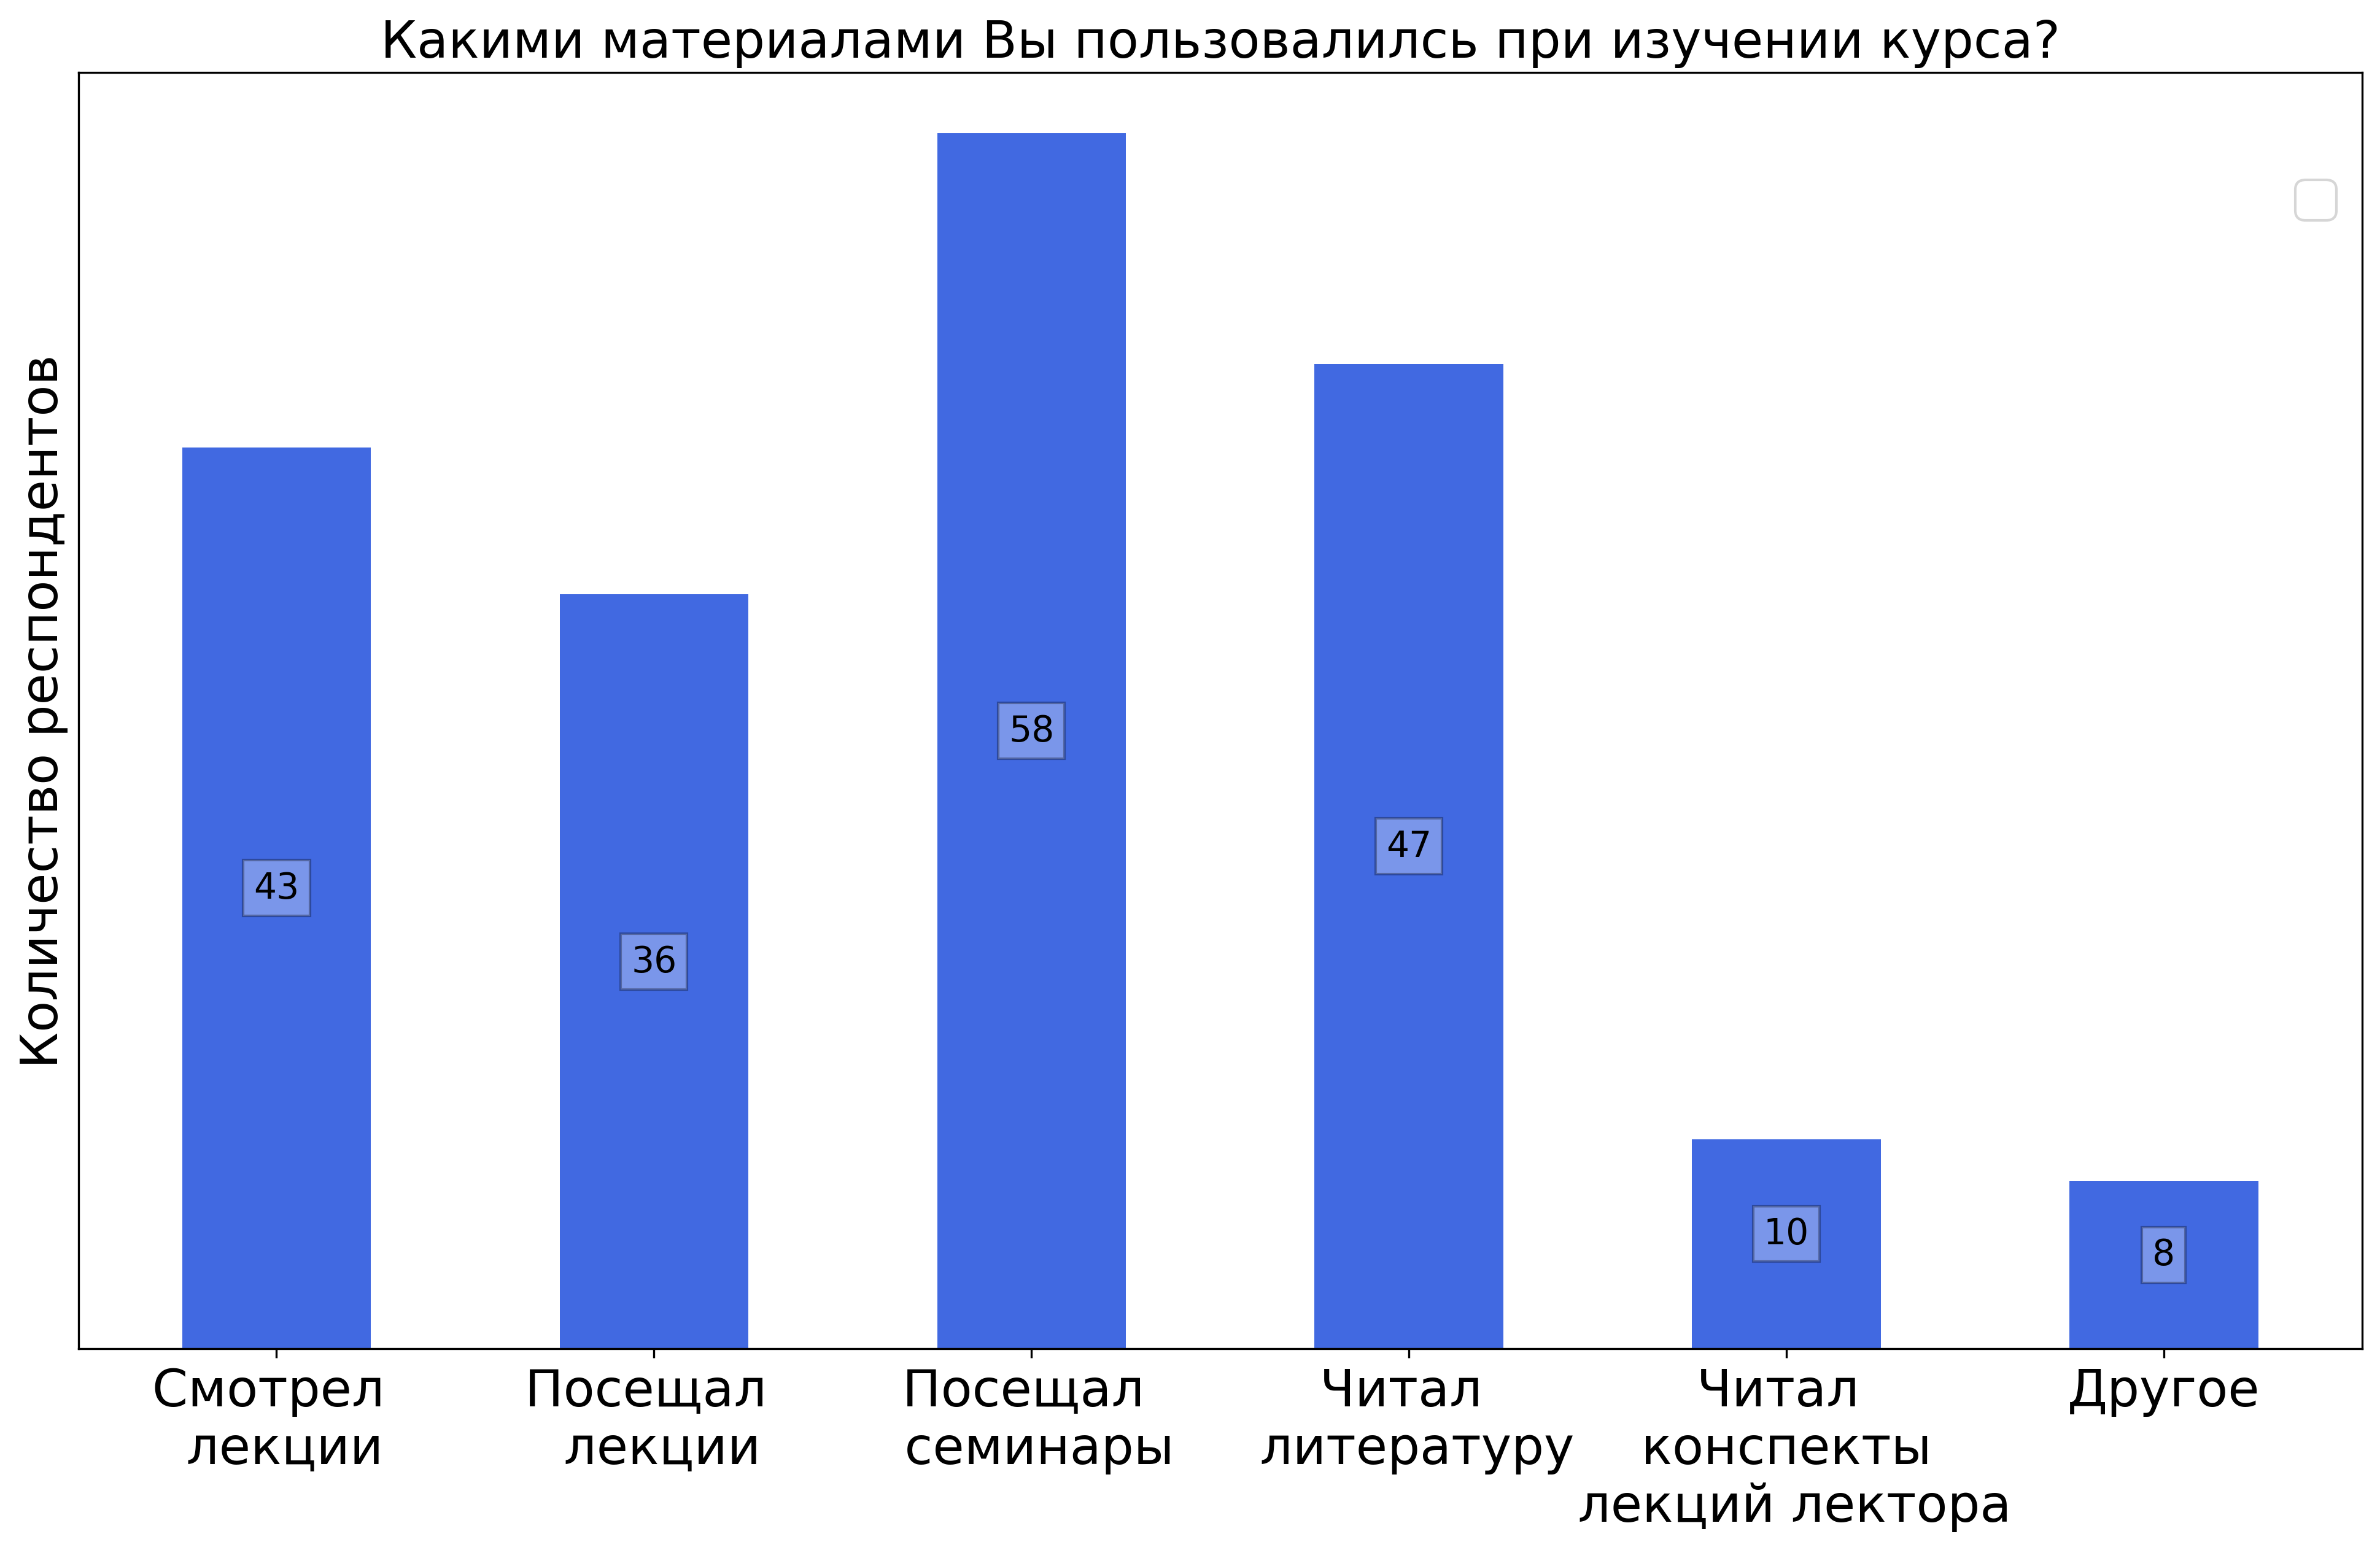
\includegraphics[width = 0.45\textwidth]{images/1 course/Математический анализ/materials.png}
		\end{figure}

		\textit{В качестве других источников информации студенты указали:} 
		\begin{itemize}
			\item материалы из интернета;
			\item лекции Сергея Жесткова.
		\end{itemize}

	\subsubsection{Отзыв студентов о лекциях. Лектор: Знаменская Л.Н.}

		\begin{figure}[H]
			\centering
			\begin{subfigure}[b]{0.45\textwidth}
				\centering
				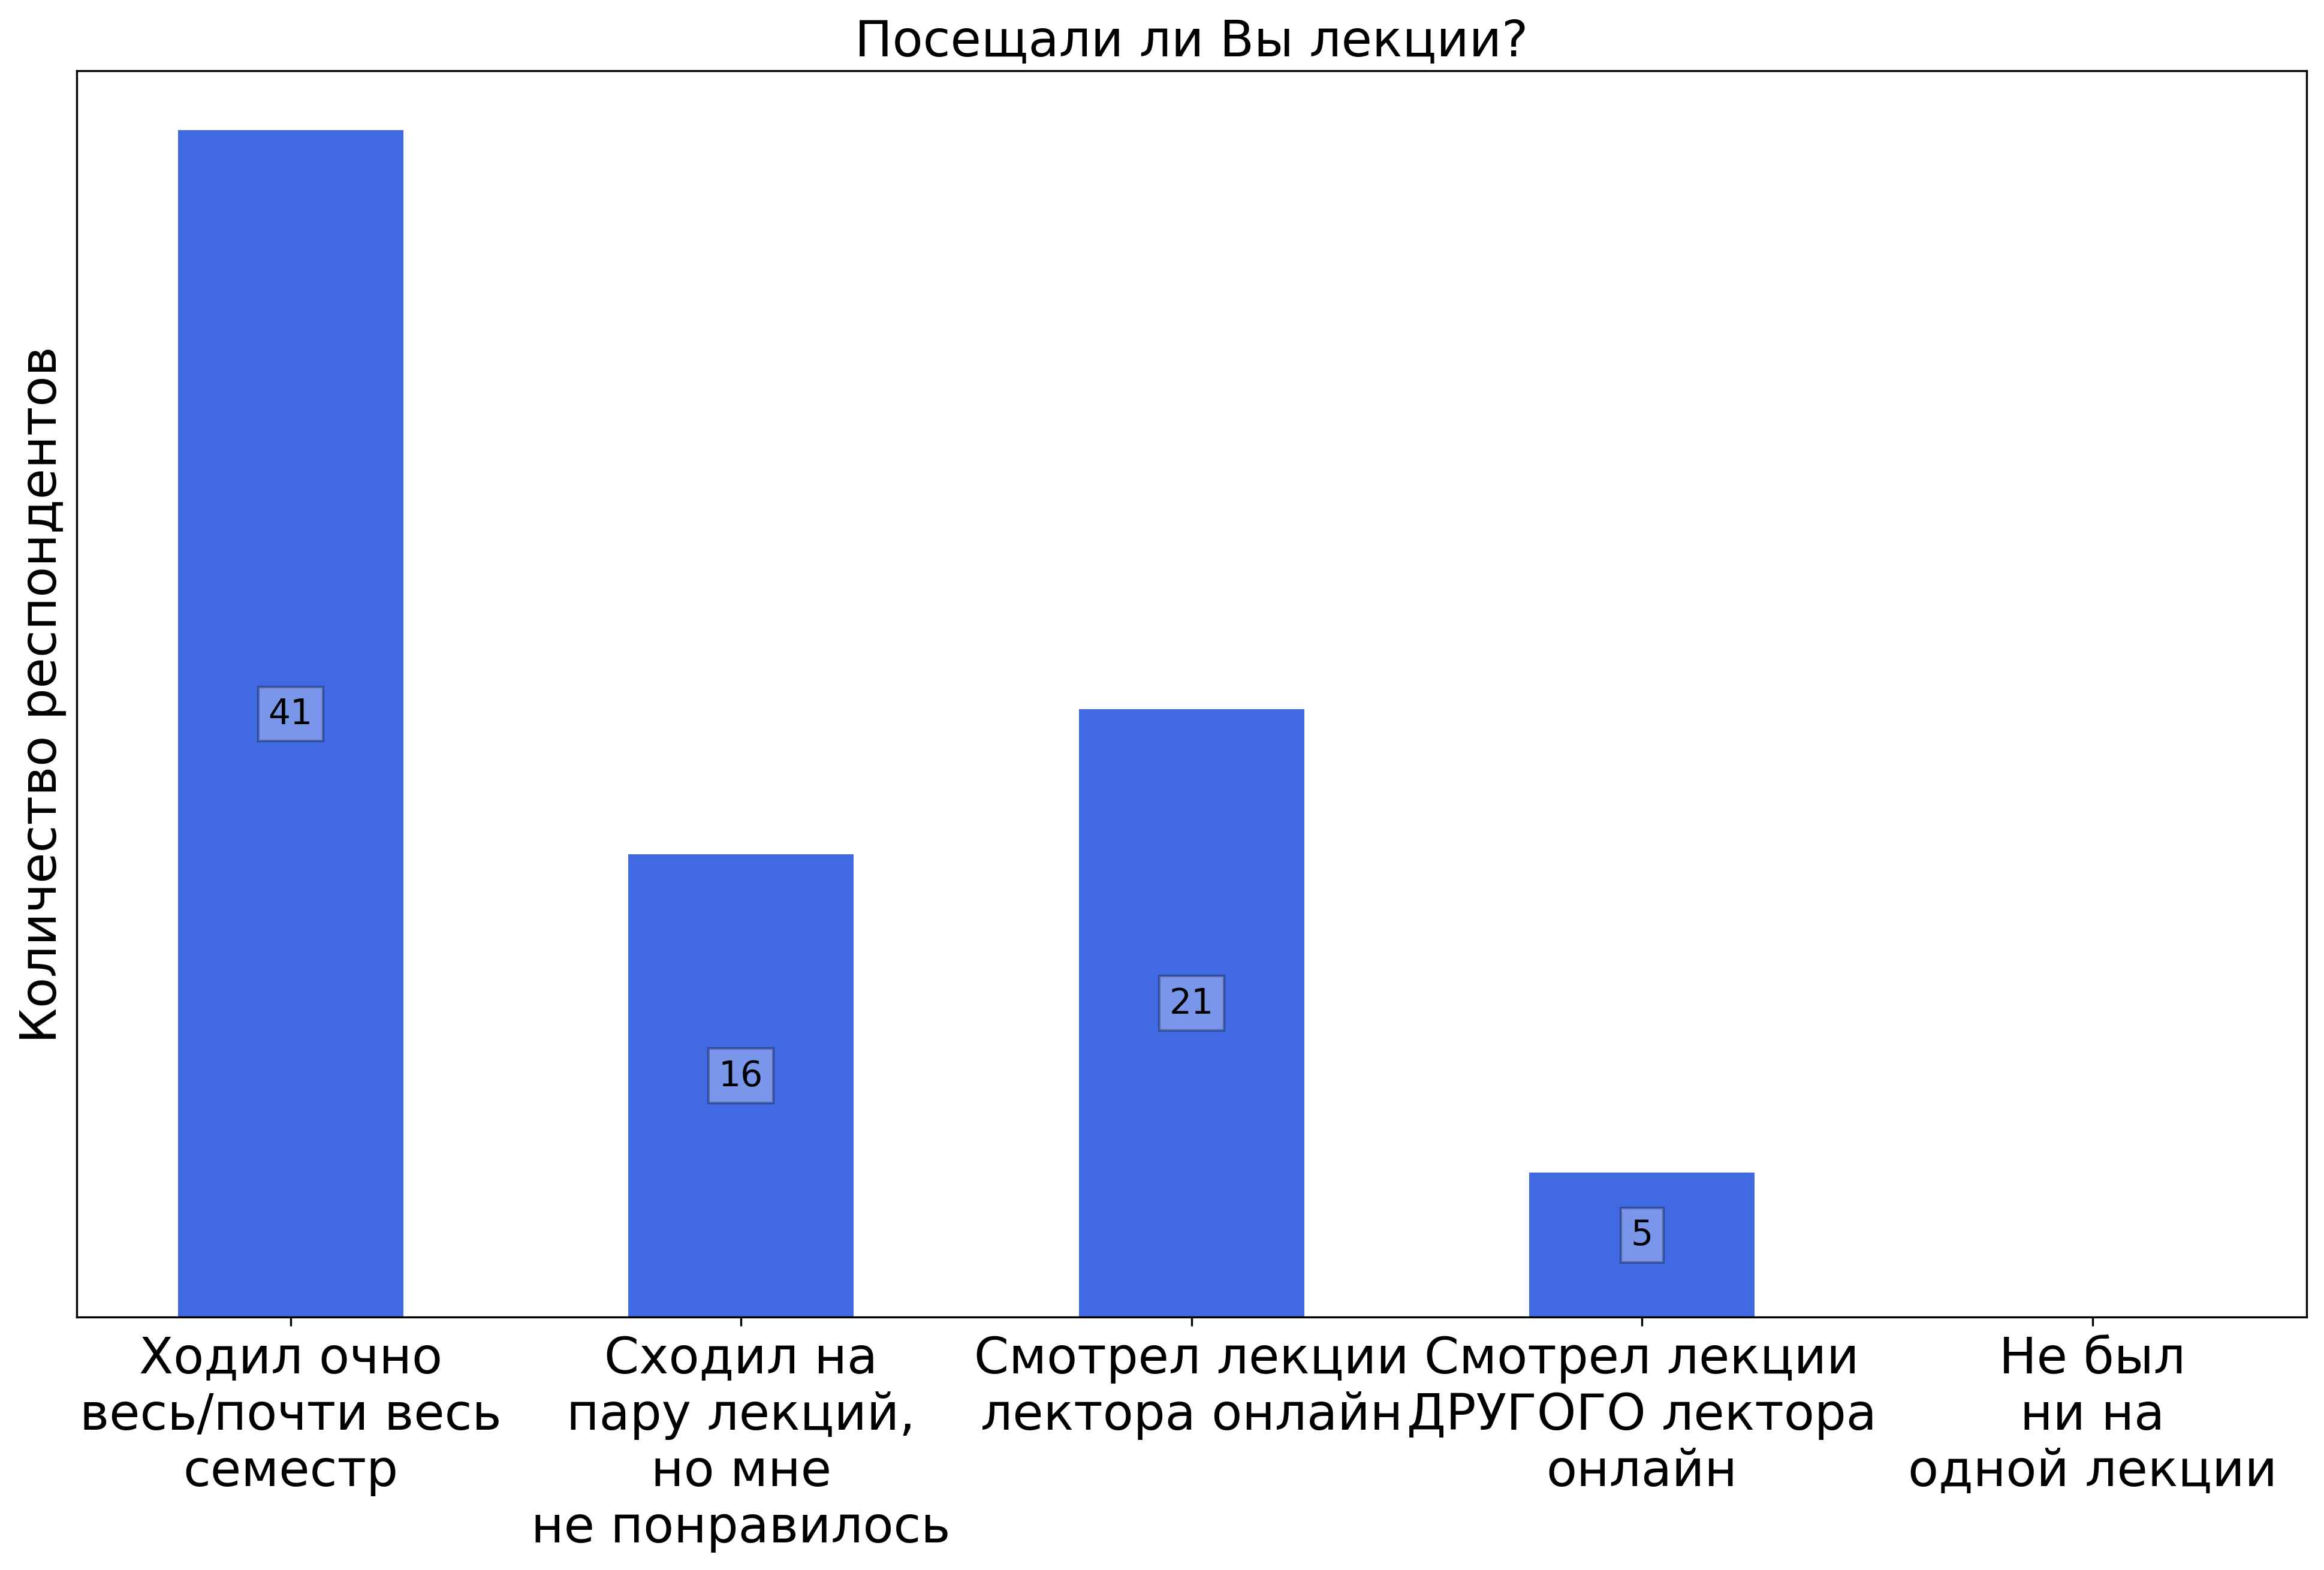
\includegraphics[width=\textwidth]{images/1 course/Математический анализ/lecturer-questions-Знаменская Л.Н.-0.png}
			\end{subfigure}
			\begin{subfigure}[b]{0.45\textwidth}
				\centering
				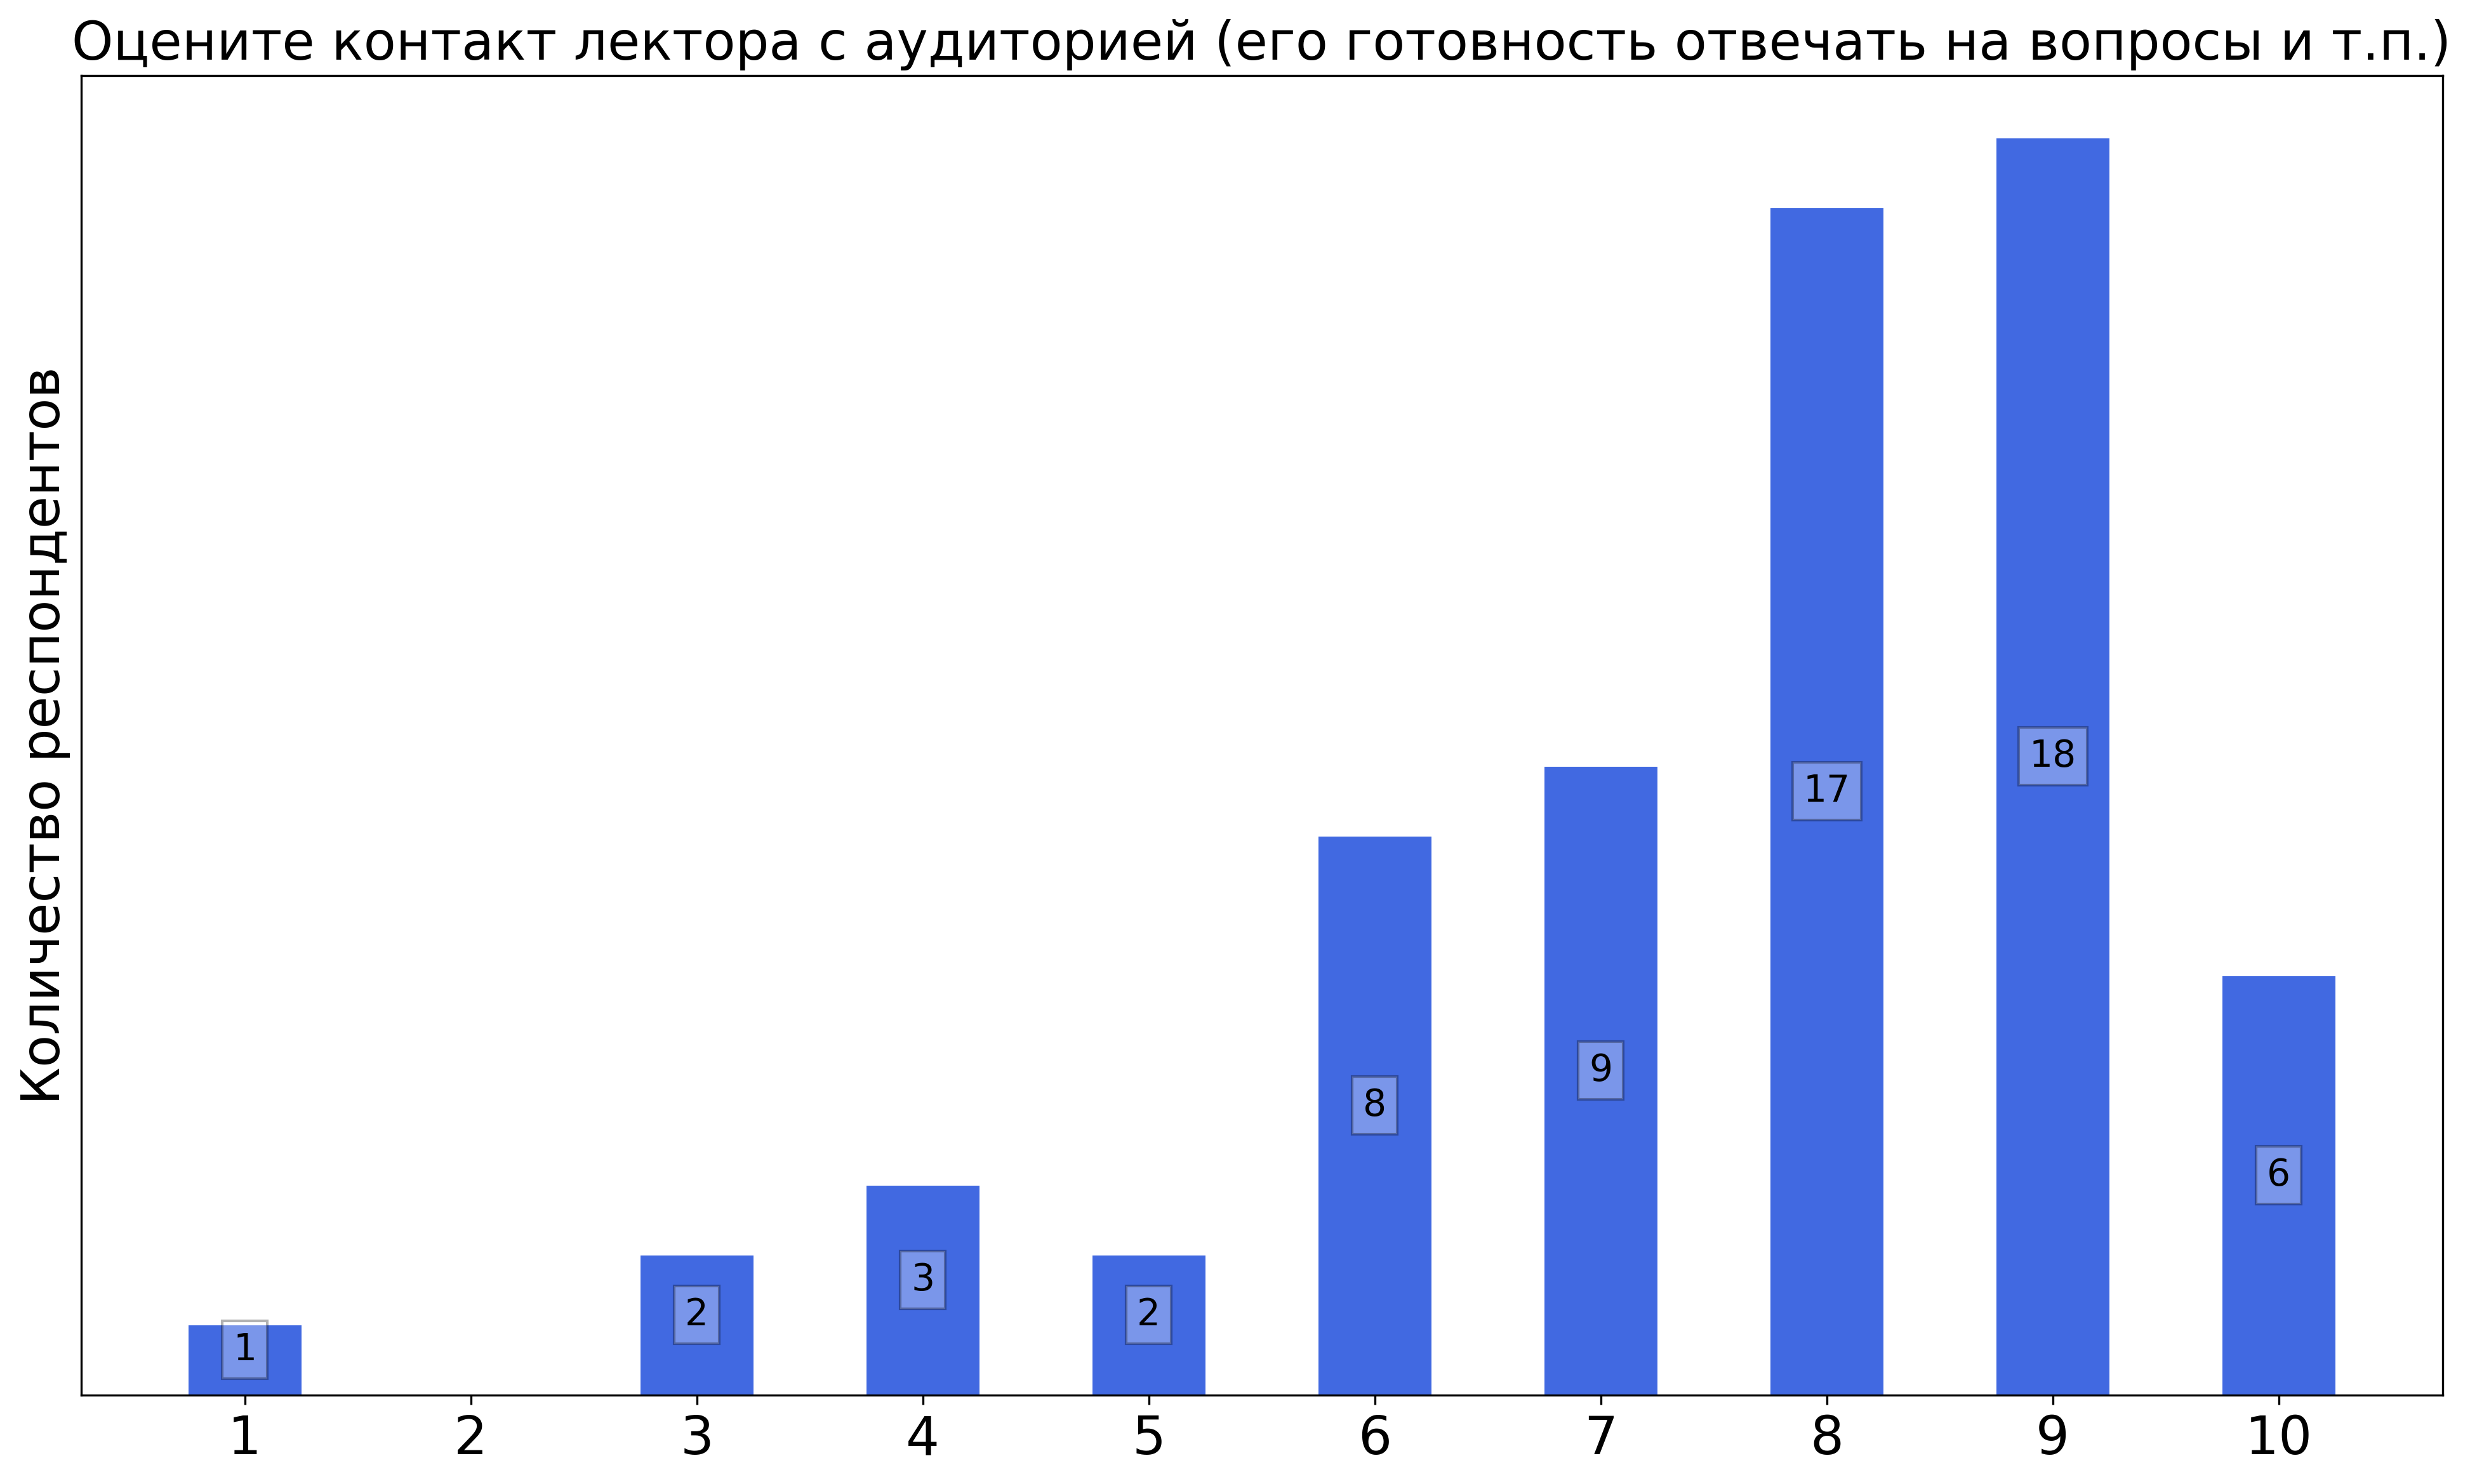
\includegraphics[width=\textwidth]{images/1 course/Математический анализ/lecturer-marks-Знаменская Л.Н.-0.png}
			\end{subfigure}
			\begin{subfigure}[b]{0.45\textwidth}
				\centering
				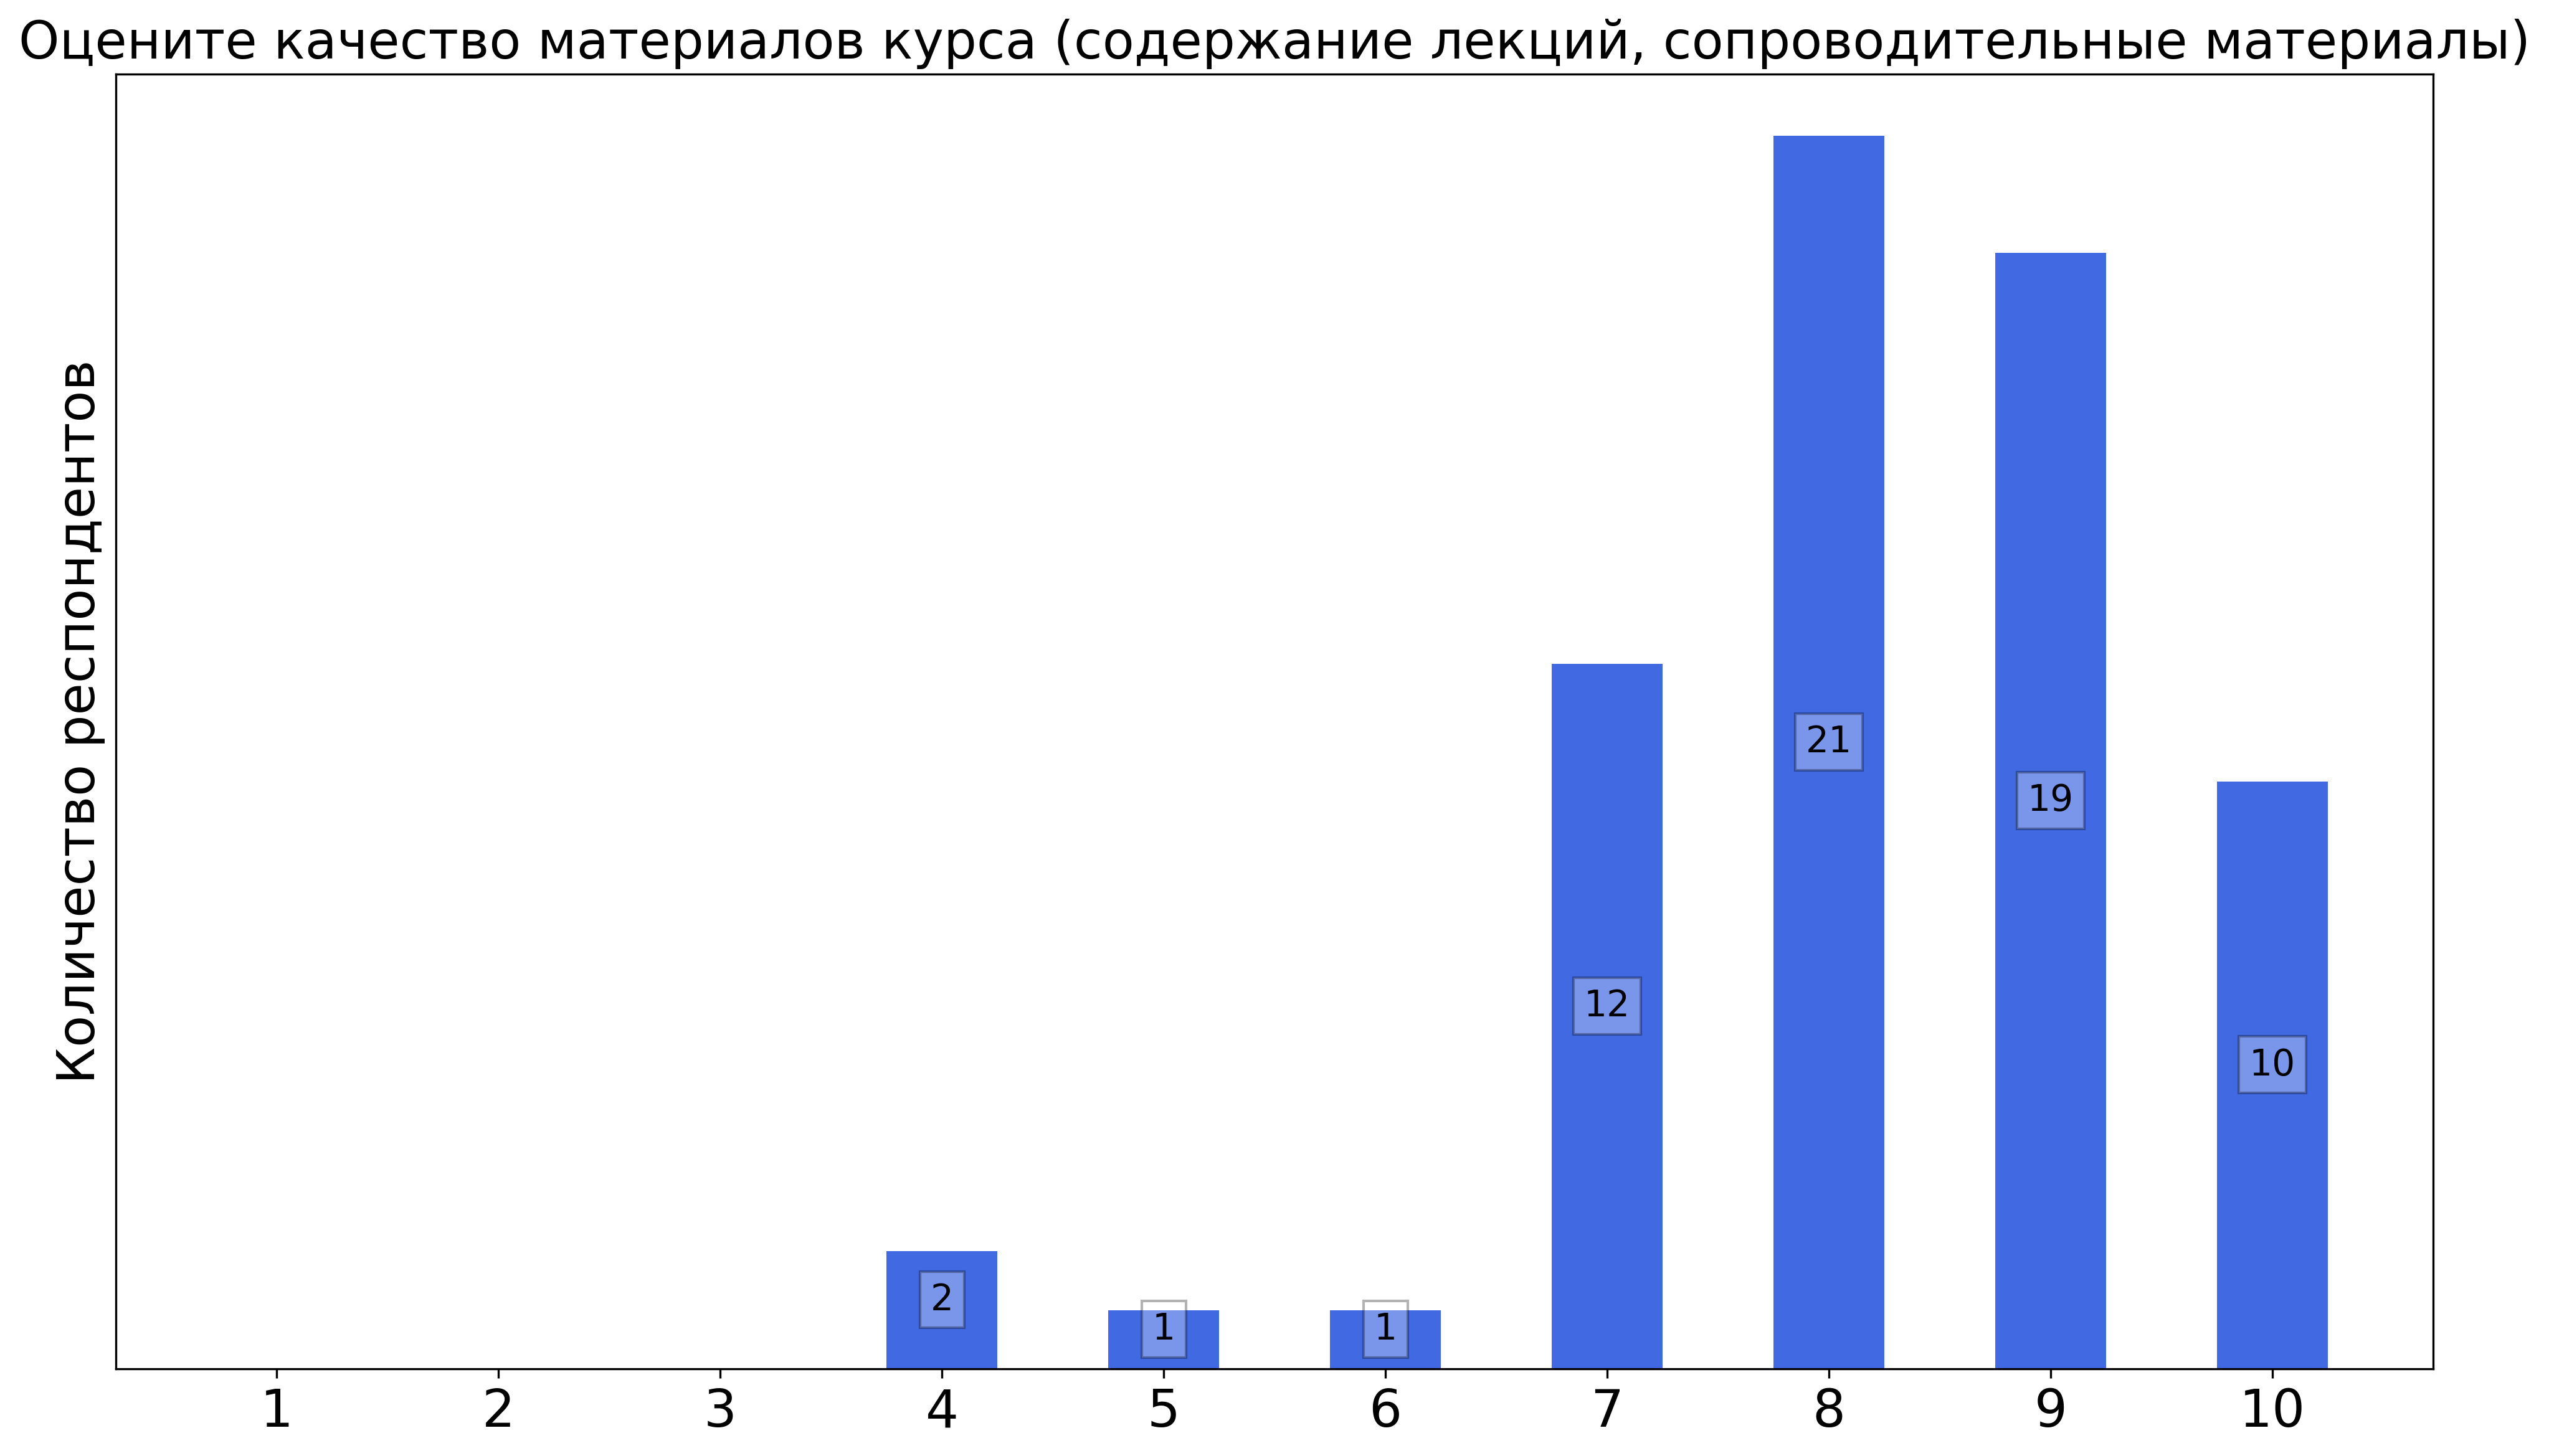
\includegraphics[width=\textwidth]{images/1 course/Математический анализ/lecturer-marks-Знаменская Л.Н.-1.png}
			\end{subfigure}
			\begin{subfigure}[b]{0.45\textwidth}
				\centering
				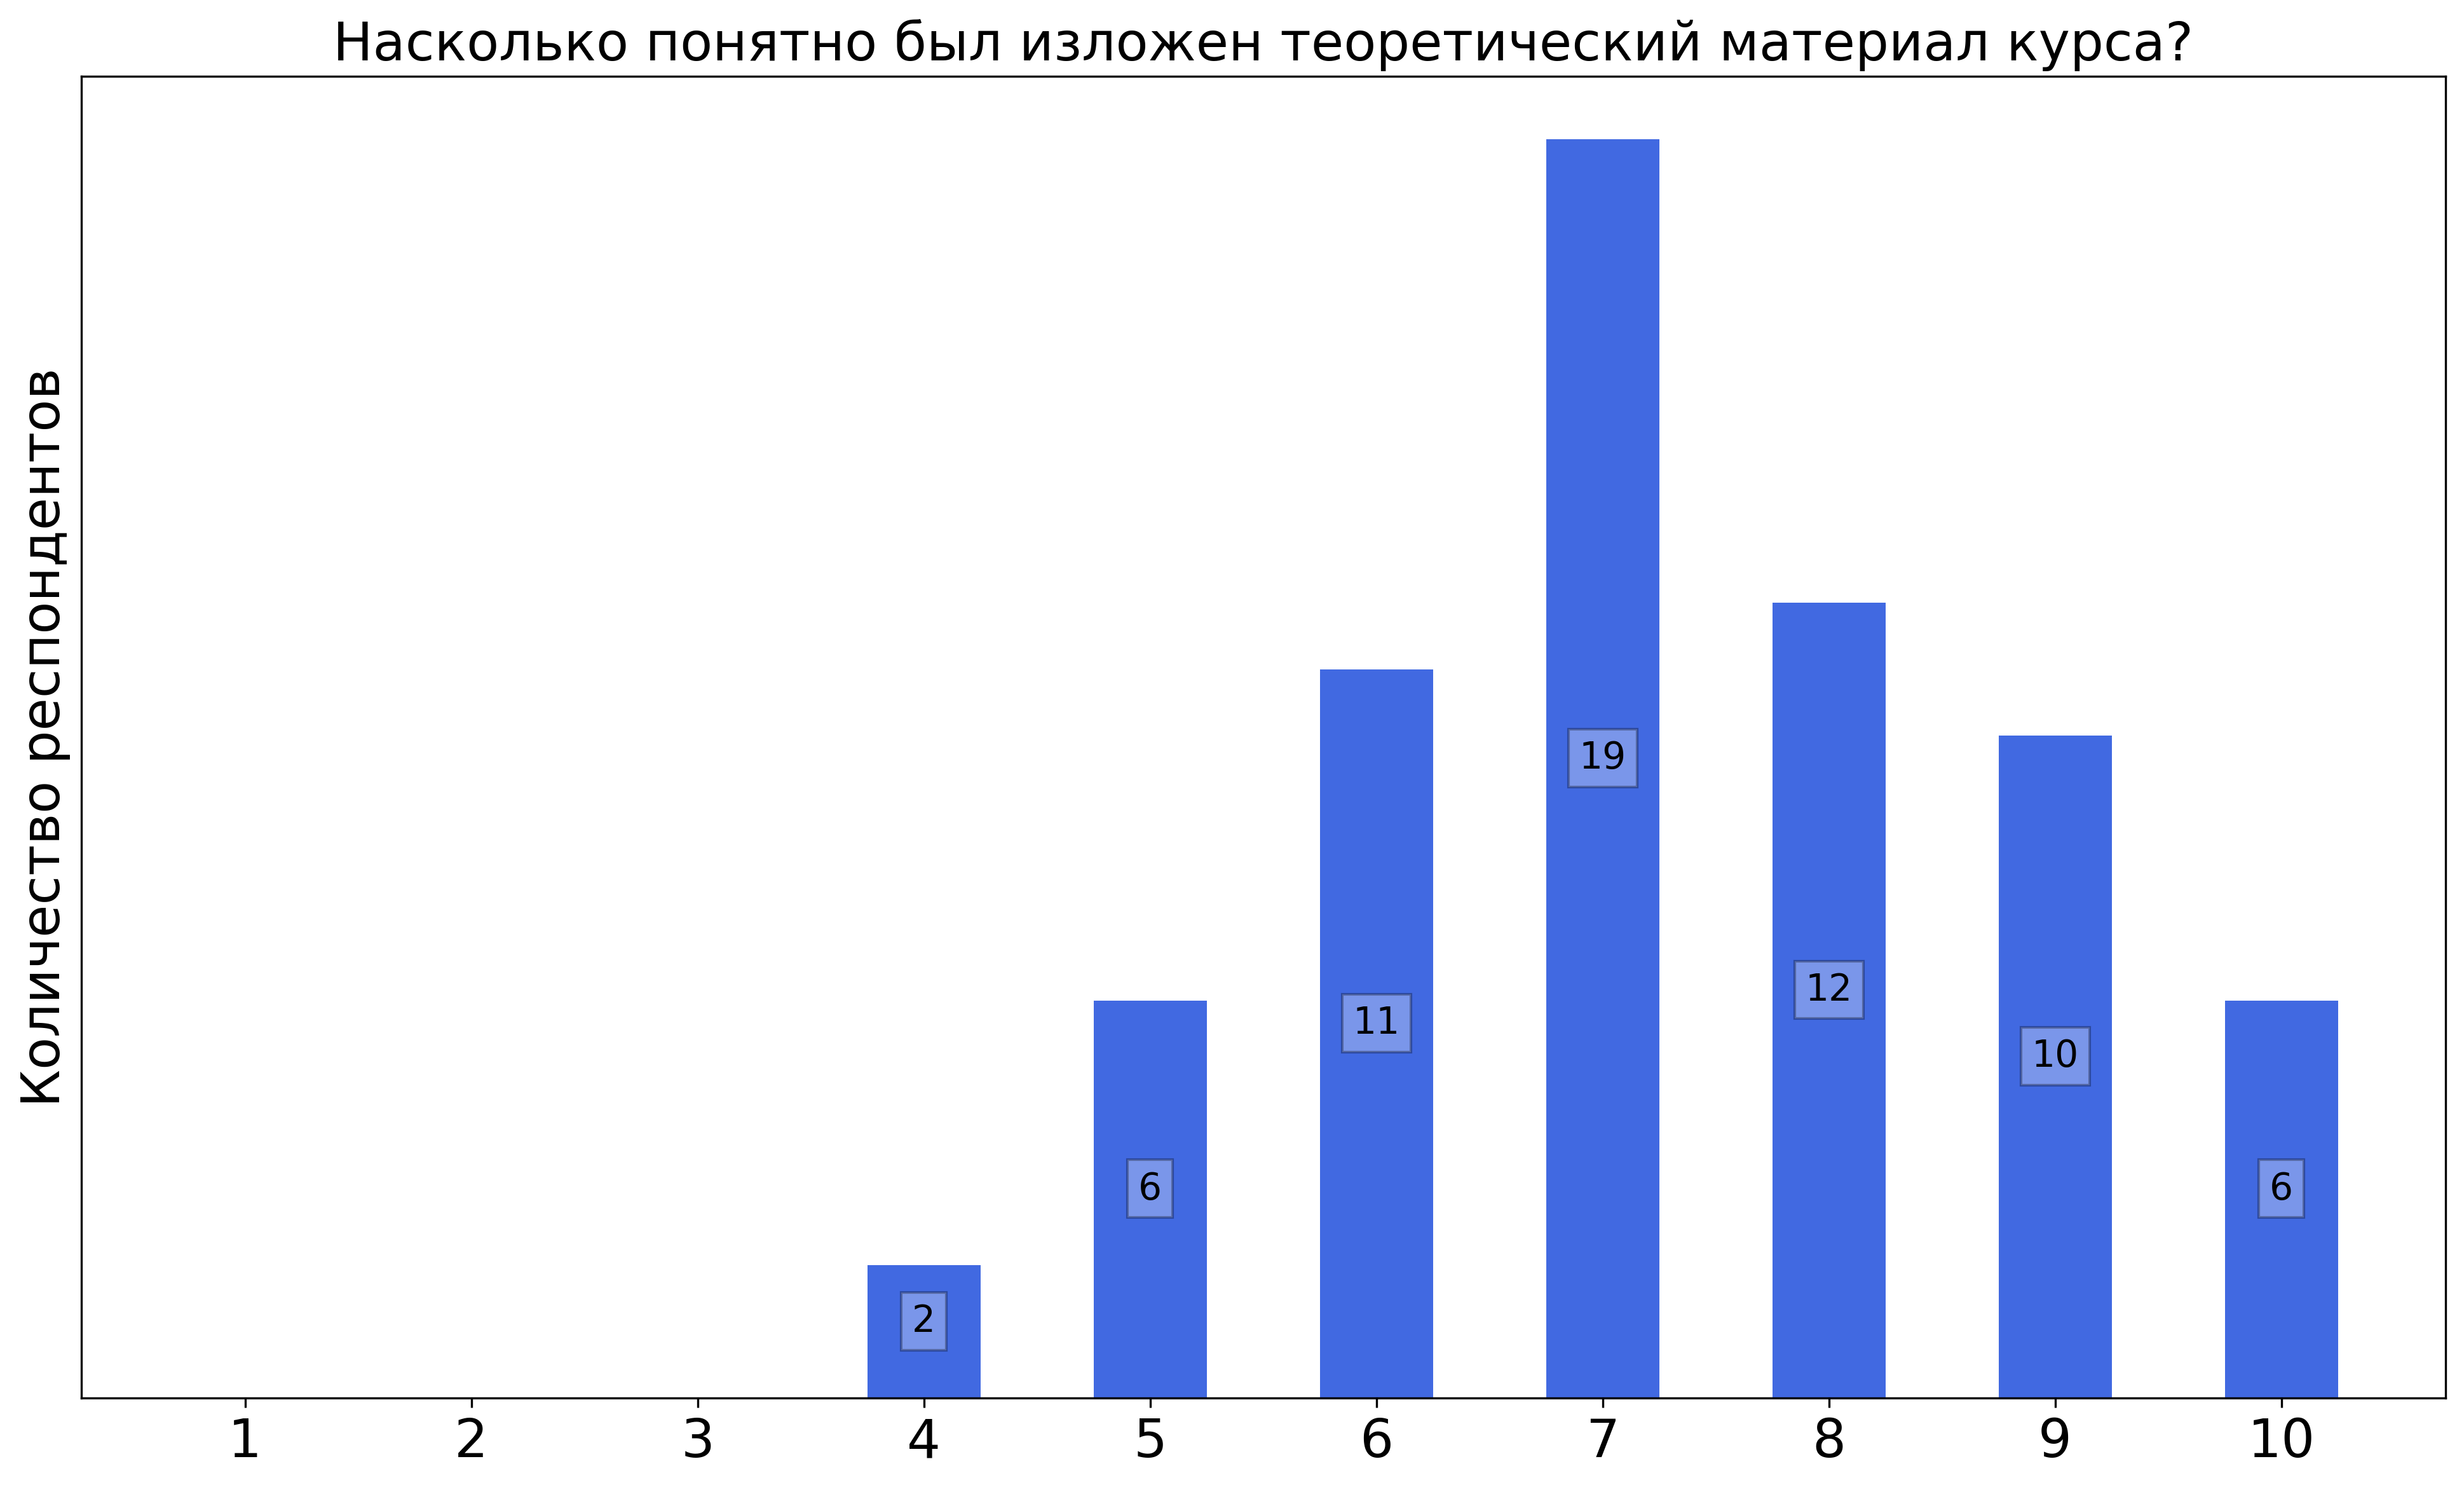
\includegraphics[width=\textwidth]{images/1 course/Математический анализ/lecturer-marks-Знаменская Л.Н.-2.png}
			\end{subfigure}	
			\begin{subfigure}[b]{0.45\textwidth}
				\centering
				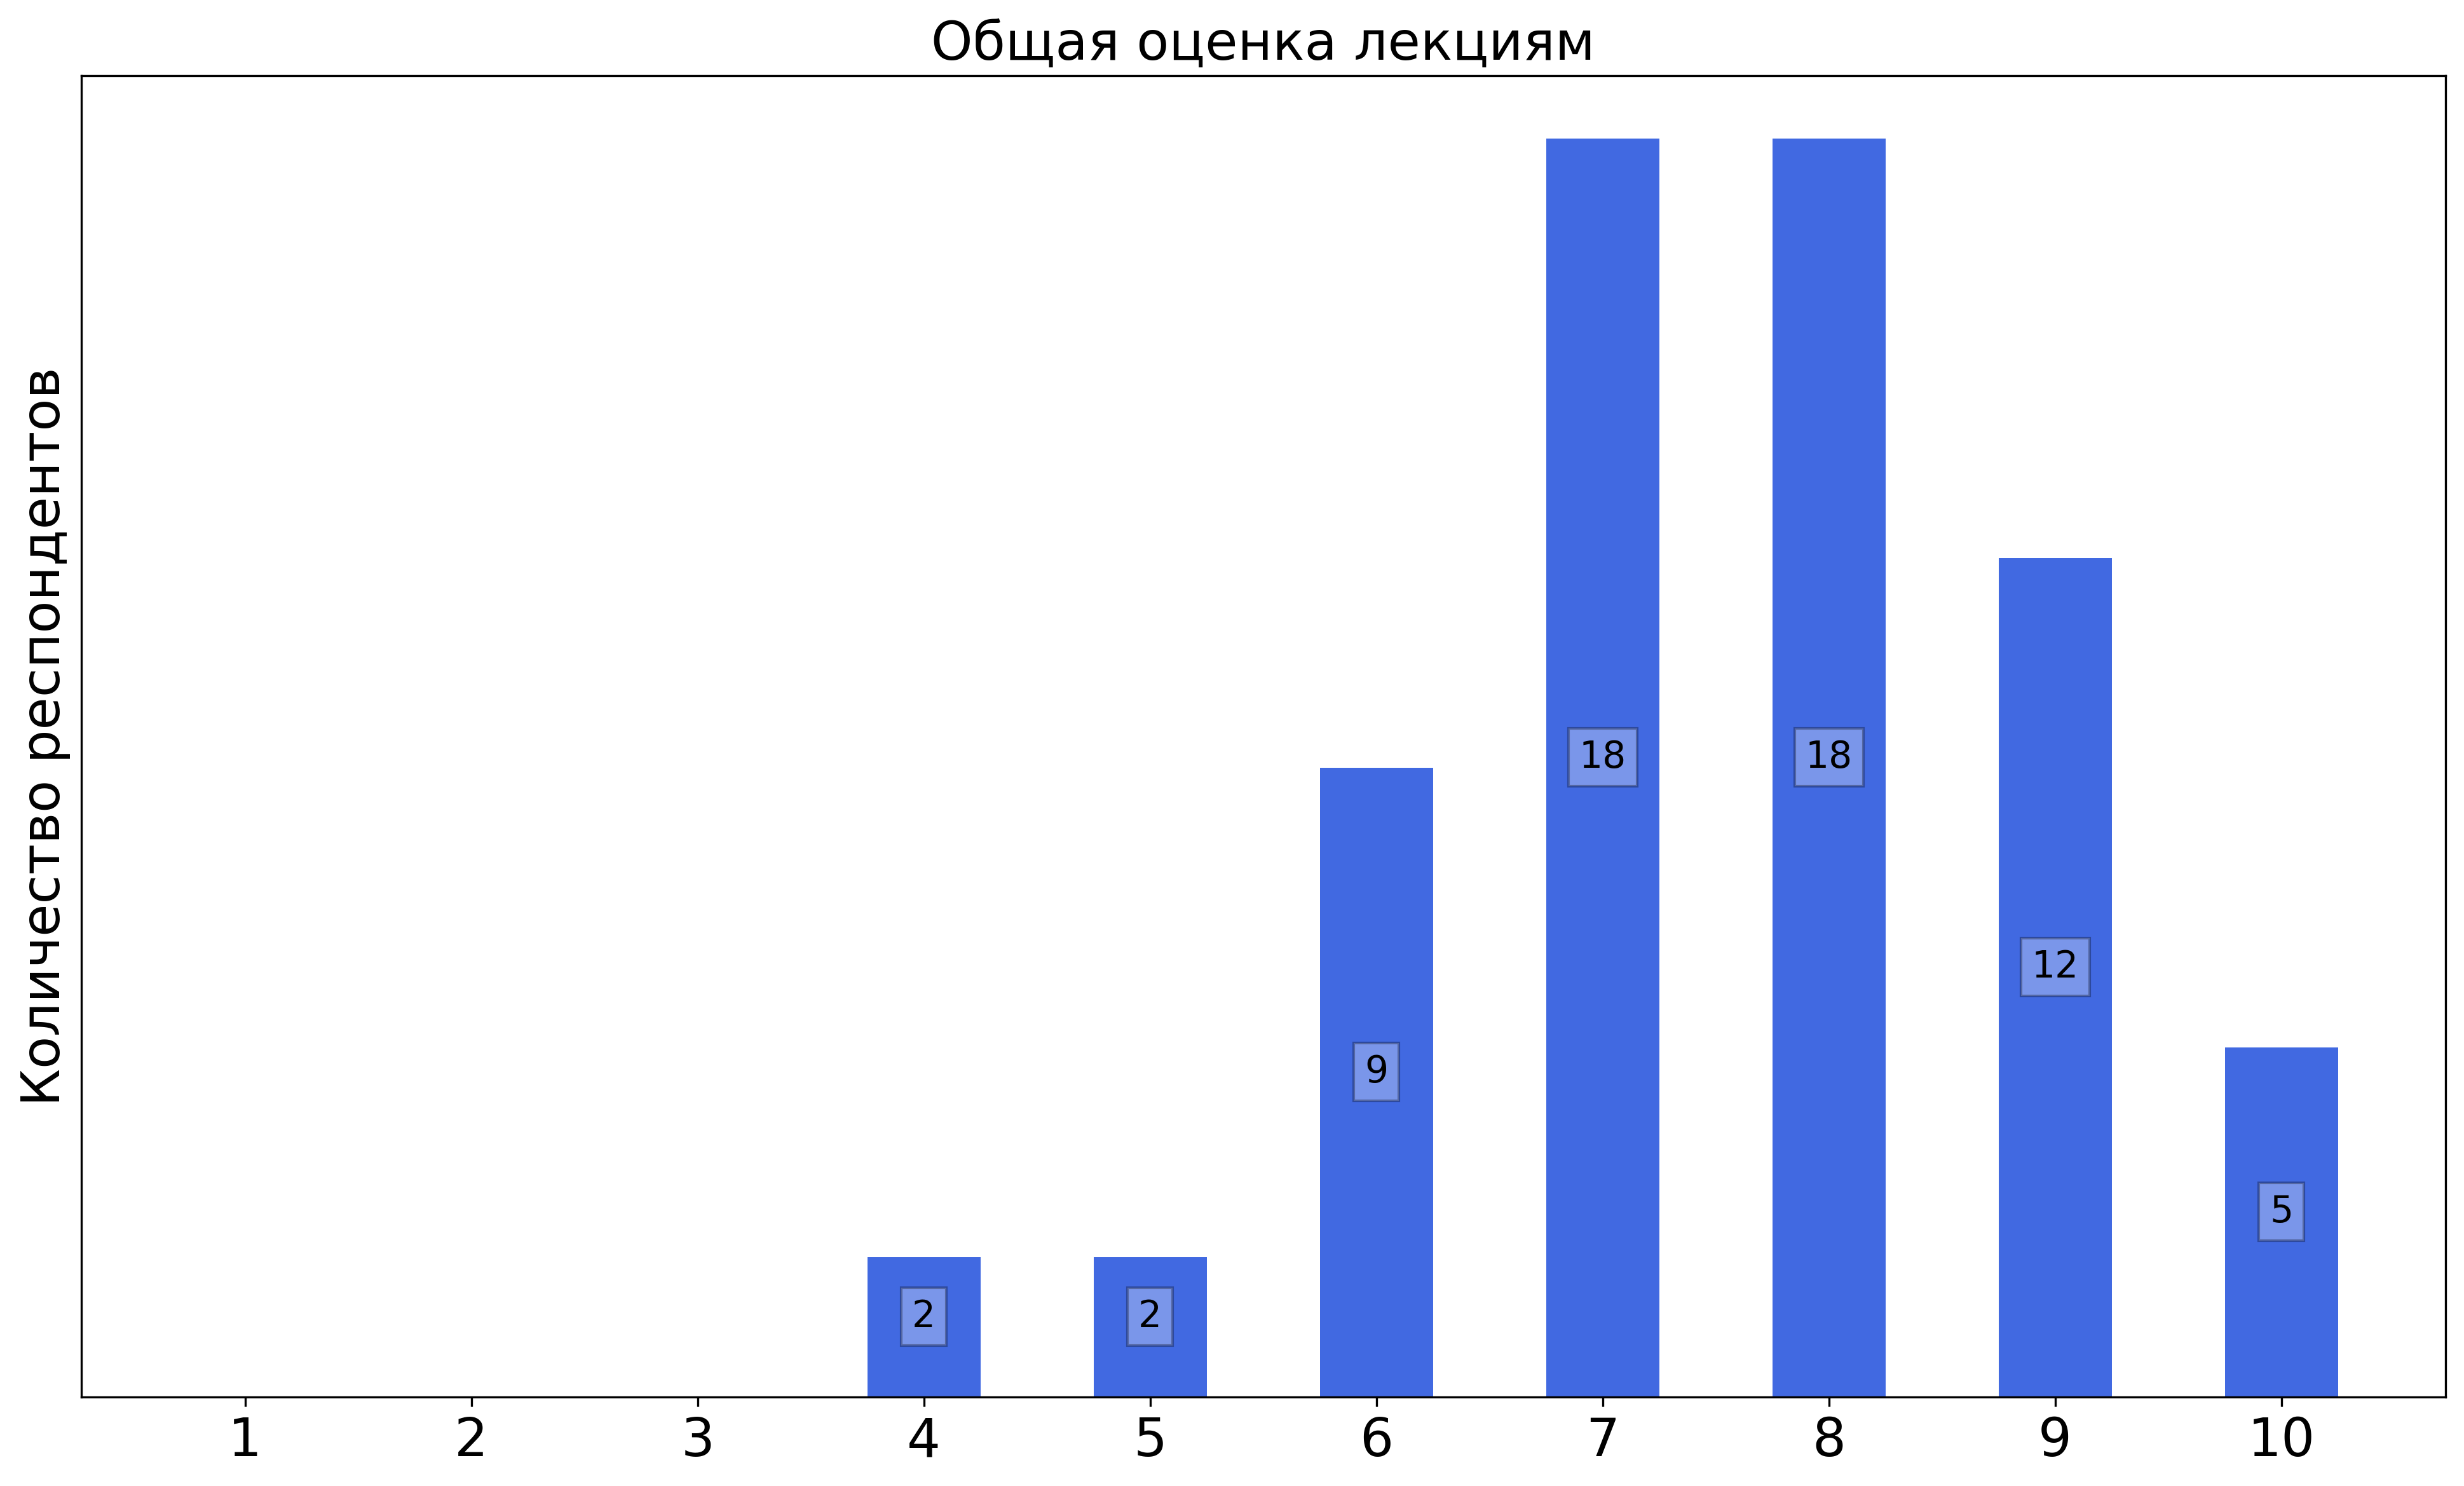
\includegraphics[width=\textwidth]{images/1 course/Математический анализ/lecturer-marks-Знаменская Л.Н.-3.png}
			\end{subfigure}
			\caption{Оценки респондентов о качестве преподавания лекций по курсу <<Введение в математический анализ>>}
		\end{figure}

		\textbf{Комментарии студентов о лекциях\protect\footnote{сохранены оригинальные орфография и пунктуация}}

		\begin{commentbox}
			Лекции по данному курсу в 1 семестре читались достаточно монотонно и скучно. Многие вещи, которые требовали доказательства, лектор не доказывала, а оставляла "в качестве упражнения". В результате приходилось полностью готовиться по книжке другого лектора, при этом не используя конспекты лекций совершенно. Кроме того, в очень многих доказательствах пропускались важные промежуточные действия, что добавляло еще большей непонятности доказательству. На вопросы от студентов лектор отвечает не очень охотно. Больше чем уд4 поставить не могу.
		\end{commentbox}

		\begin{commentbox}
			Материал рассказывается довольно быстро, тяжело одновременно осознавать что происходит и записывать. Очень выручала книга, дублирующая лекции.
		\end{commentbox}

		\begin{commentbox}
			Зачастую думает, что всем понятно, потому что ей понятно и очевидно, но это не так)
		\end{commentbox}

		\begin{commentbox}
			В целом все замечательно, за одним  но: на устной сдаче как известно можно пойти к лектору, однако Людмила Николаевна группы из третьего захода не взяла (потому что после первого и второго уже много человек было), так что такие критерии выбора кто ей будет сдавать, а кто нет кажутся немного несправедливыми
		\end{commentbox}

		\begin{commentbox}
			Лектор материал знает хорошо, однако может не понравиться её подход
		\end{commentbox}

		\begin{commentbox}
			норм, но не всё очевидно, что очевидно знаменской
		\end{commentbox}

		\begin{commentbox}
			Хорошие лекции. В целом достаточно понятно и структурировано. Очень хорошо, что лекции прошлых лет полностью совпадают по содержанию, а так же хорошо, что есть учебник, повторяющий их.
		\end{commentbox}

		\begin{commentbox}
			Материал очень трудный для новичка. Невозможно понять с первого раза
		\end{commentbox}

		\begin{commentbox}
			Очень не хватает иллюстрирующих картинок
		\end{commentbox}

		\begin{commentbox}
			Иногда непонятно, но зато очень последовательно и всё, что нужно на экзамене, было рассказано на лекциях.
		\end{commentbox}

		\begin{commentbox}
			Лекции у Знаменской Л.Н. хорошо структурированы, что очень удобно при подготовке к экзаменам. Но с другой стороны, они немного самобытны - не всегда соотносятся с материалами других лекторов, поэтому иногда можно запутаться в определениях, формулировках теорем и тд, тп.
		\end{commentbox}

		\begin{commentbox}
			Лектор, кроме своих доказательств, ничего другого не принимает. Хотя у лектора бывают просто ужасные доказательства, просто взятые не понятно откуда. Хоть в мире и есть более простые доказательства и более понятные обществу, лектор их не будет засчитывать, тк они не его.
		\end{commentbox}

	\subsubsection{Отзыв студентов о семинарах. Семинарист: Загрядский О.А.}
		\begin{figure}[H]
			\centering
			\begin{subfigure}[b]{0.45\textwidth}
				\centering
				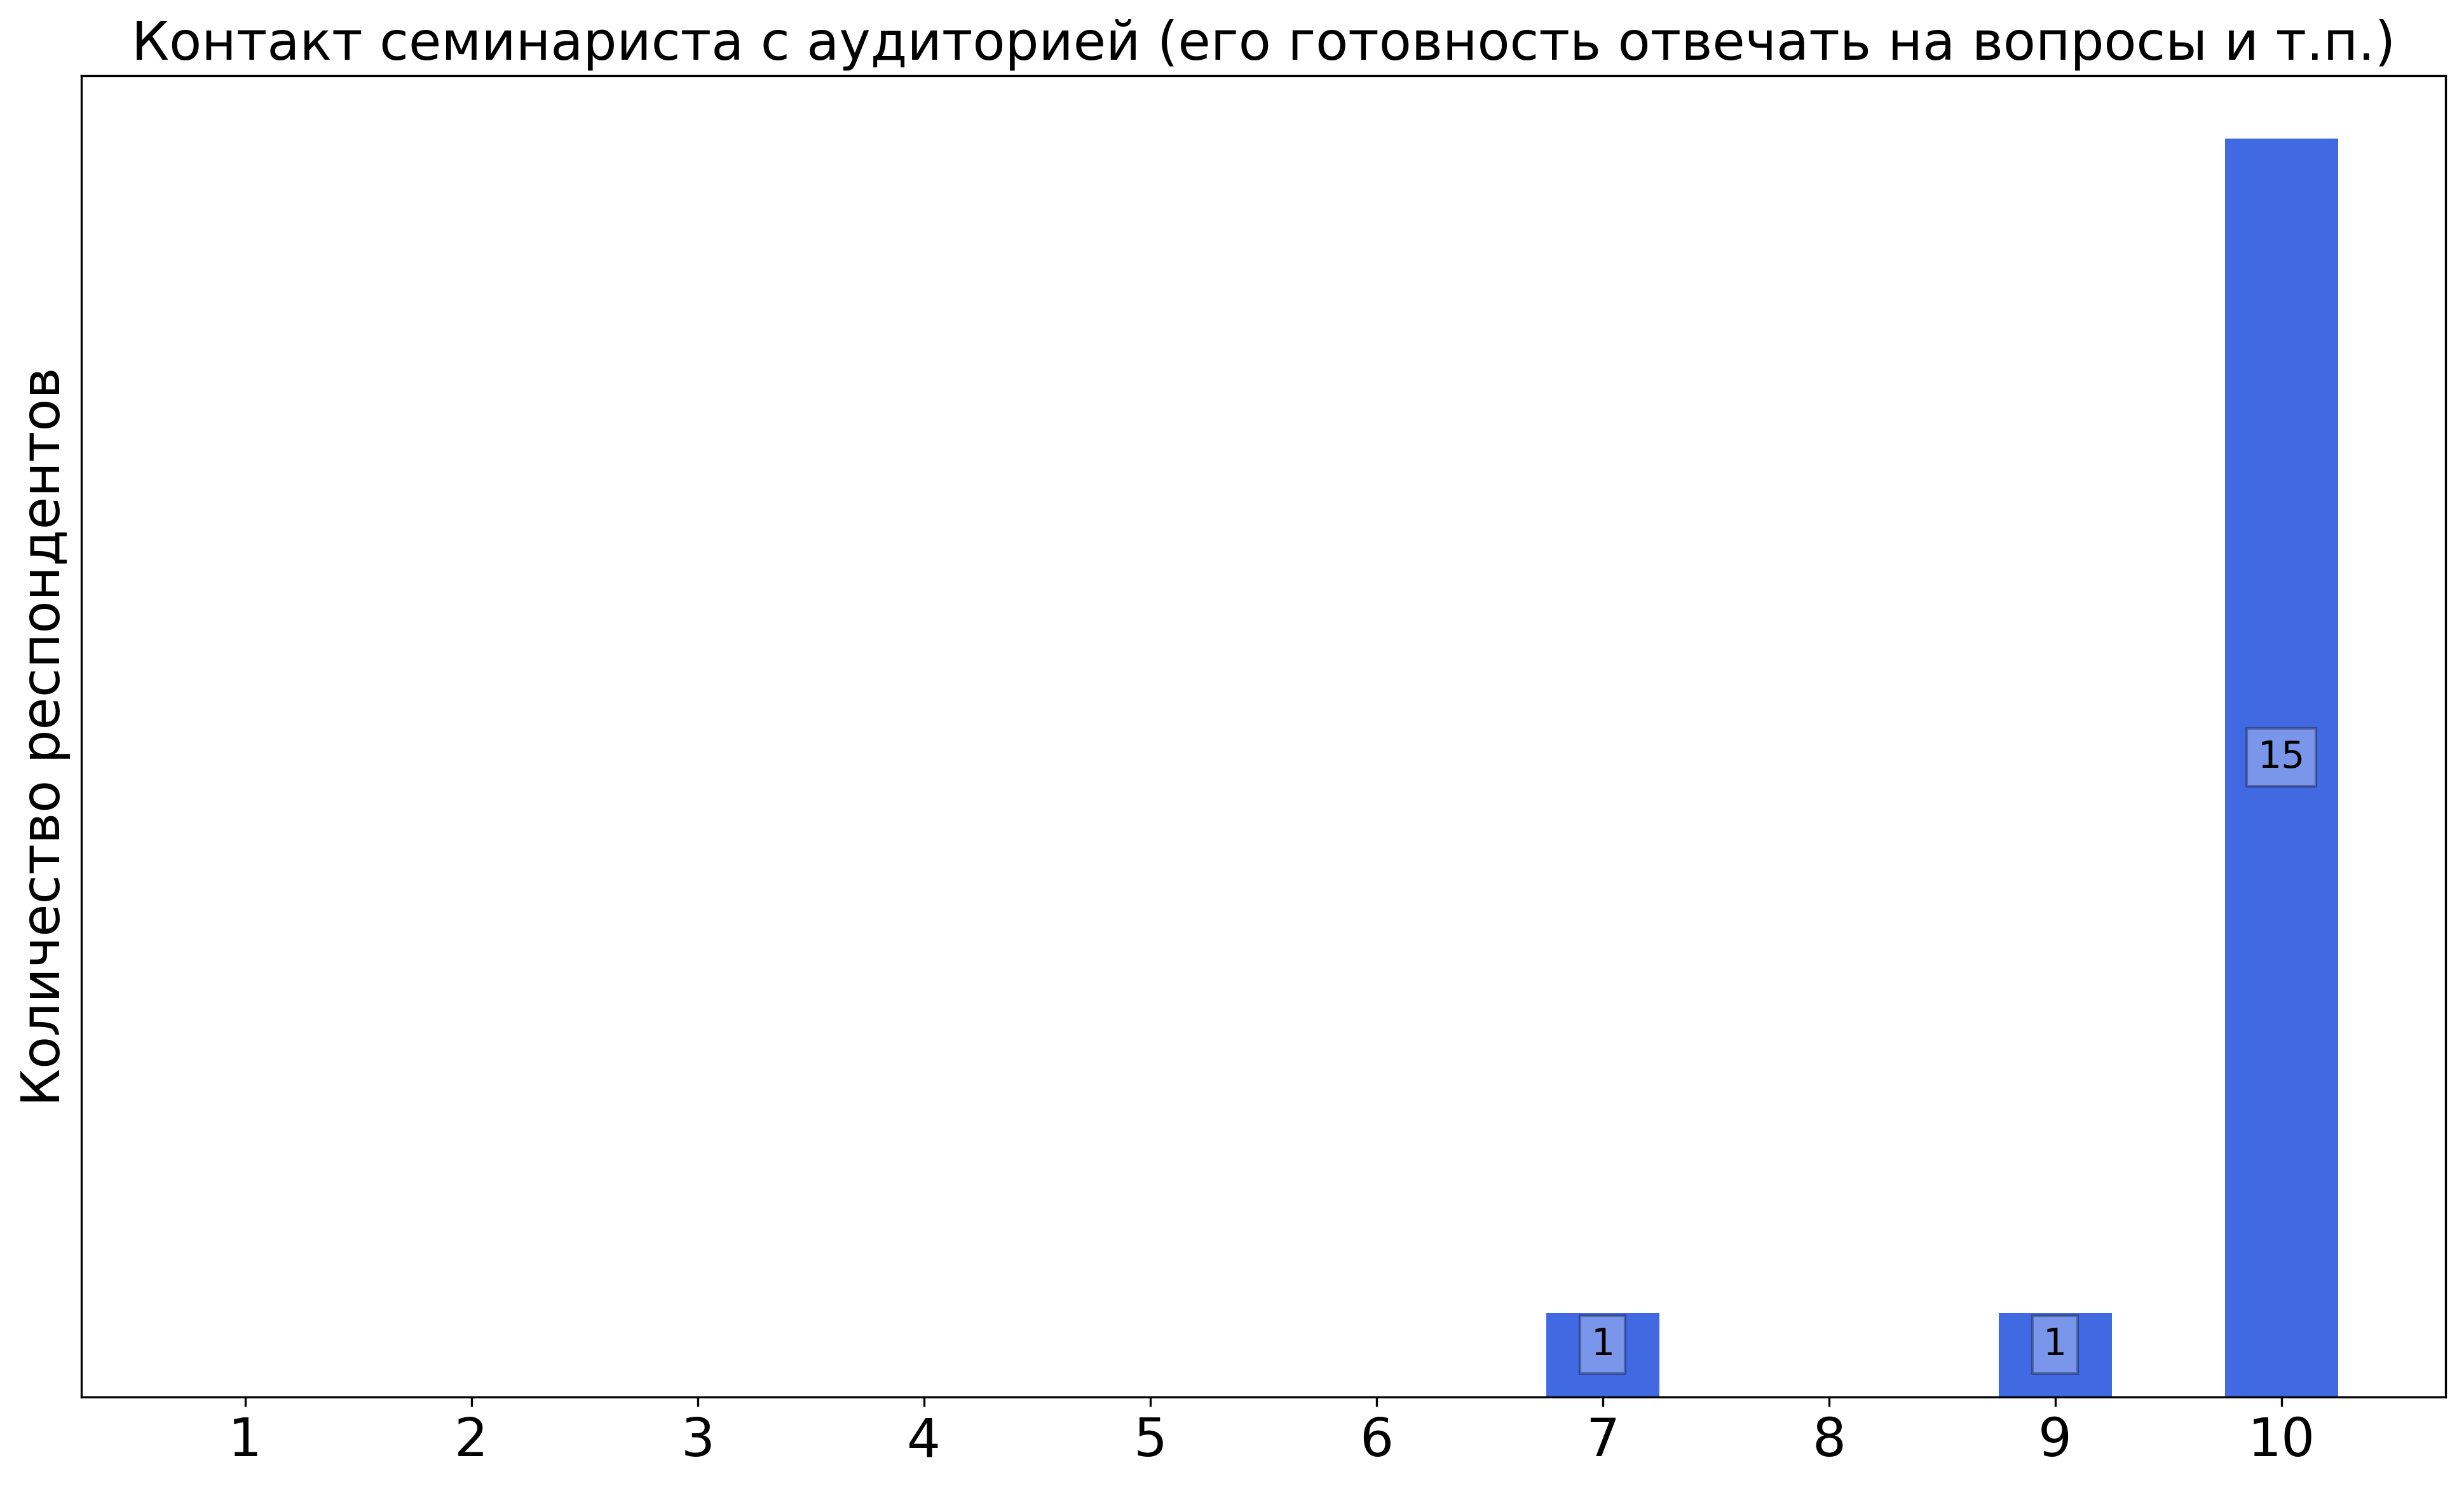
\includegraphics[width=\textwidth]{images/1 course/Математический анализ/seminarists-marks-Загрядский О.А.-0.png}
			\end{subfigure}
			\begin{subfigure}[b]{0.45\textwidth}
				\centering
				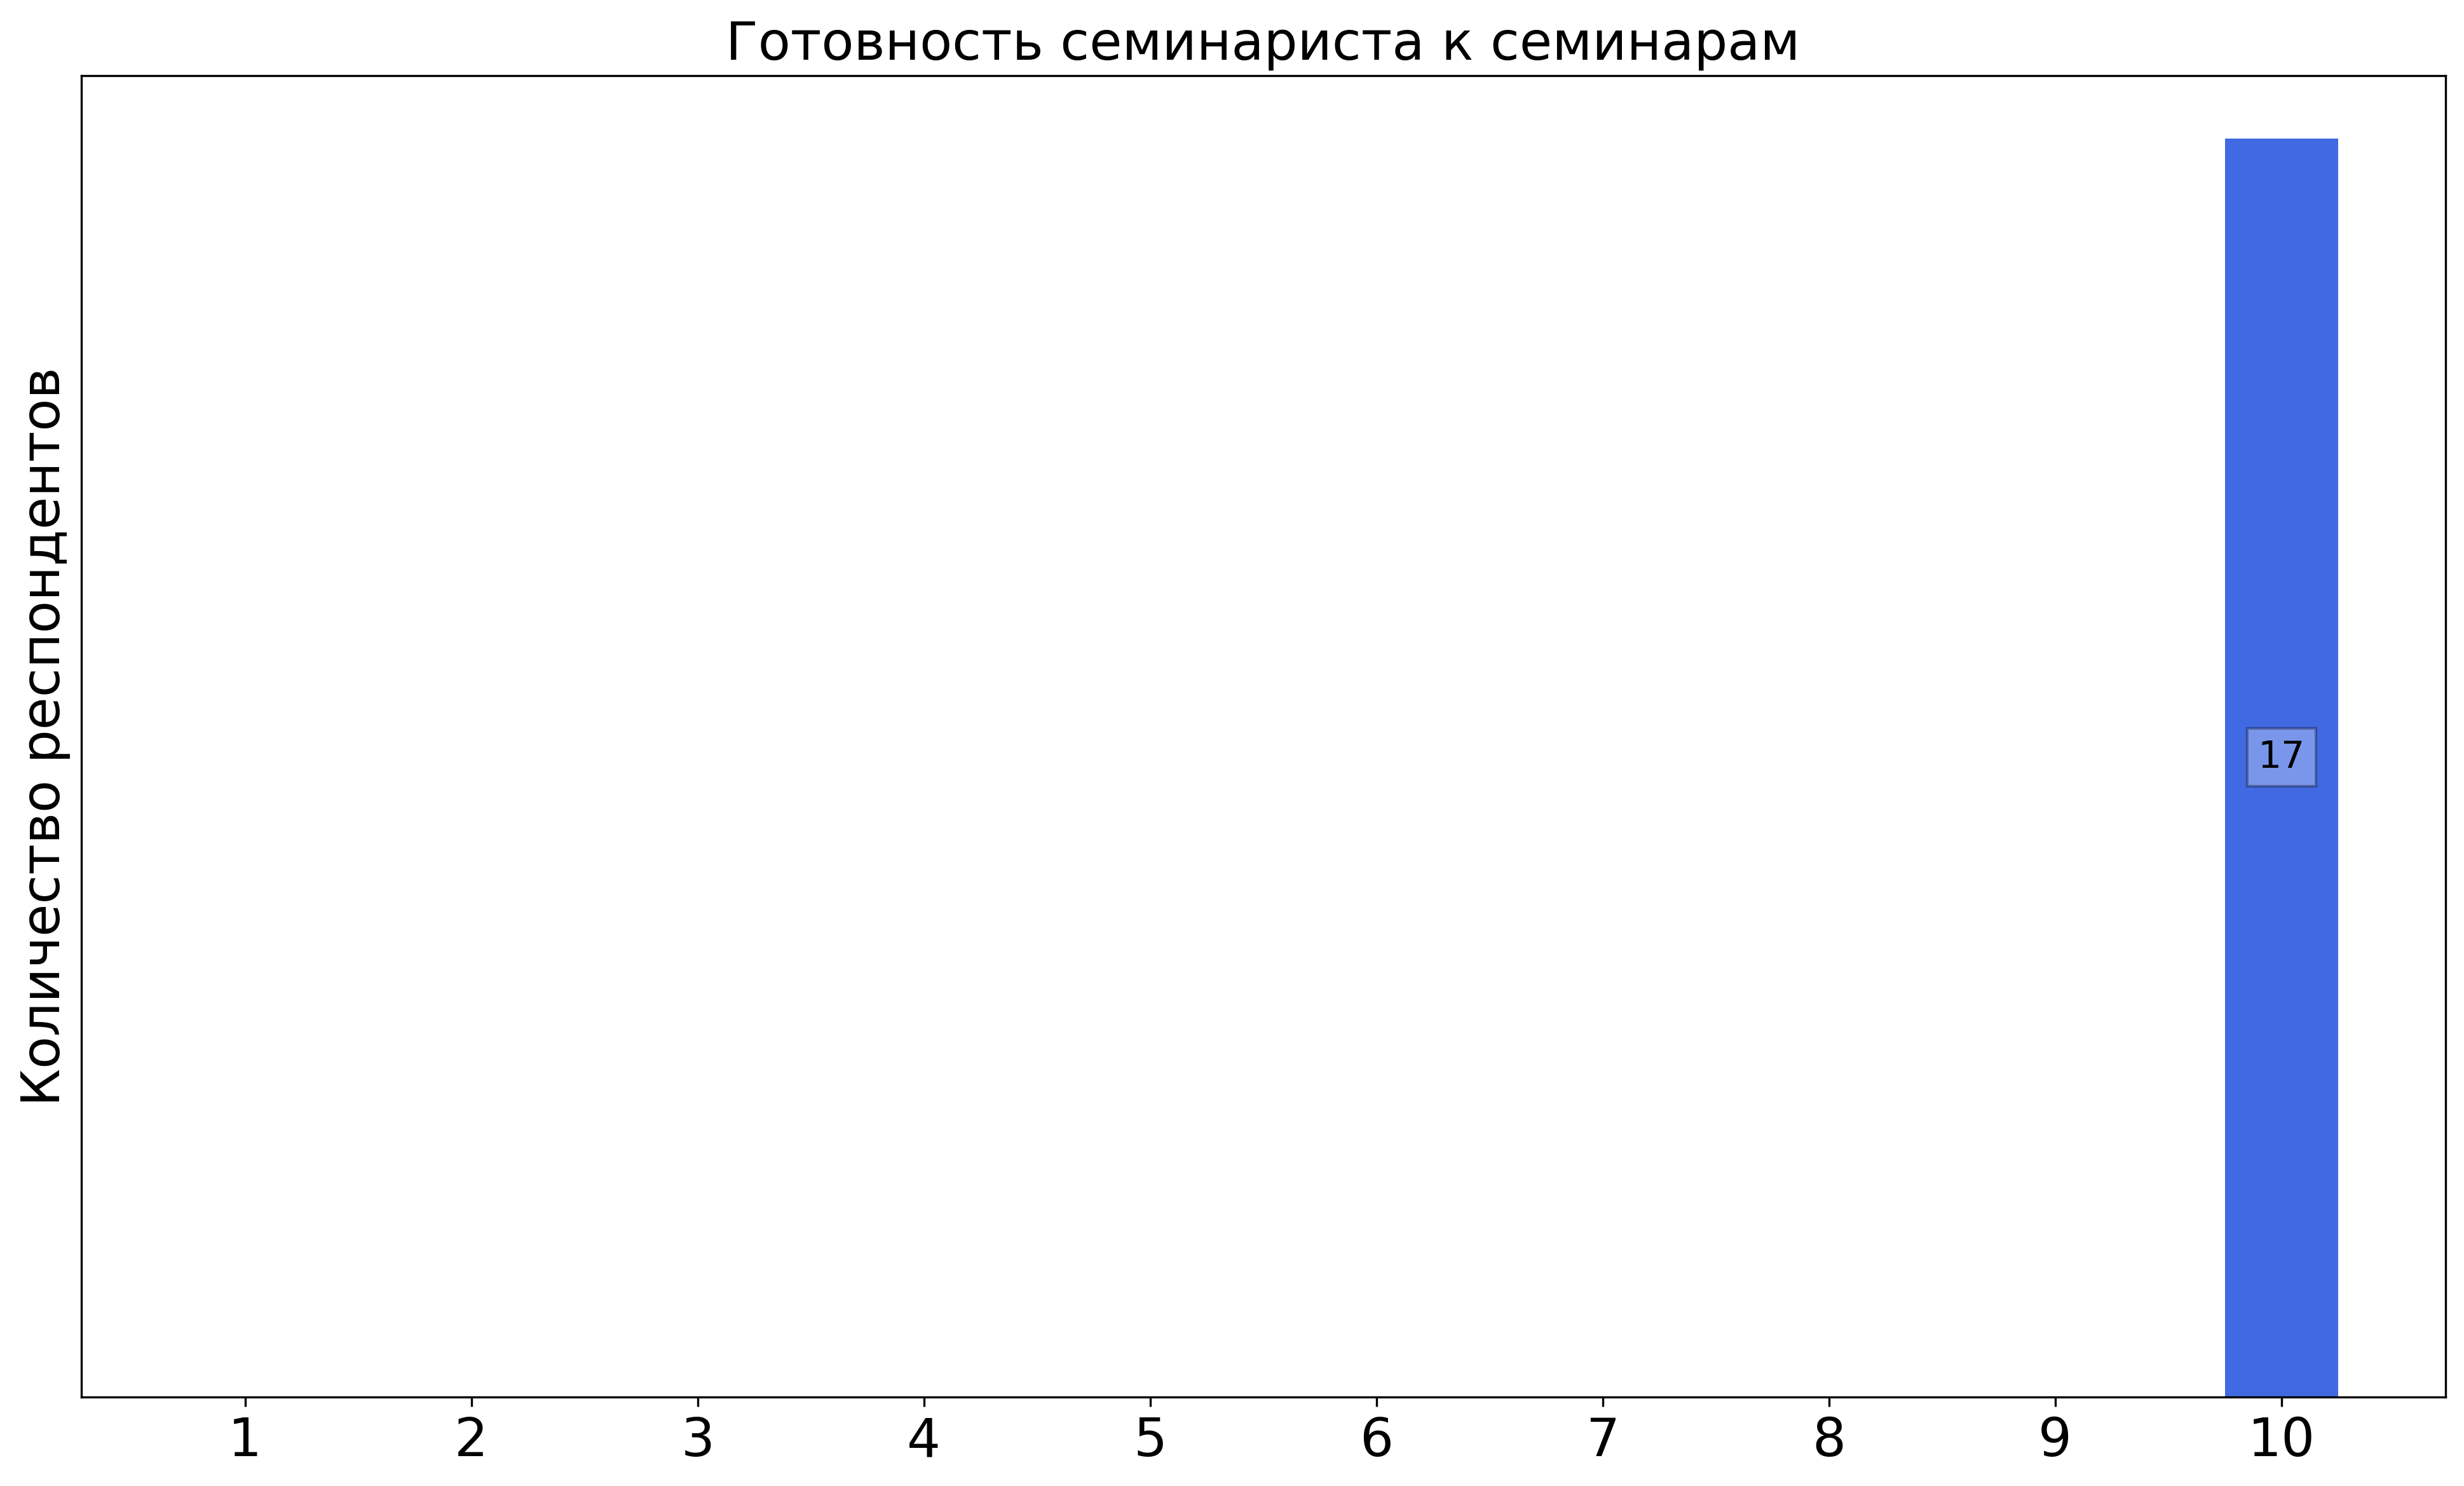
\includegraphics[width=\textwidth]{images/1 course/Математический анализ/seminarists-marks-Загрядский О.А.-1.png}
			\end{subfigure}
			\begin{subfigure}[b]{0.45\textwidth}
				\centering
				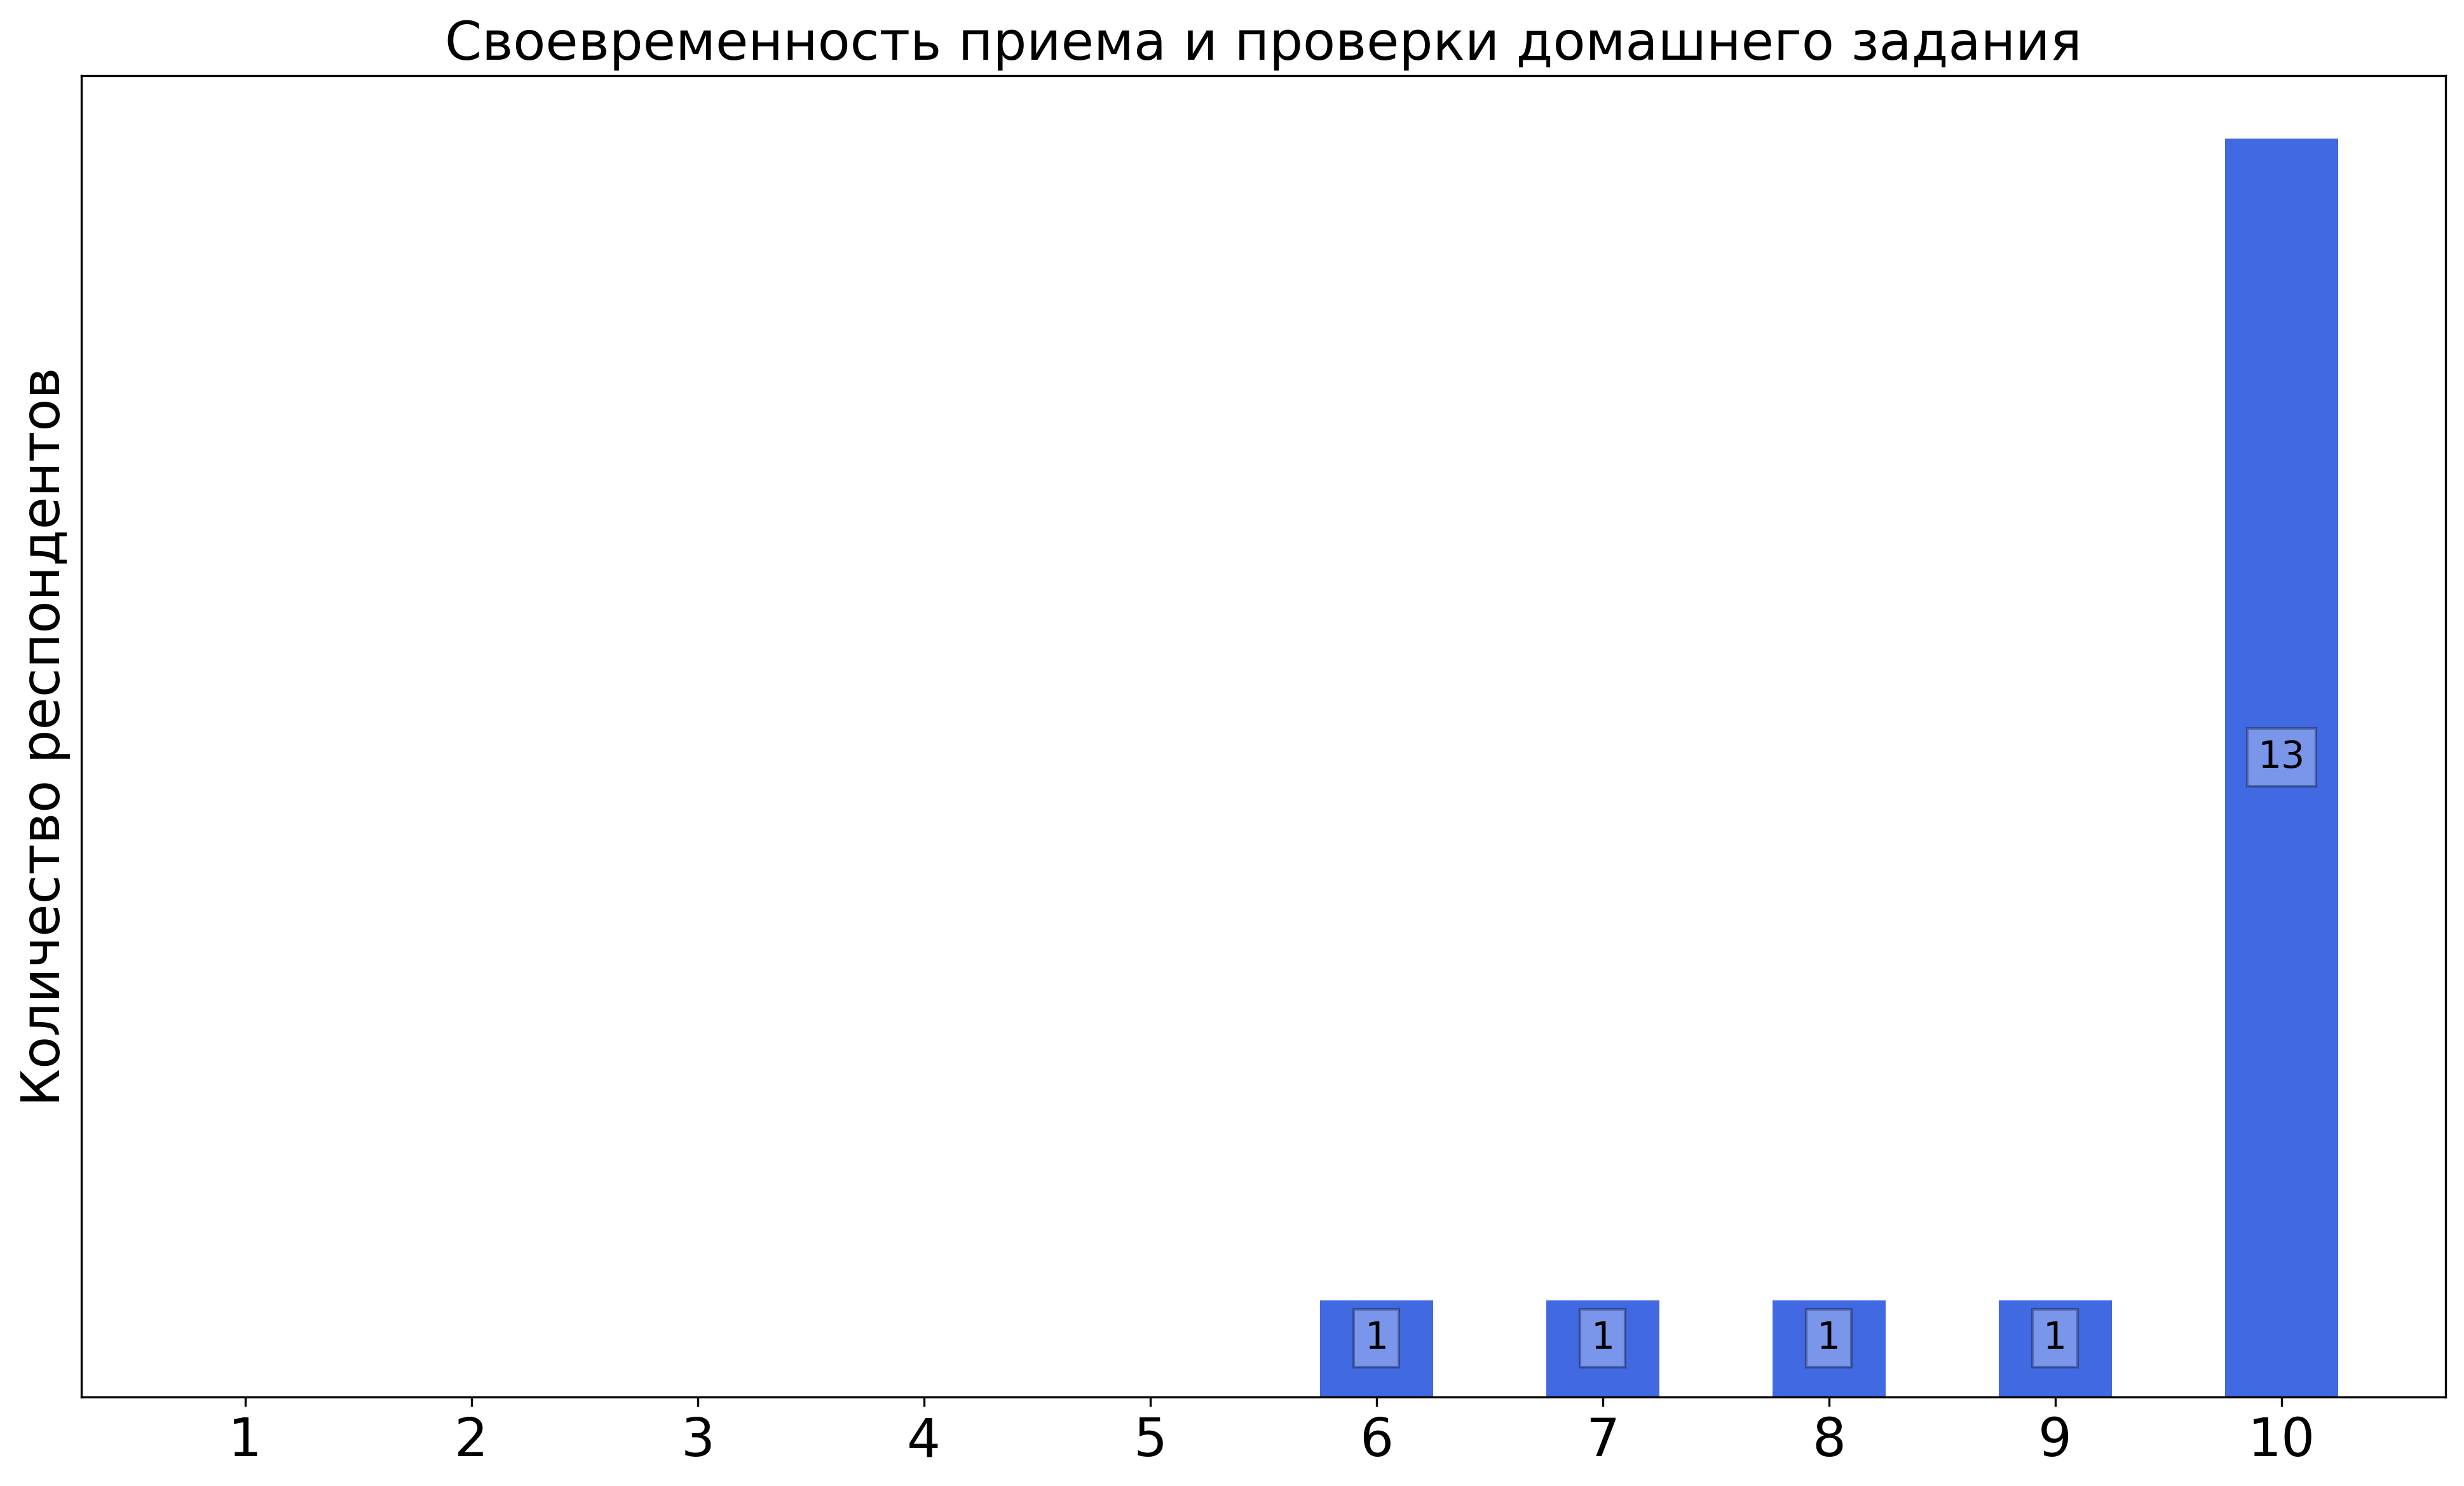
\includegraphics[width=\textwidth]{images/1 course/Математический анализ/seminarists-marks-Загрядский О.А.-2.png}
			\end{subfigure}
			\begin{subfigure}[b]{0.45\textwidth}
				\centering
				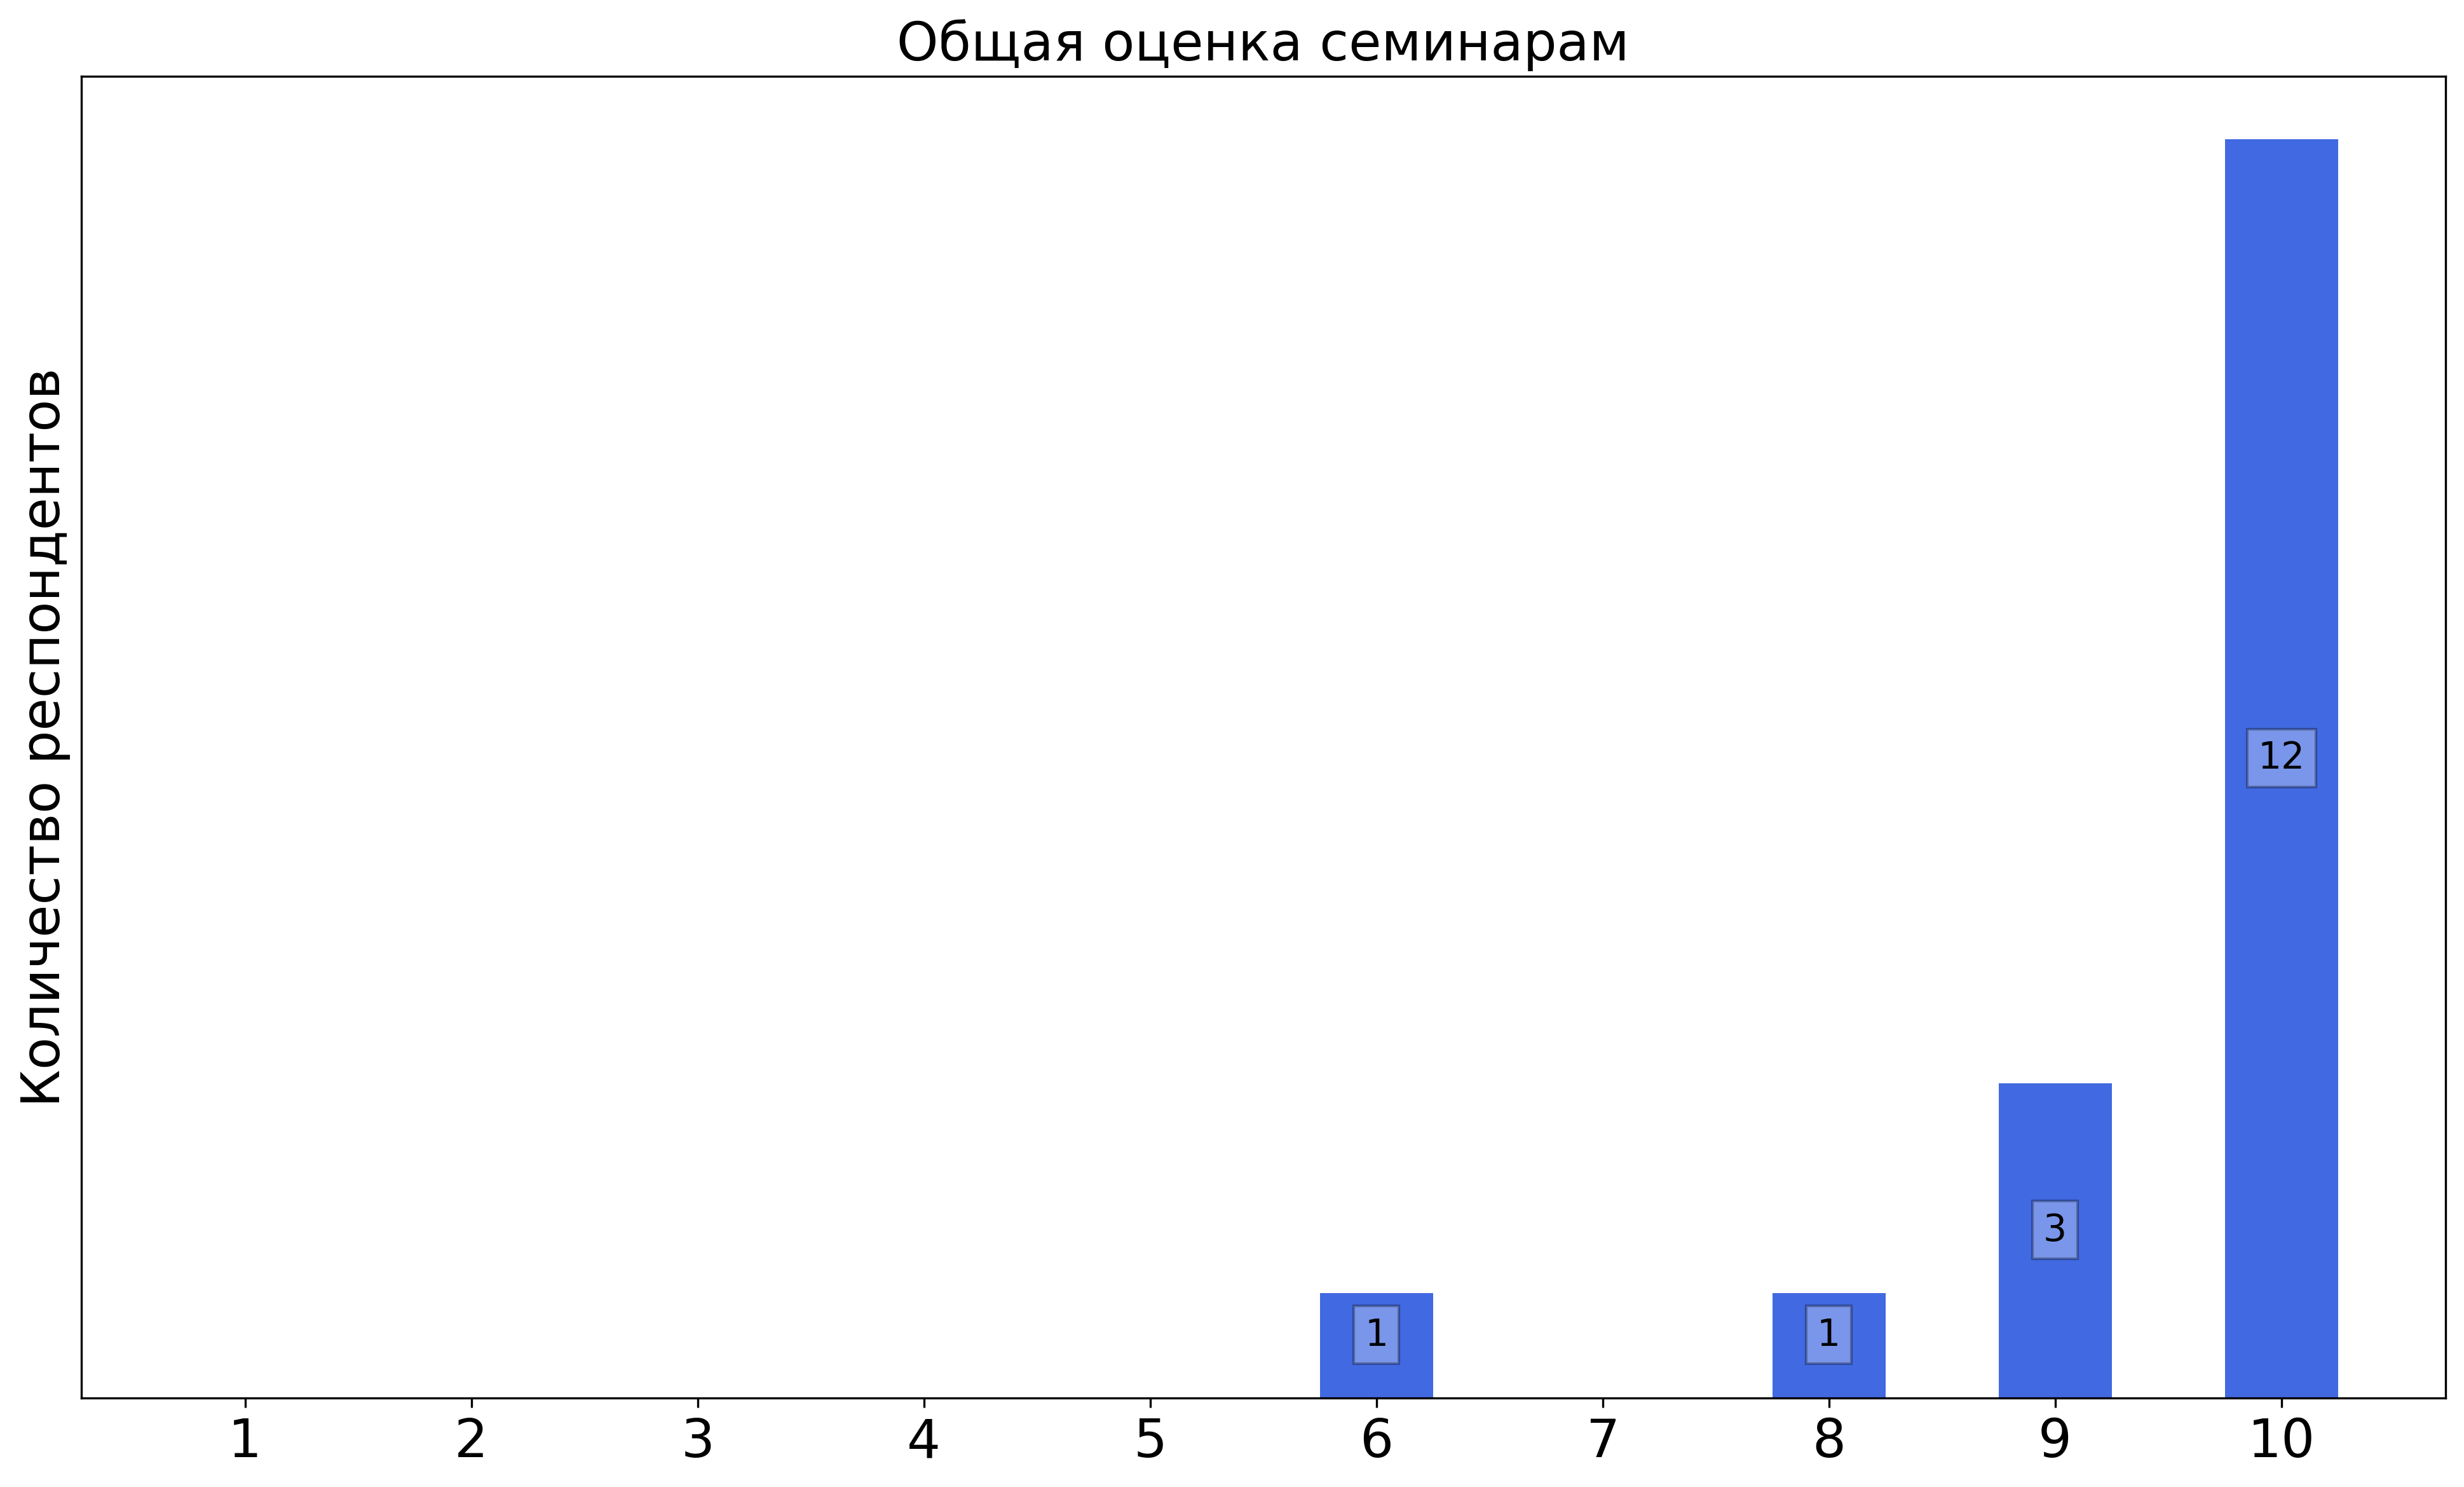
\includegraphics[width=\textwidth]{images/1 course/Математический анализ/seminarists-marks-Загрядский О.А.-3.png}
			\end{subfigure}	
			\caption{Оценки респондентов о качестве преподавания семинаров}
		\end{figure}

		\textbf{Комментарии студентов о семинаристе\protect\footnote{сохранены оригинальные орфография и пунктуация}}
			\begin{commentbox} 
				Человек в плане оценивания жесткий, но благодаря этому к сессии по матану можно было не готовиться 
			\end{commentbox} 
		
			\begin{commentbox} 
				Отличный семинарист, лучше наверное и быть не может. 
			\end{commentbox} 
		
			\begin{commentbox} 
				Прекрасный семинарист 
			\end{commentbox} 
		
			\begin{commentbox} 
				лучший семинарист из возможных 
			\end{commentbox} 
		
			\begin{commentbox} 
				Загромамонт очень достойный семинарист.  
			\end{commentbox} 
		
			\begin{commentbox} 
				Просто лучший, все, что нужно, расшарит, допсем при необходимости проведет, в тг на все вопросы ответит и пойдет с коллегами пить чай. 12 мумитроллей из 10 
			\end{commentbox} 
		
			\begin{commentbox} 
				Шарящий семинарис, который может изложить и объяснить материал на любом уровне. Для особо интересующихся проводил кружки.  
			\end{commentbox} 
		
			\begin{commentbox} 
				Старается прислушиваться к мнению студентов, подстраивается под их уровень. С большим удовольствием готов изложить дополнительный материал. (Но поначалу его изложение кажется слишком быстрым и от этого снижается понимание) 
			\end{commentbox} 
		
			\begin{commentbox} 
				Лучший! 
			\end{commentbox} 
		
			\begin{commentbox} 
				Загрядский действительно шарит в предмете, проводит допы, постоянно просит, чтобы ему задавали вопросы. 
			\end{commentbox}
				

	\subsubsection{Отзыв студентов о семинарах. Семинарист: Знаменская Л.Н.}		
		\begin{figure}[H]
			\centering
			\begin{subfigure}[b]{0.45\textwidth}
				\centering
				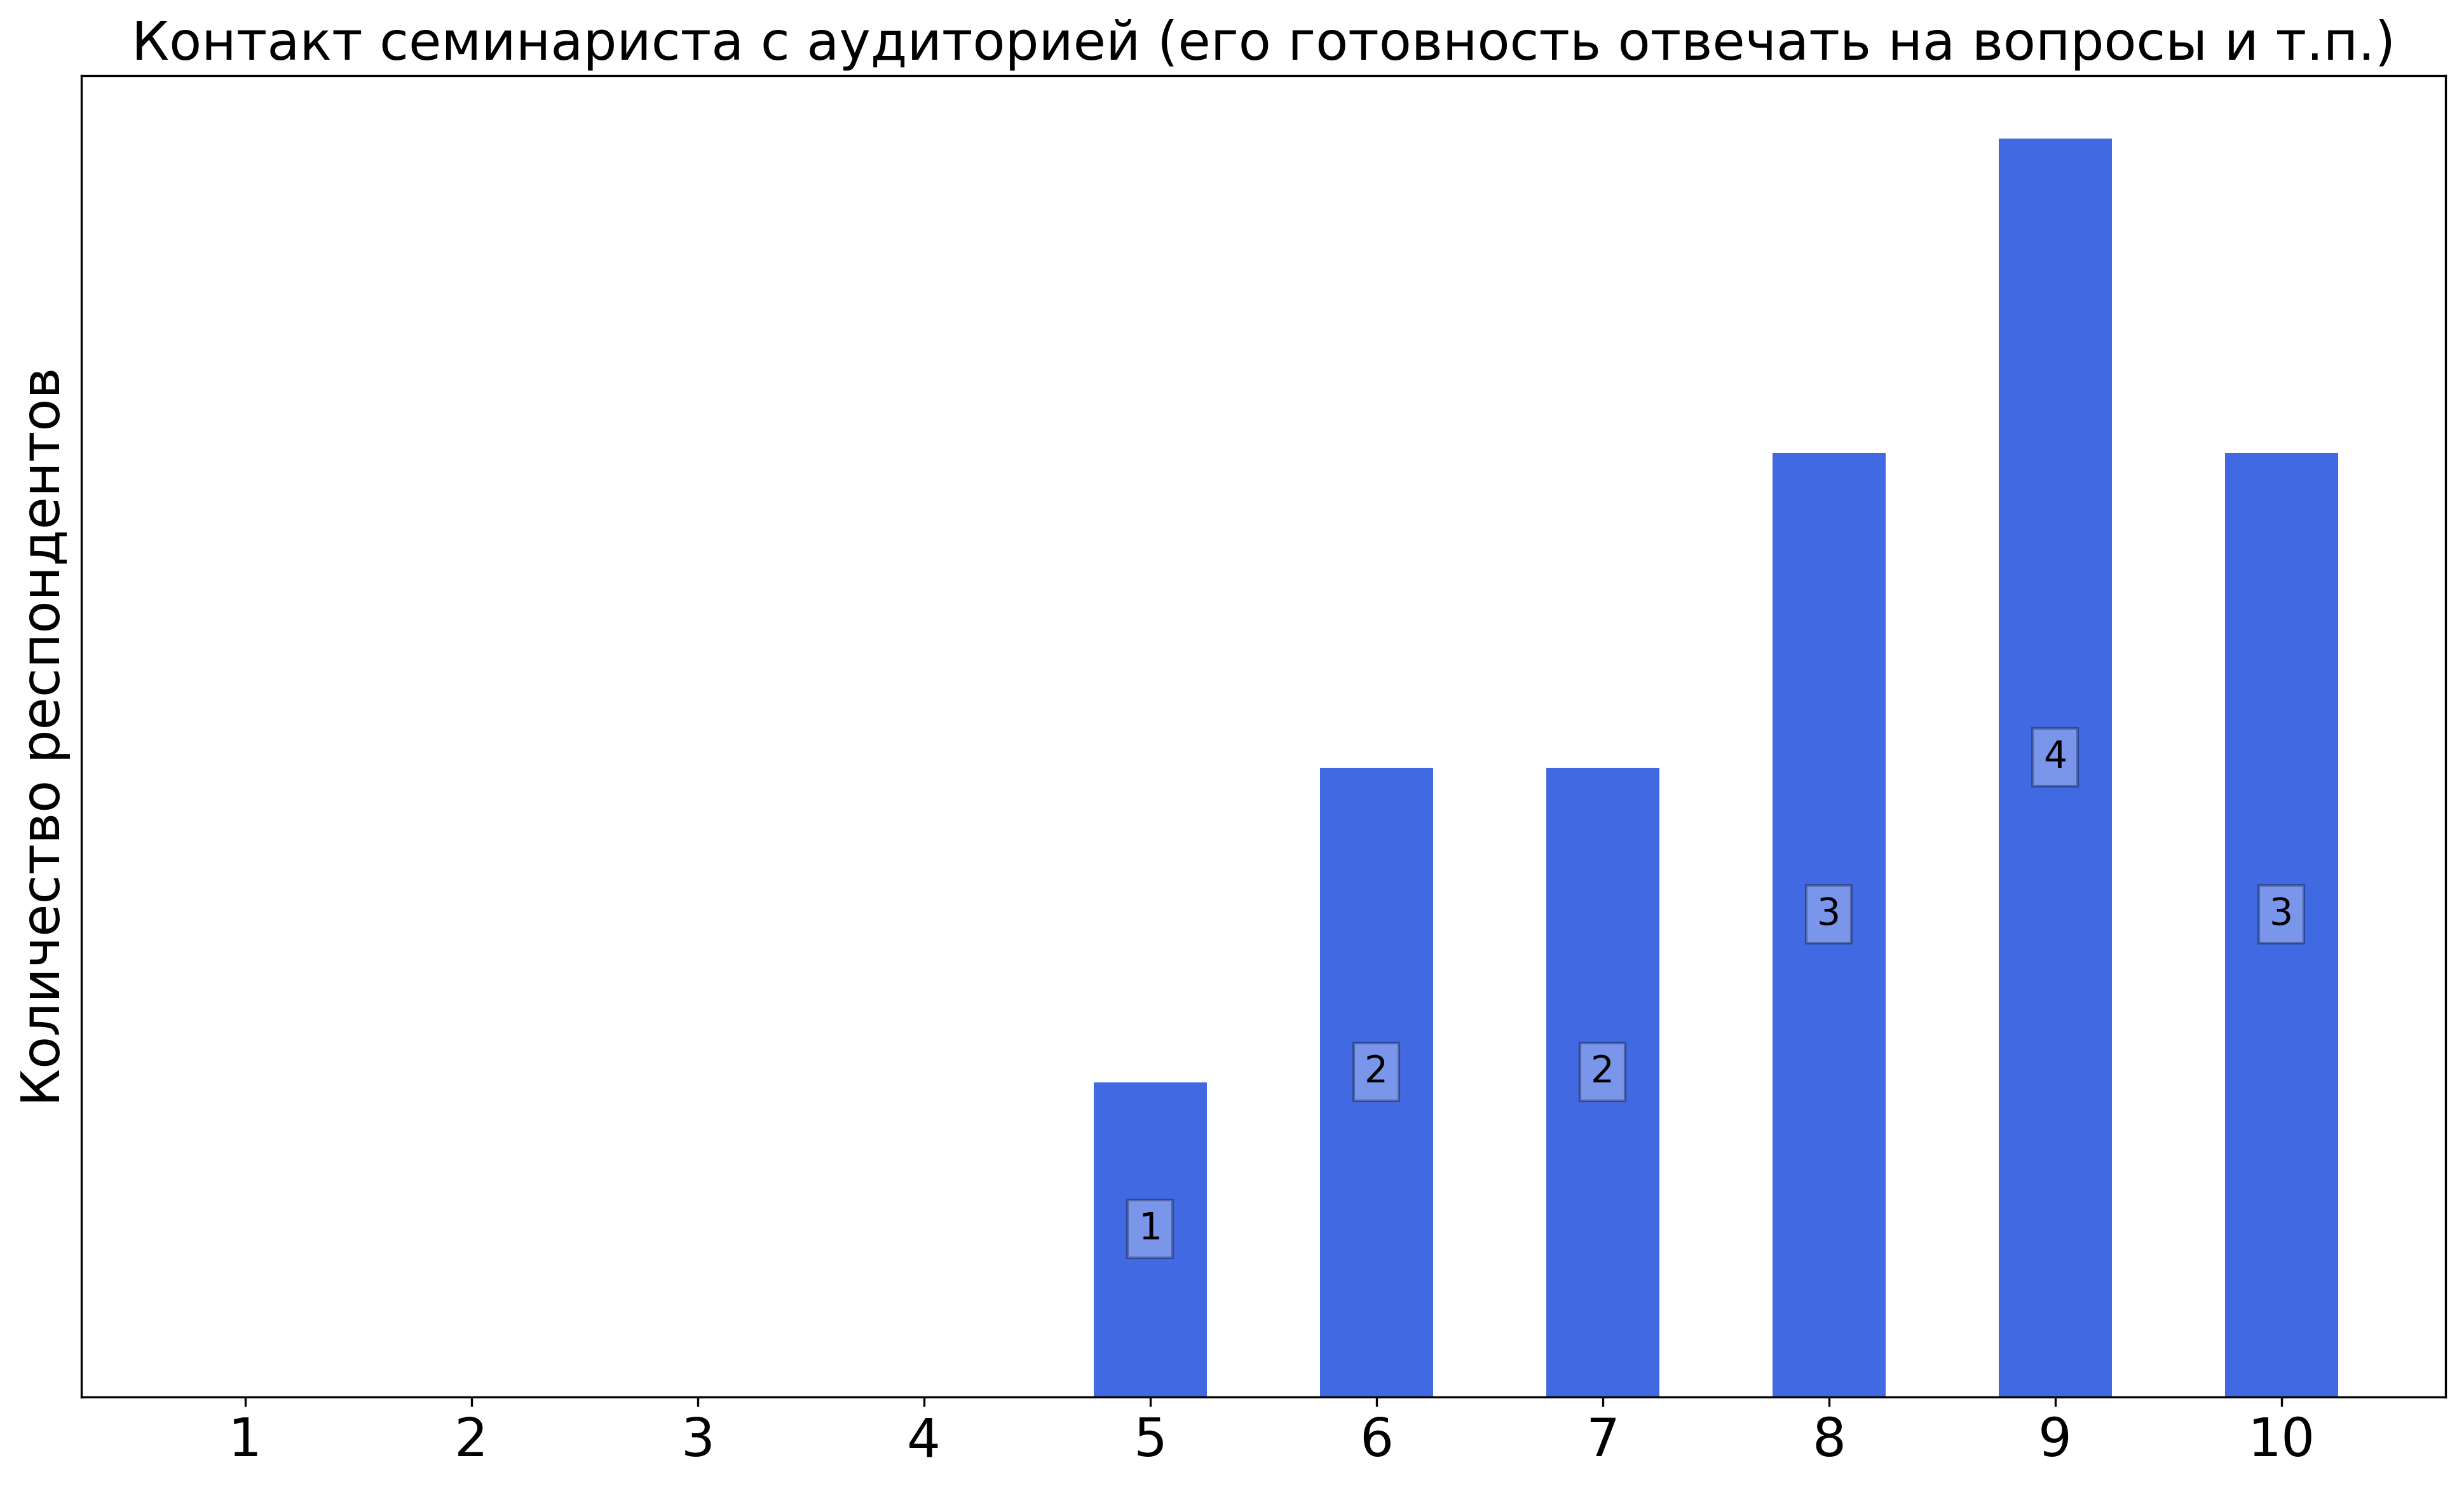
\includegraphics[width=\textwidth]{images/1 course/Математический анализ/seminarists-marks-Знаменская Л.Н.-0.png}
			\end{subfigure}
			\begin{subfigure}[b]{0.45\textwidth}
				\centering
				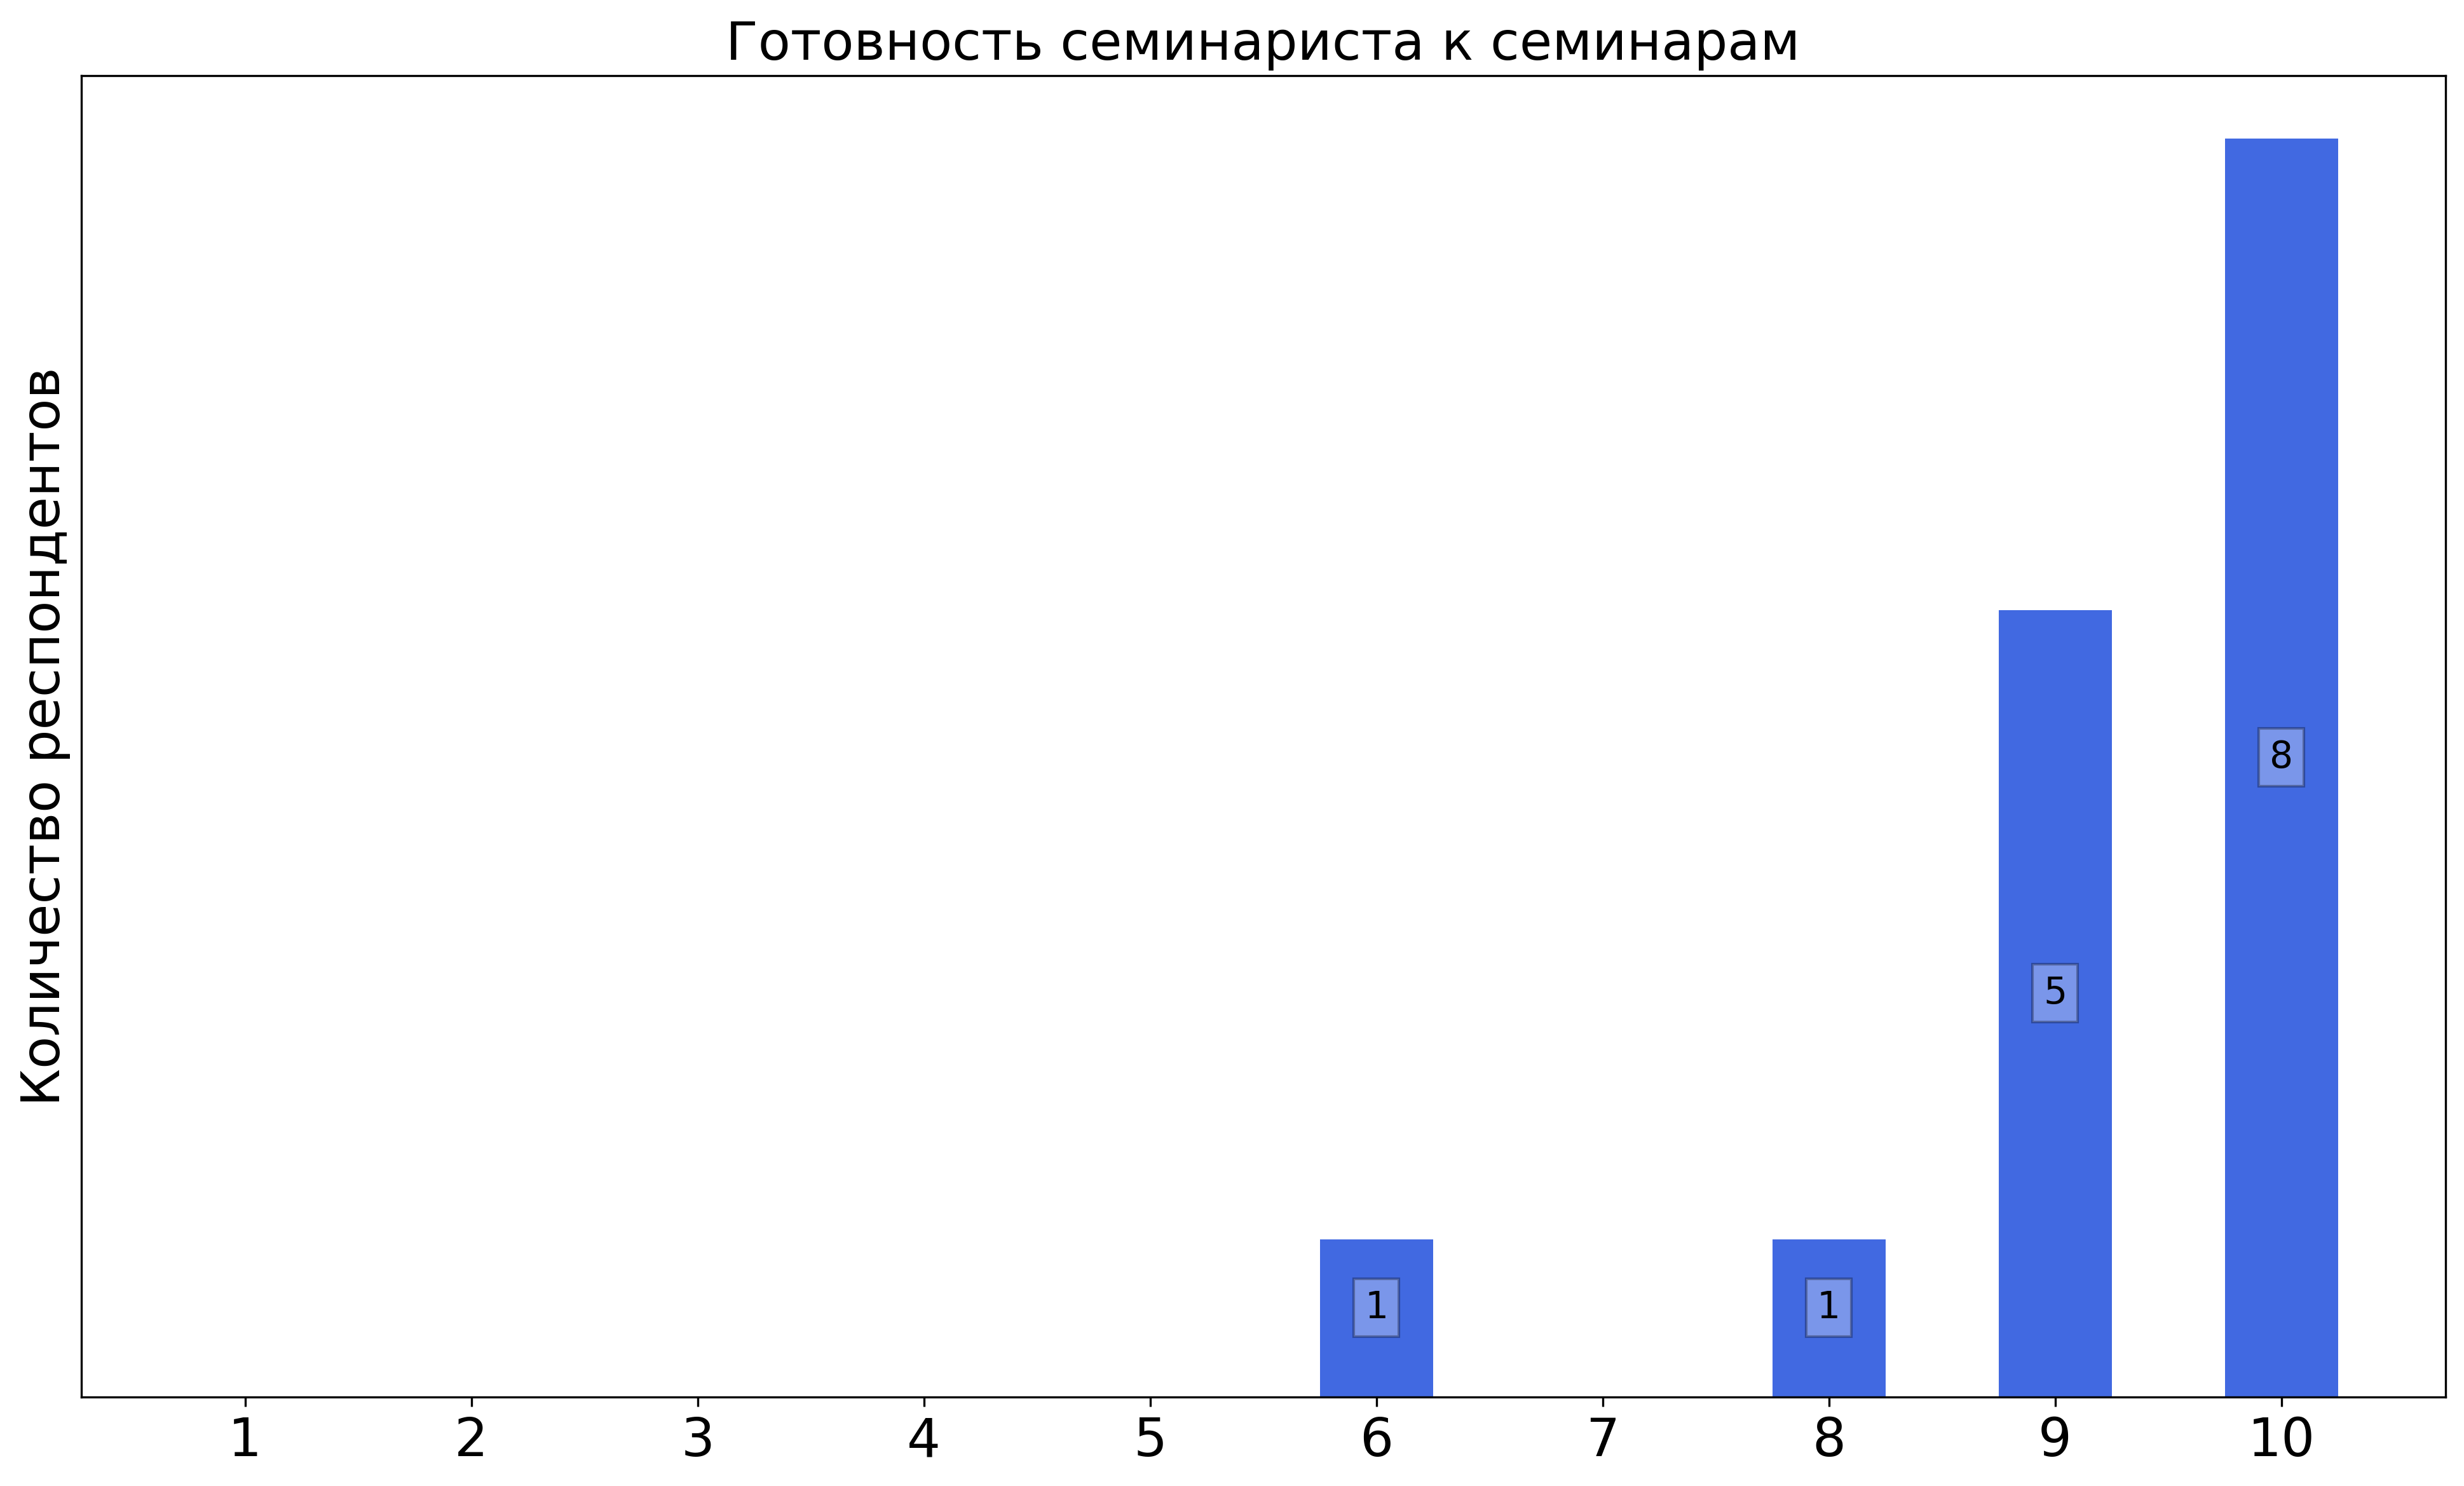
\includegraphics[width=\textwidth]{images/1 course/Математический анализ/seminarists-marks-Знаменская Л.Н.-1.png}
			\end{subfigure}
			\begin{subfigure}[b]{0.45\textwidth}
				\centering
				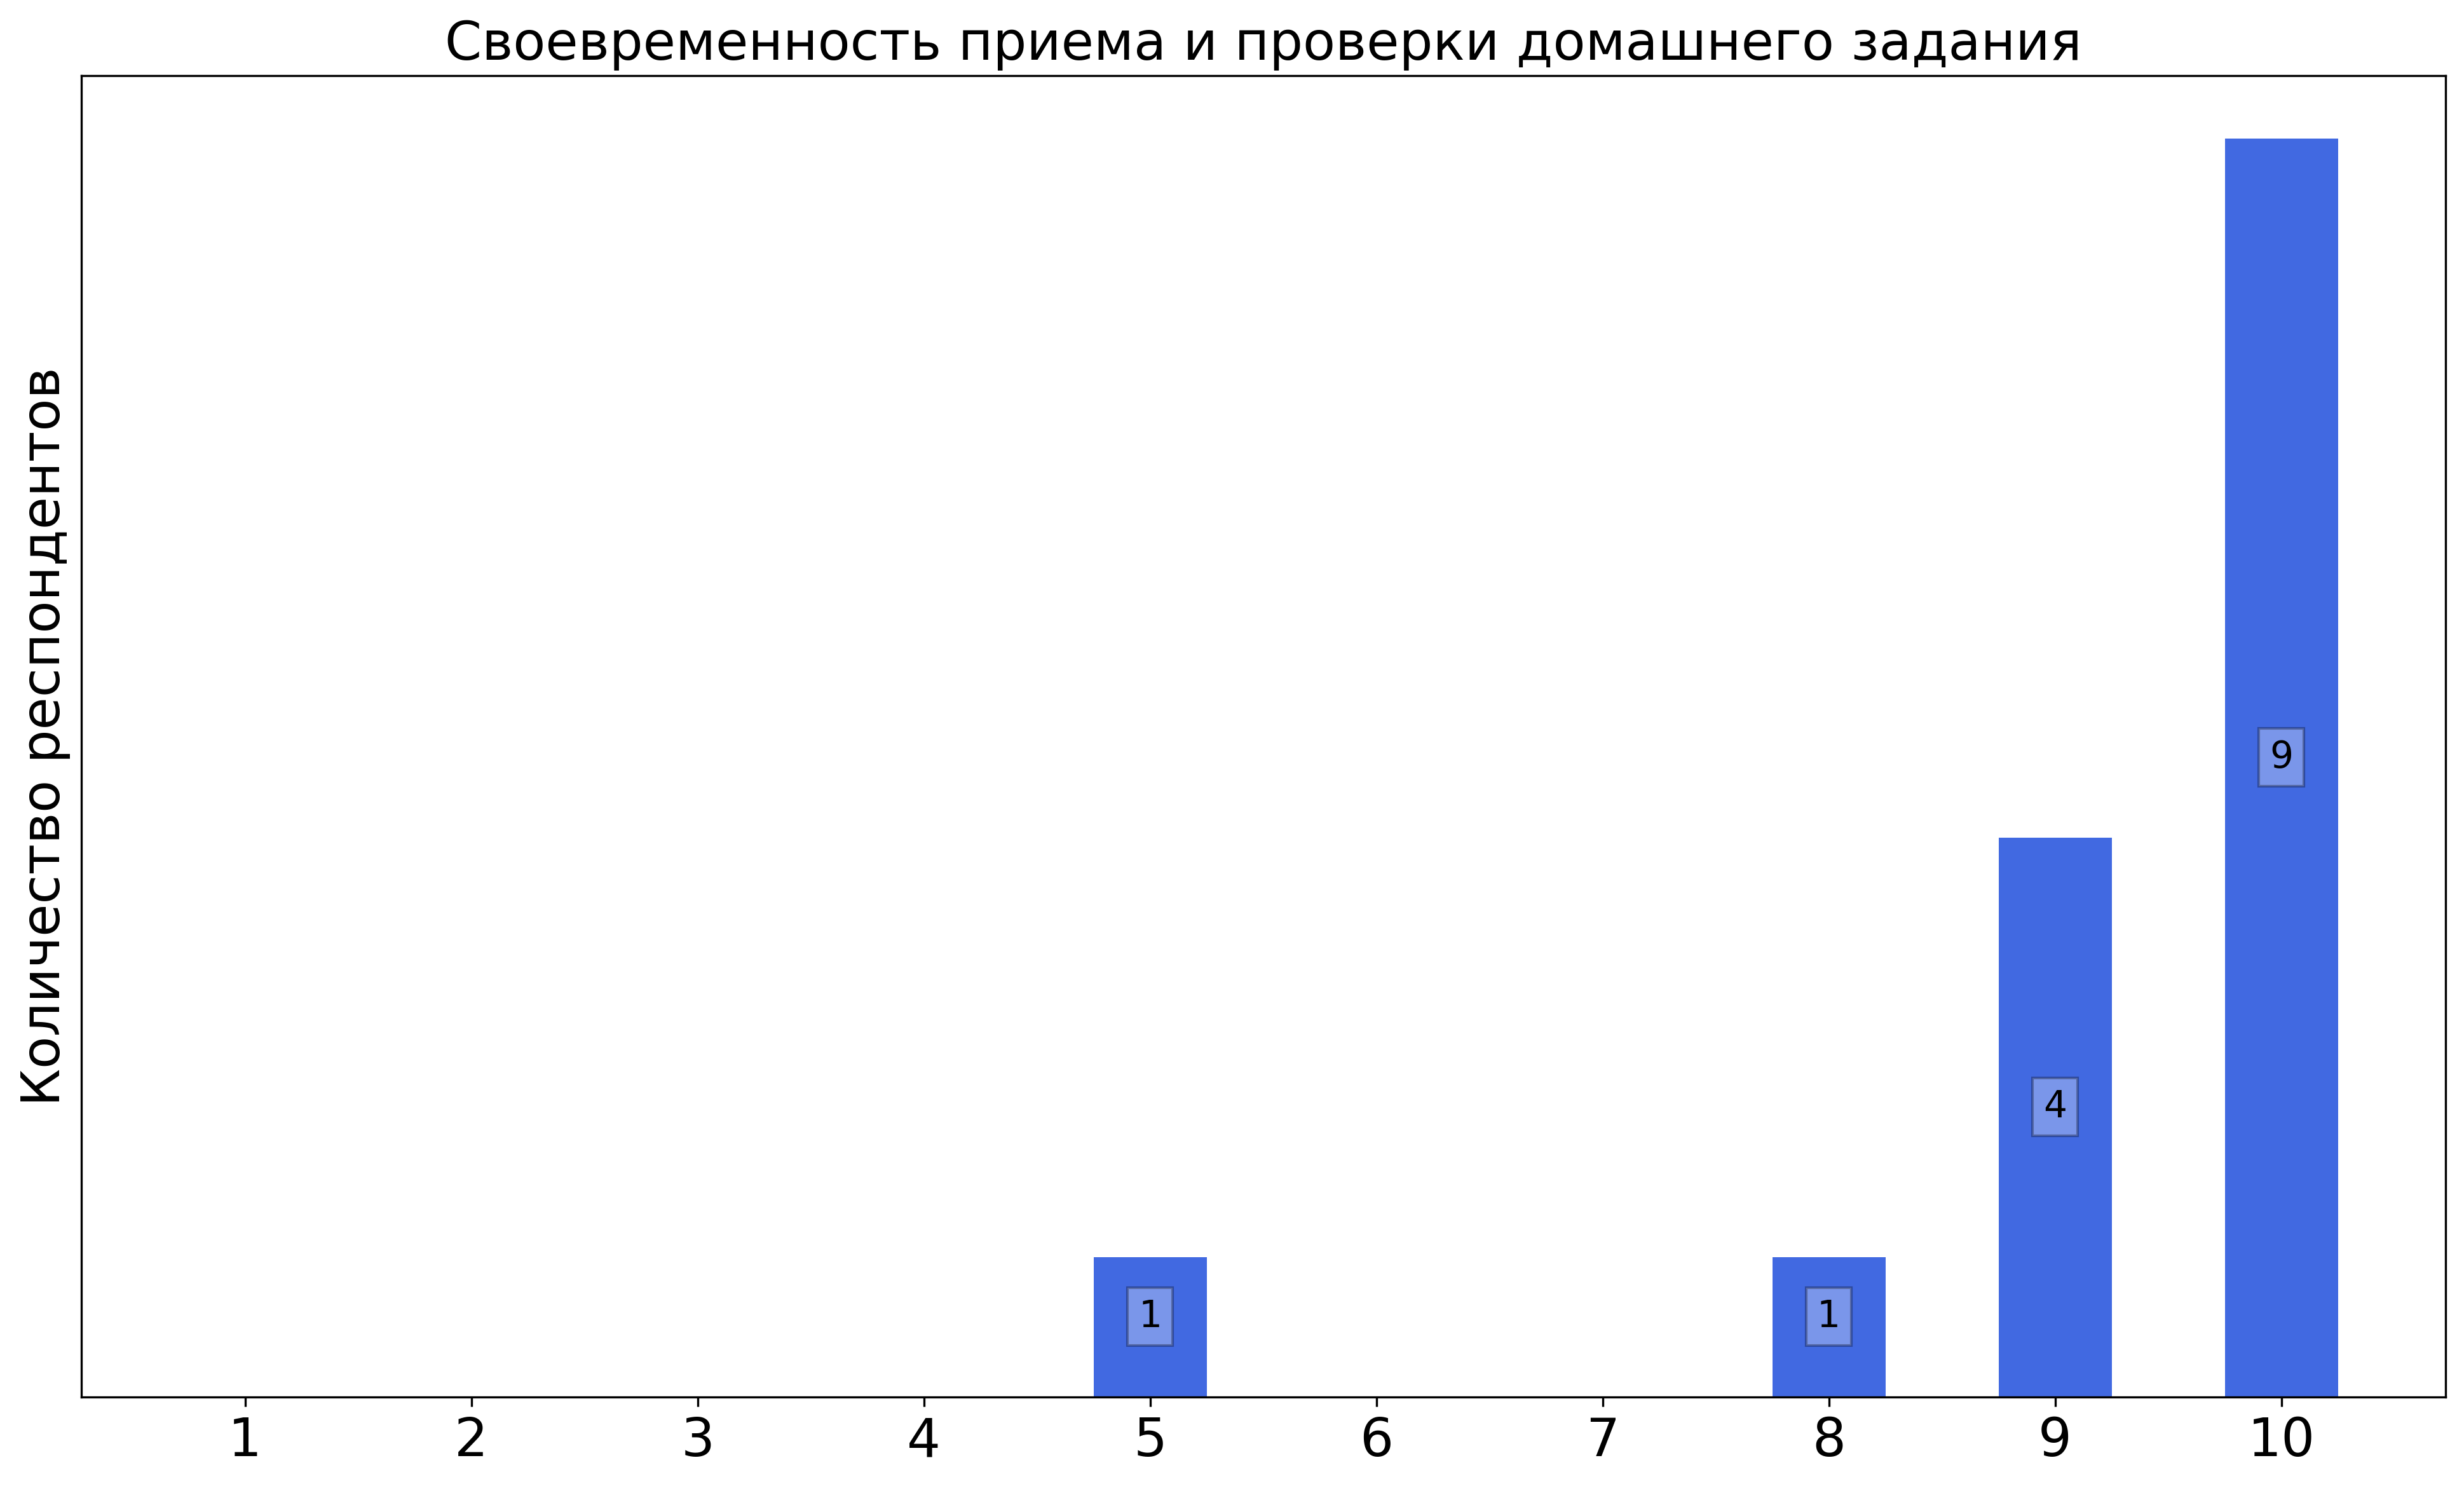
\includegraphics[width=\textwidth]{images/1 course/Математический анализ/seminarists-marks-Знаменская Л.Н.-2.png}
			\end{subfigure}
			\begin{subfigure}[b]{0.45\textwidth}
				\centering
				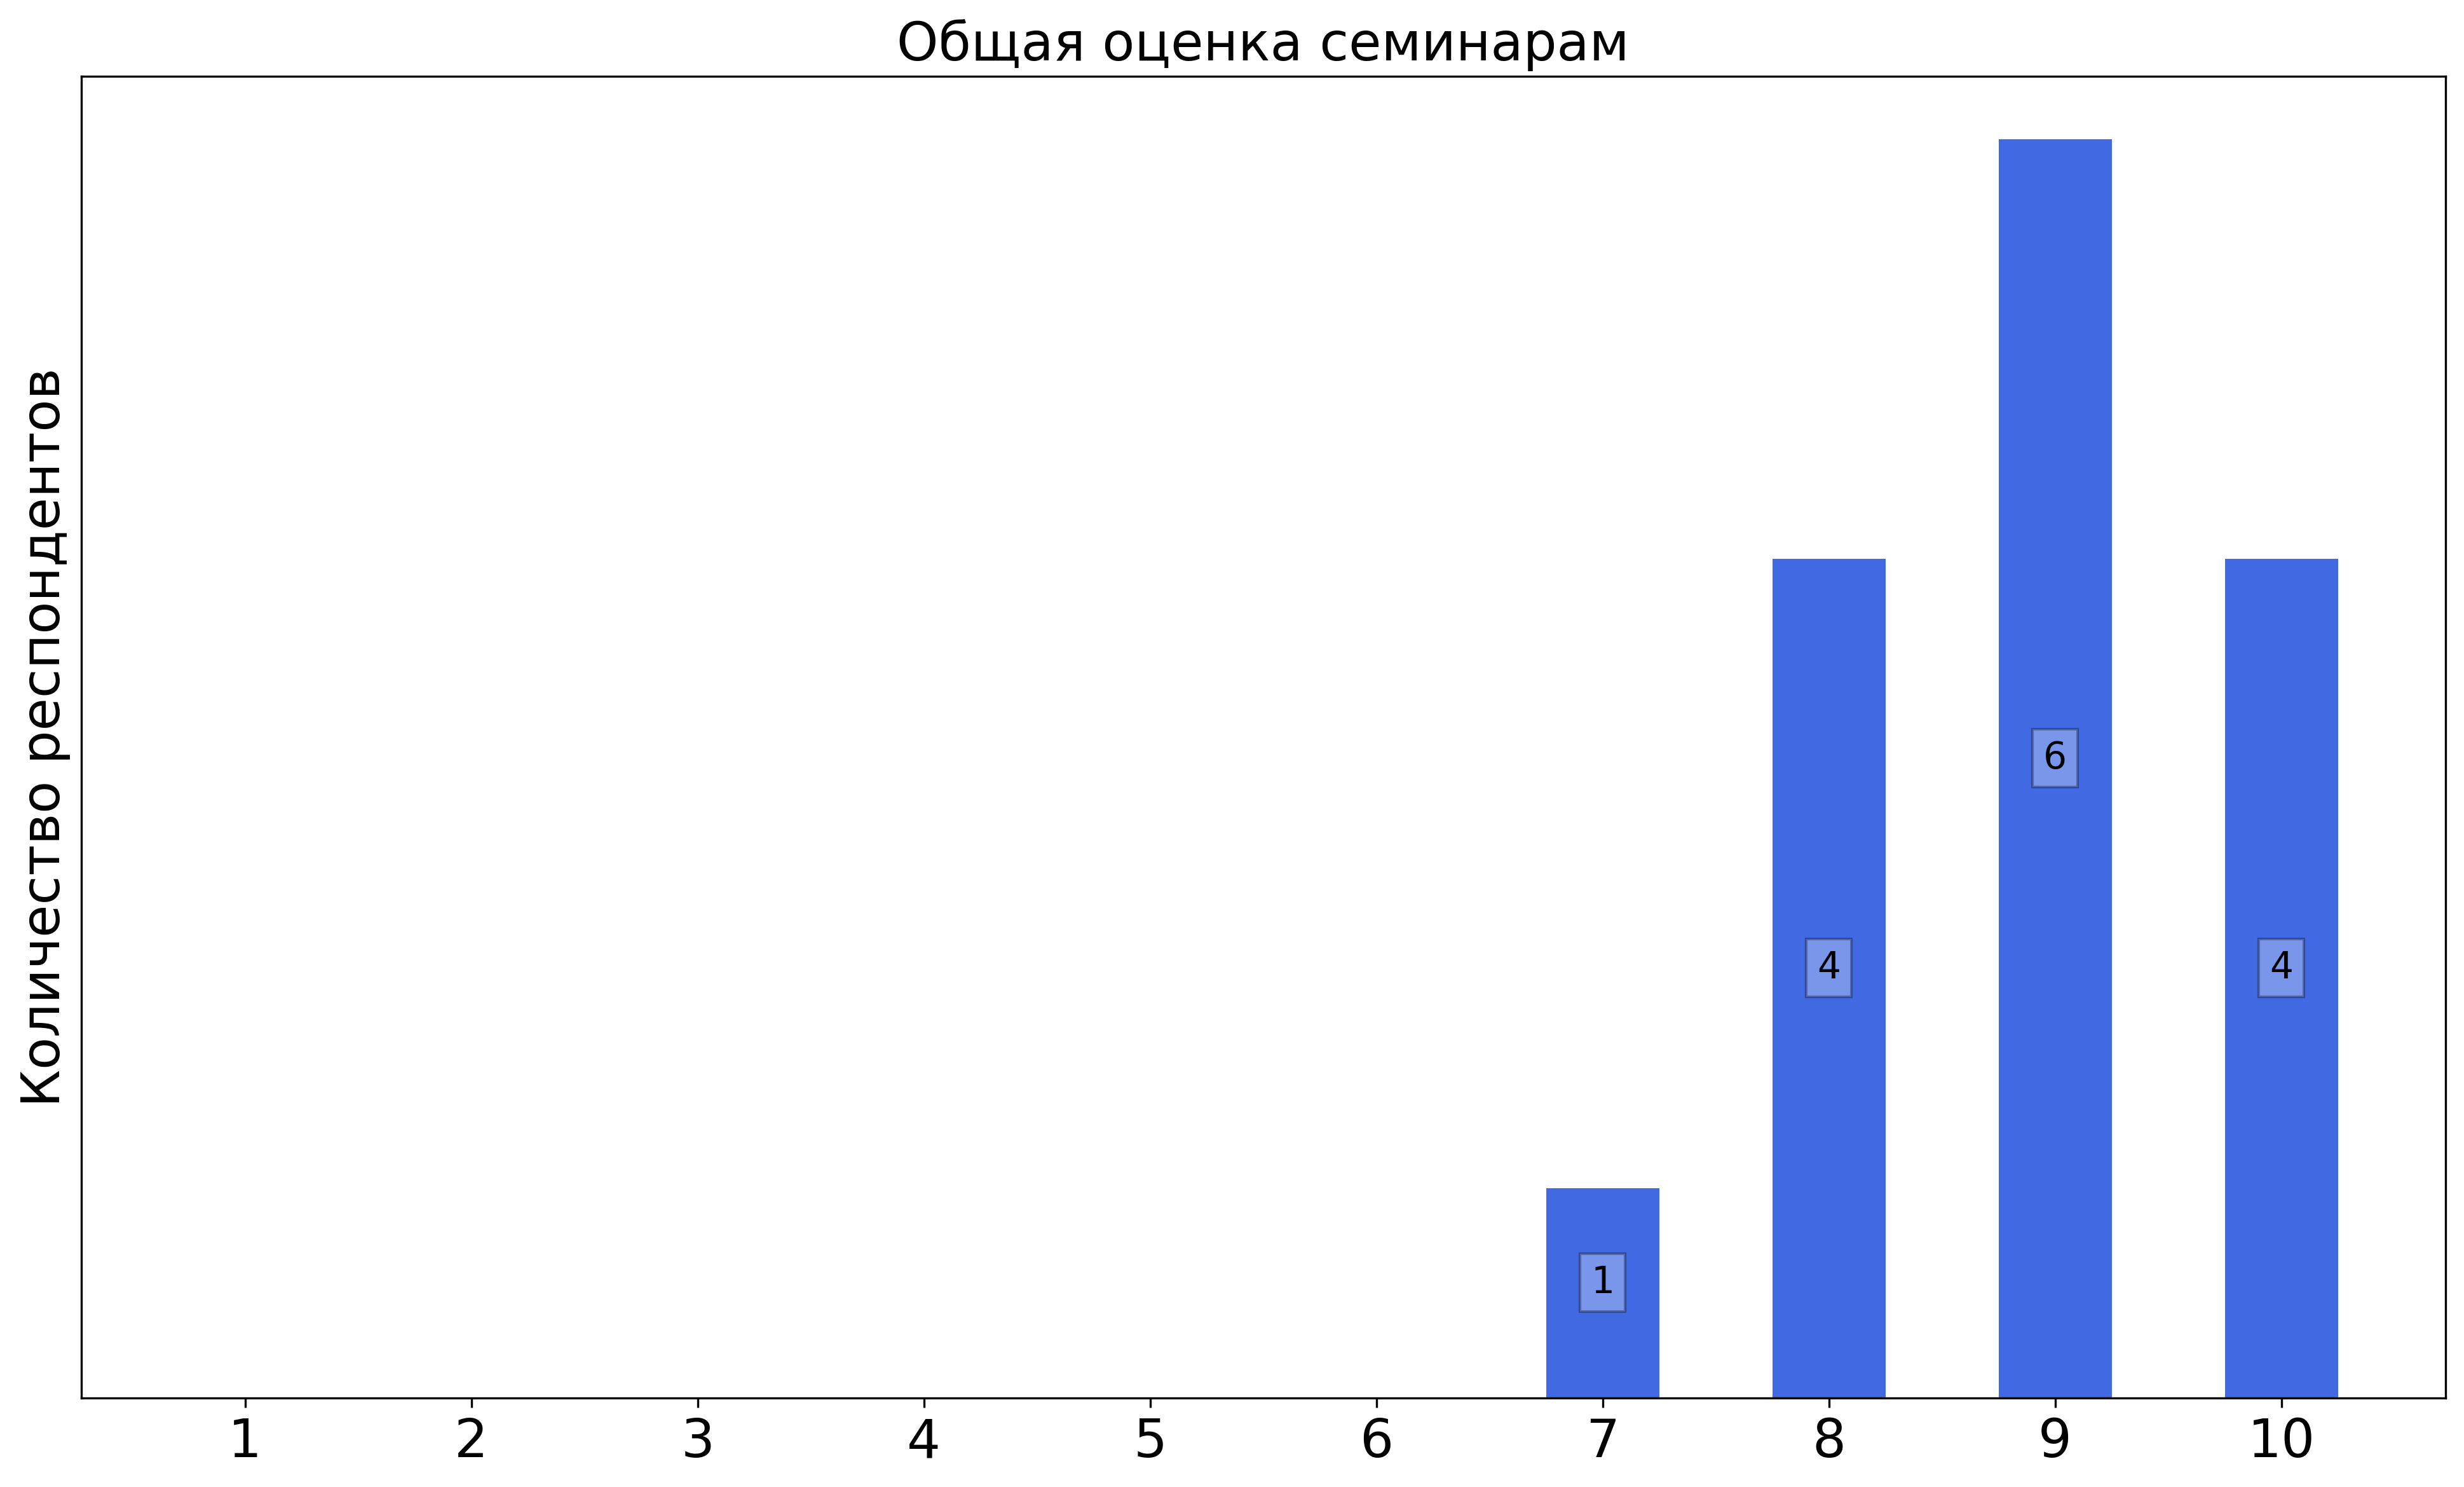
\includegraphics[width=\textwidth]{images/1 course/Математический анализ/seminarists-marks-Знаменская Л.Н.-3.png}
			\end{subfigure}	
			\caption{Оценки респондентов о качестве преподавания семинаров}
		\end{figure}

		\textbf{Комментарии студентов о семинаристе\protect\footnote{сохранены оригинальные орфография и пунктуация}}
			\begin{commentbox} 
				Не понравилось то, что совсем мало времени на подумать и зачастую стоя у доски ты просто пишешь под диктовку преподавателя. Это единственная претензия, остальное отлично 
			\end{commentbox} 
		
			\begin{commentbox} 
				То же самое, что и на лекциях. См. комментарий о лекторе 
			\end{commentbox} 
		
			\begin{commentbox} 
				в целом хорошо 
			\end{commentbox} 
		
			\begin{commentbox} 
				Хорошие полезные семинары, но были моменты, когда не очень понятно. В том числе и после ответов на вопросы. 
			\end{commentbox} 

					
	\subsubsection{Отзыв студентов о семинарах. Семинарист: Каржеманов И.В.}
		\begin{figure}[H]
			\centering
			\begin{subfigure}[b]{0.45\textwidth}
				\centering
				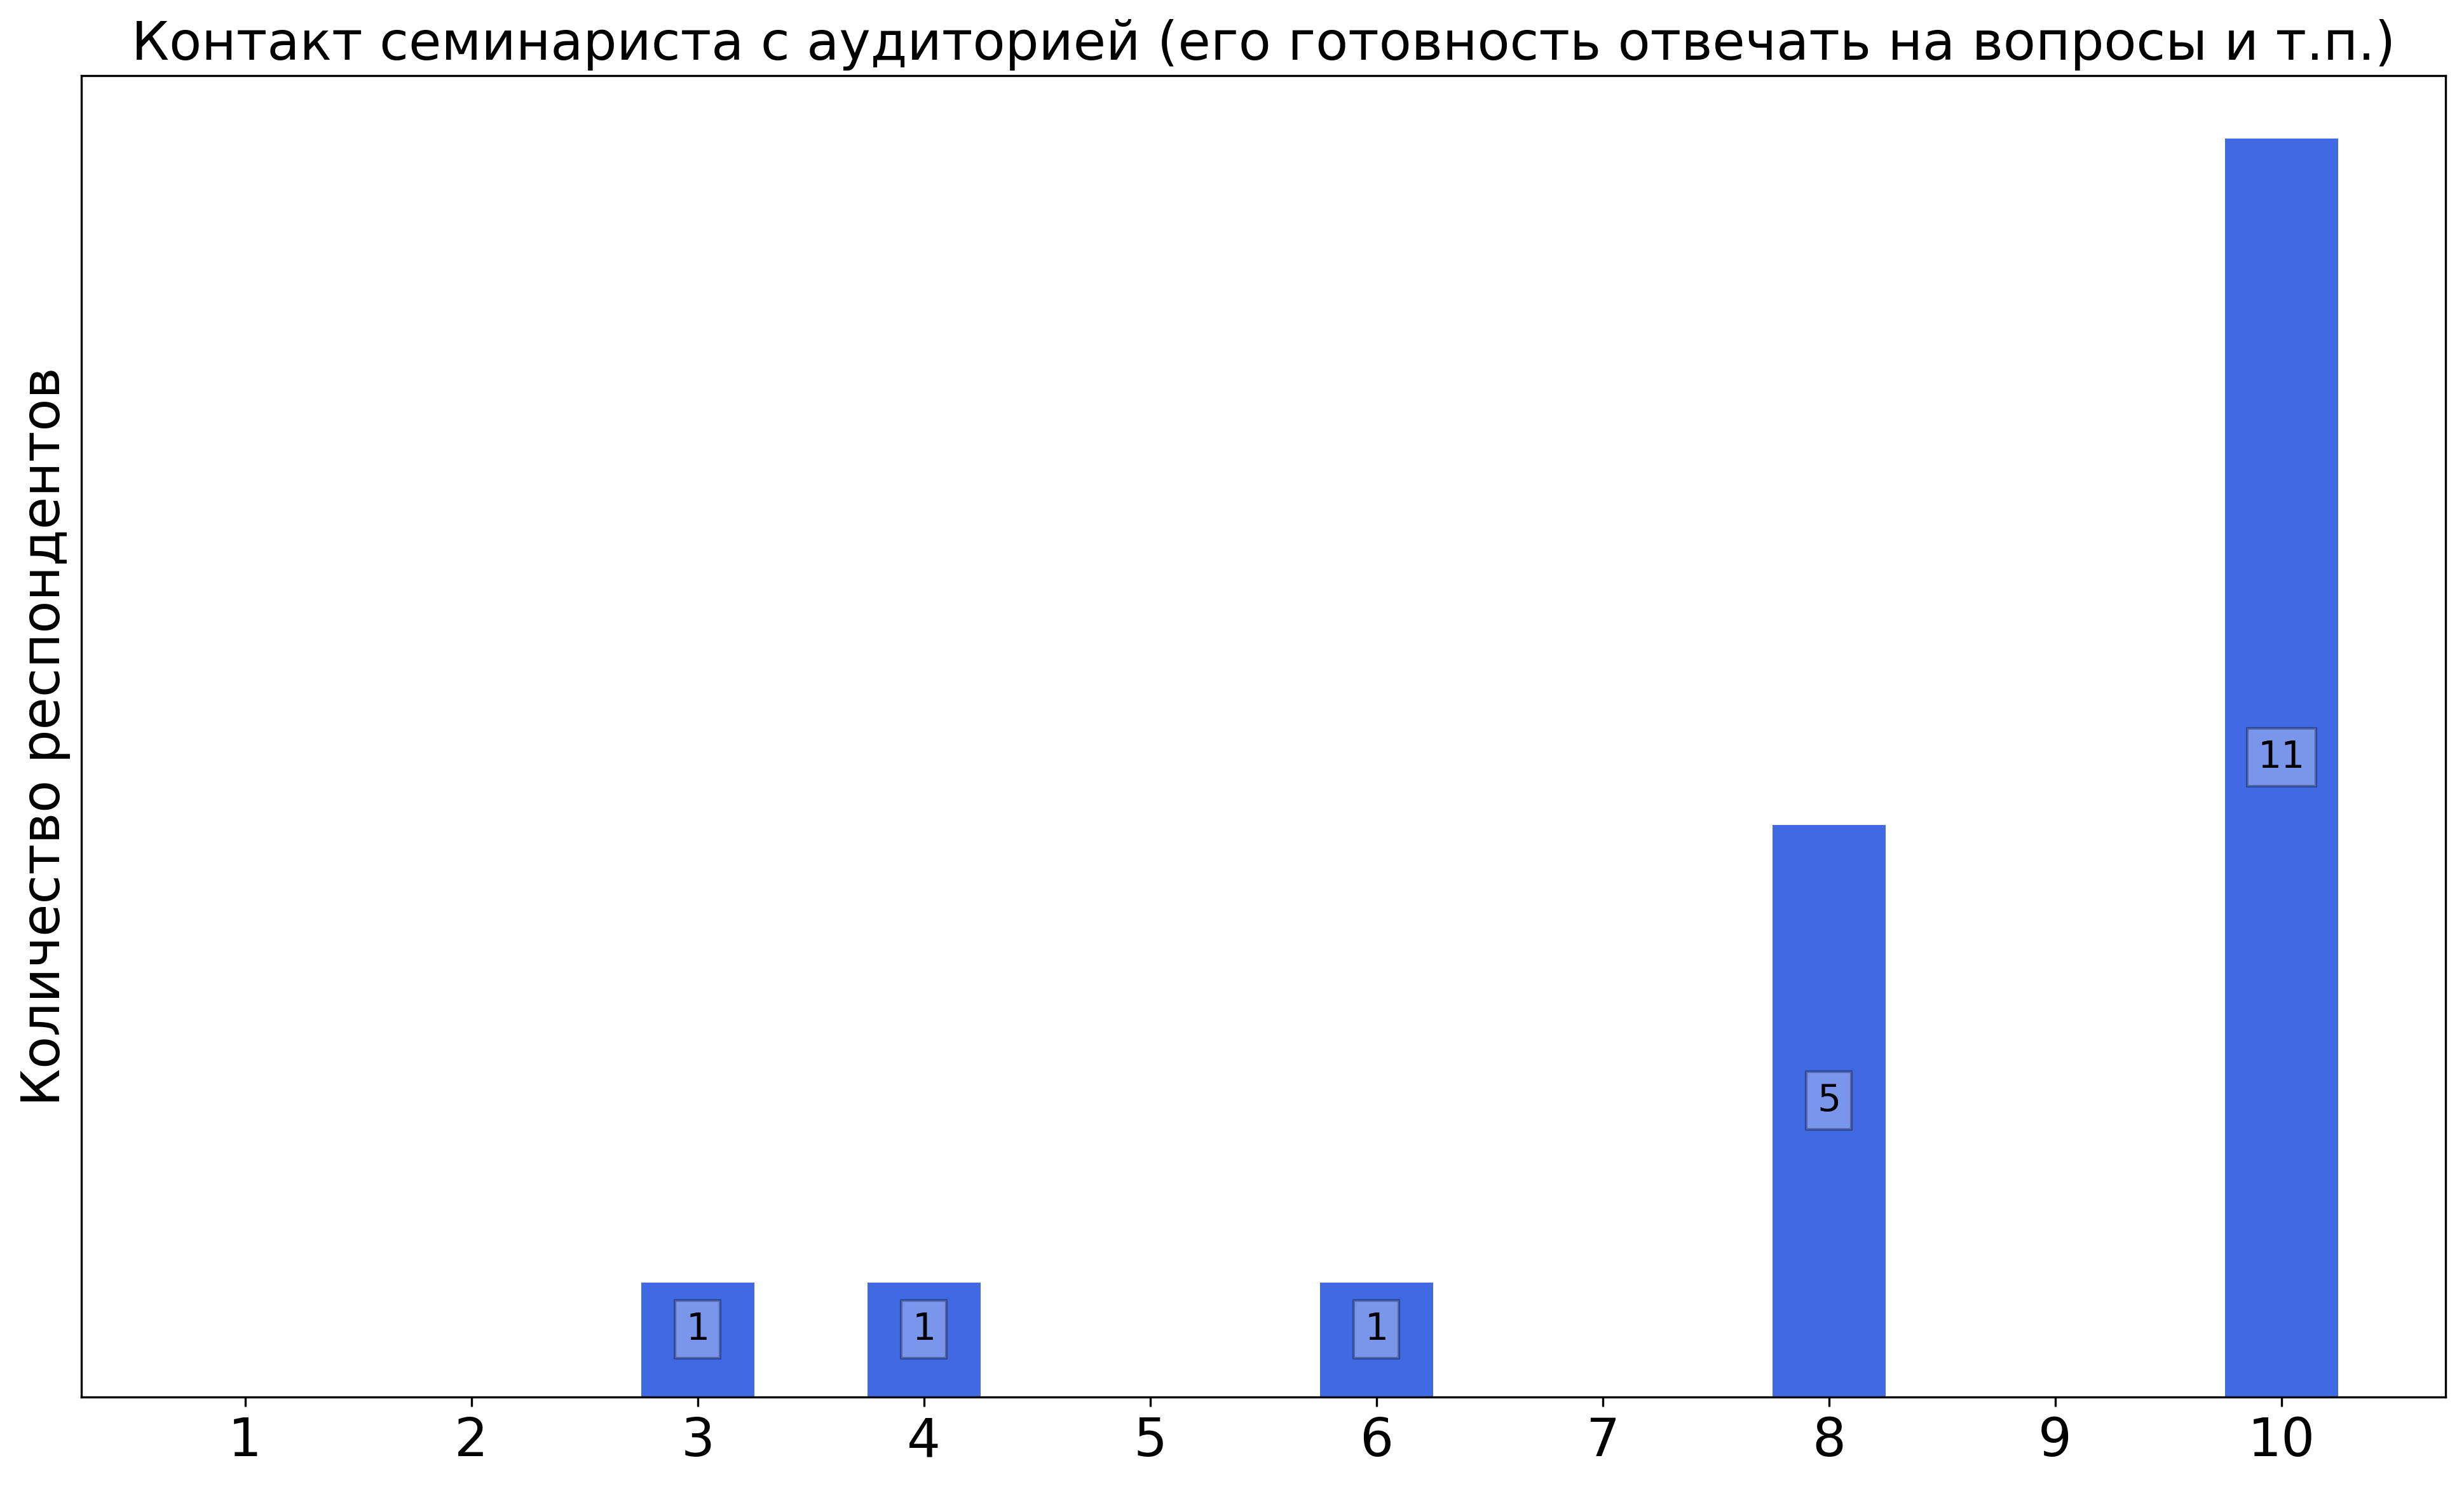
\includegraphics[width=\textwidth]{images/1 course/Математический анализ/seminarists-marks-Каржеманов И.В.-0.png}
			\end{subfigure}
			\begin{subfigure}[b]{0.45\textwidth}
				\centering
				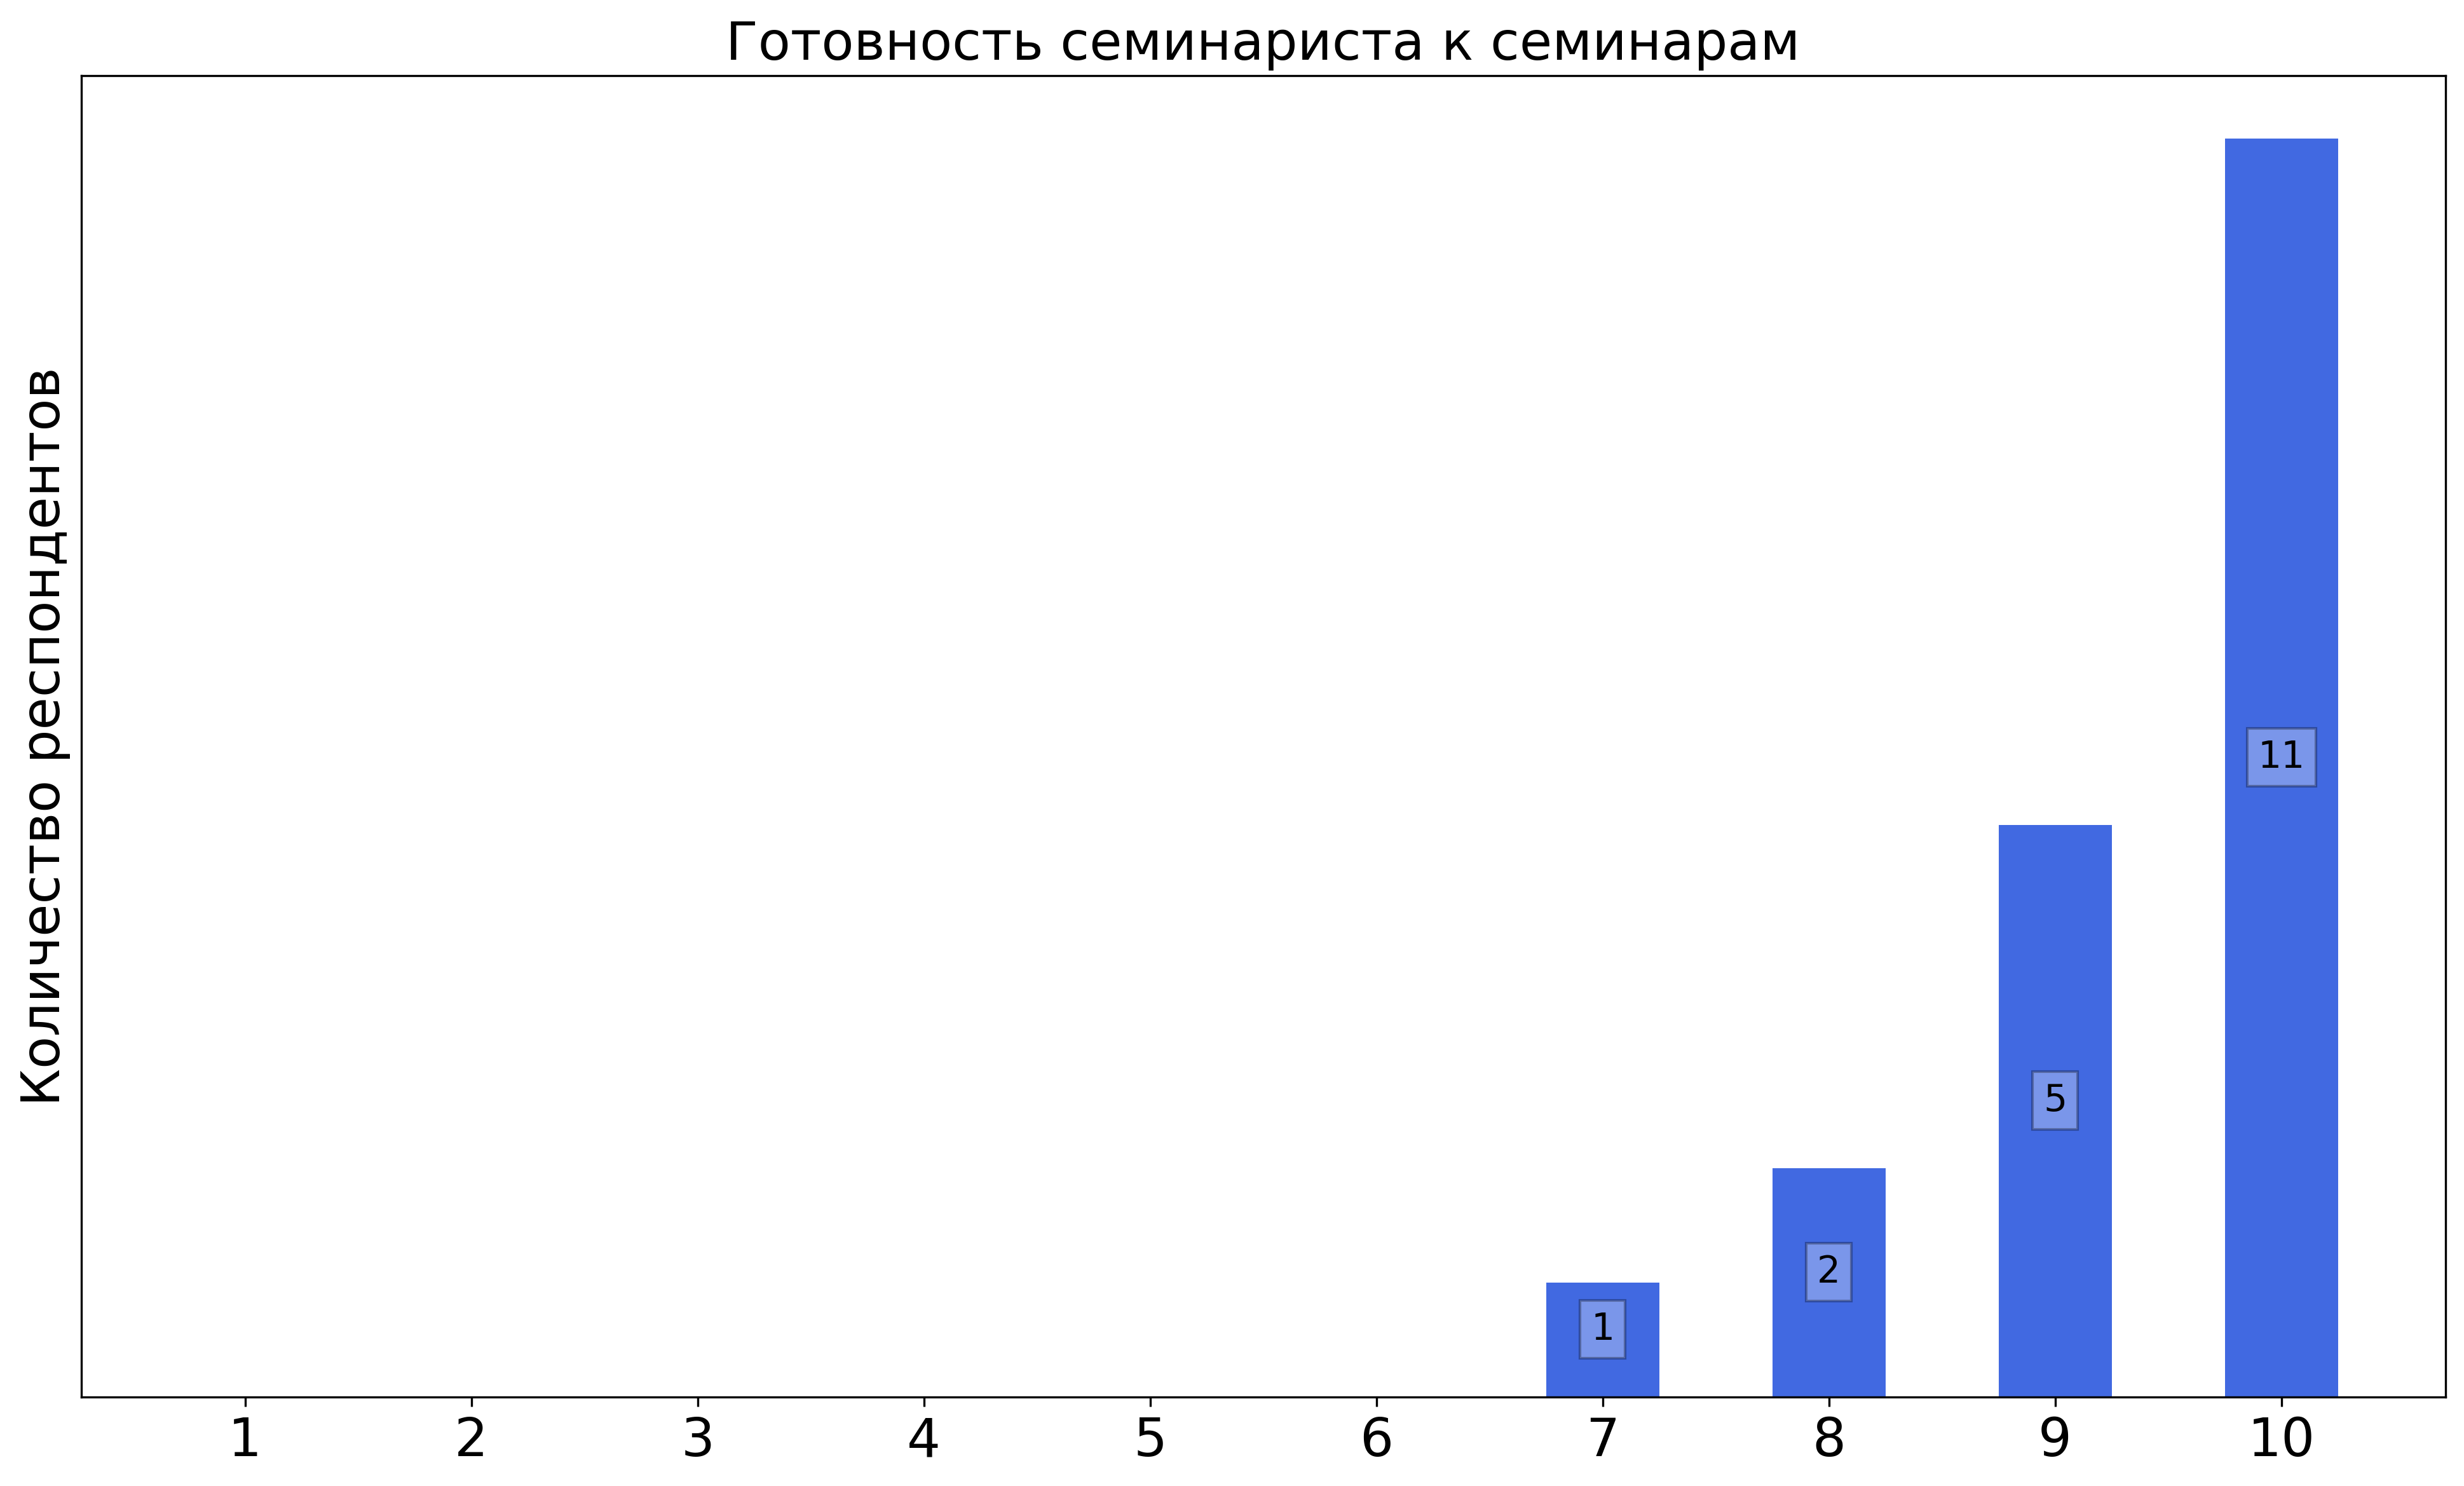
\includegraphics[width=\textwidth]{images/1 course/Математический анализ/seminarists-marks-Каржеманов И.В.-1.png}
			\end{subfigure}
			\begin{subfigure}[b]{0.45\textwidth}
				\centering
				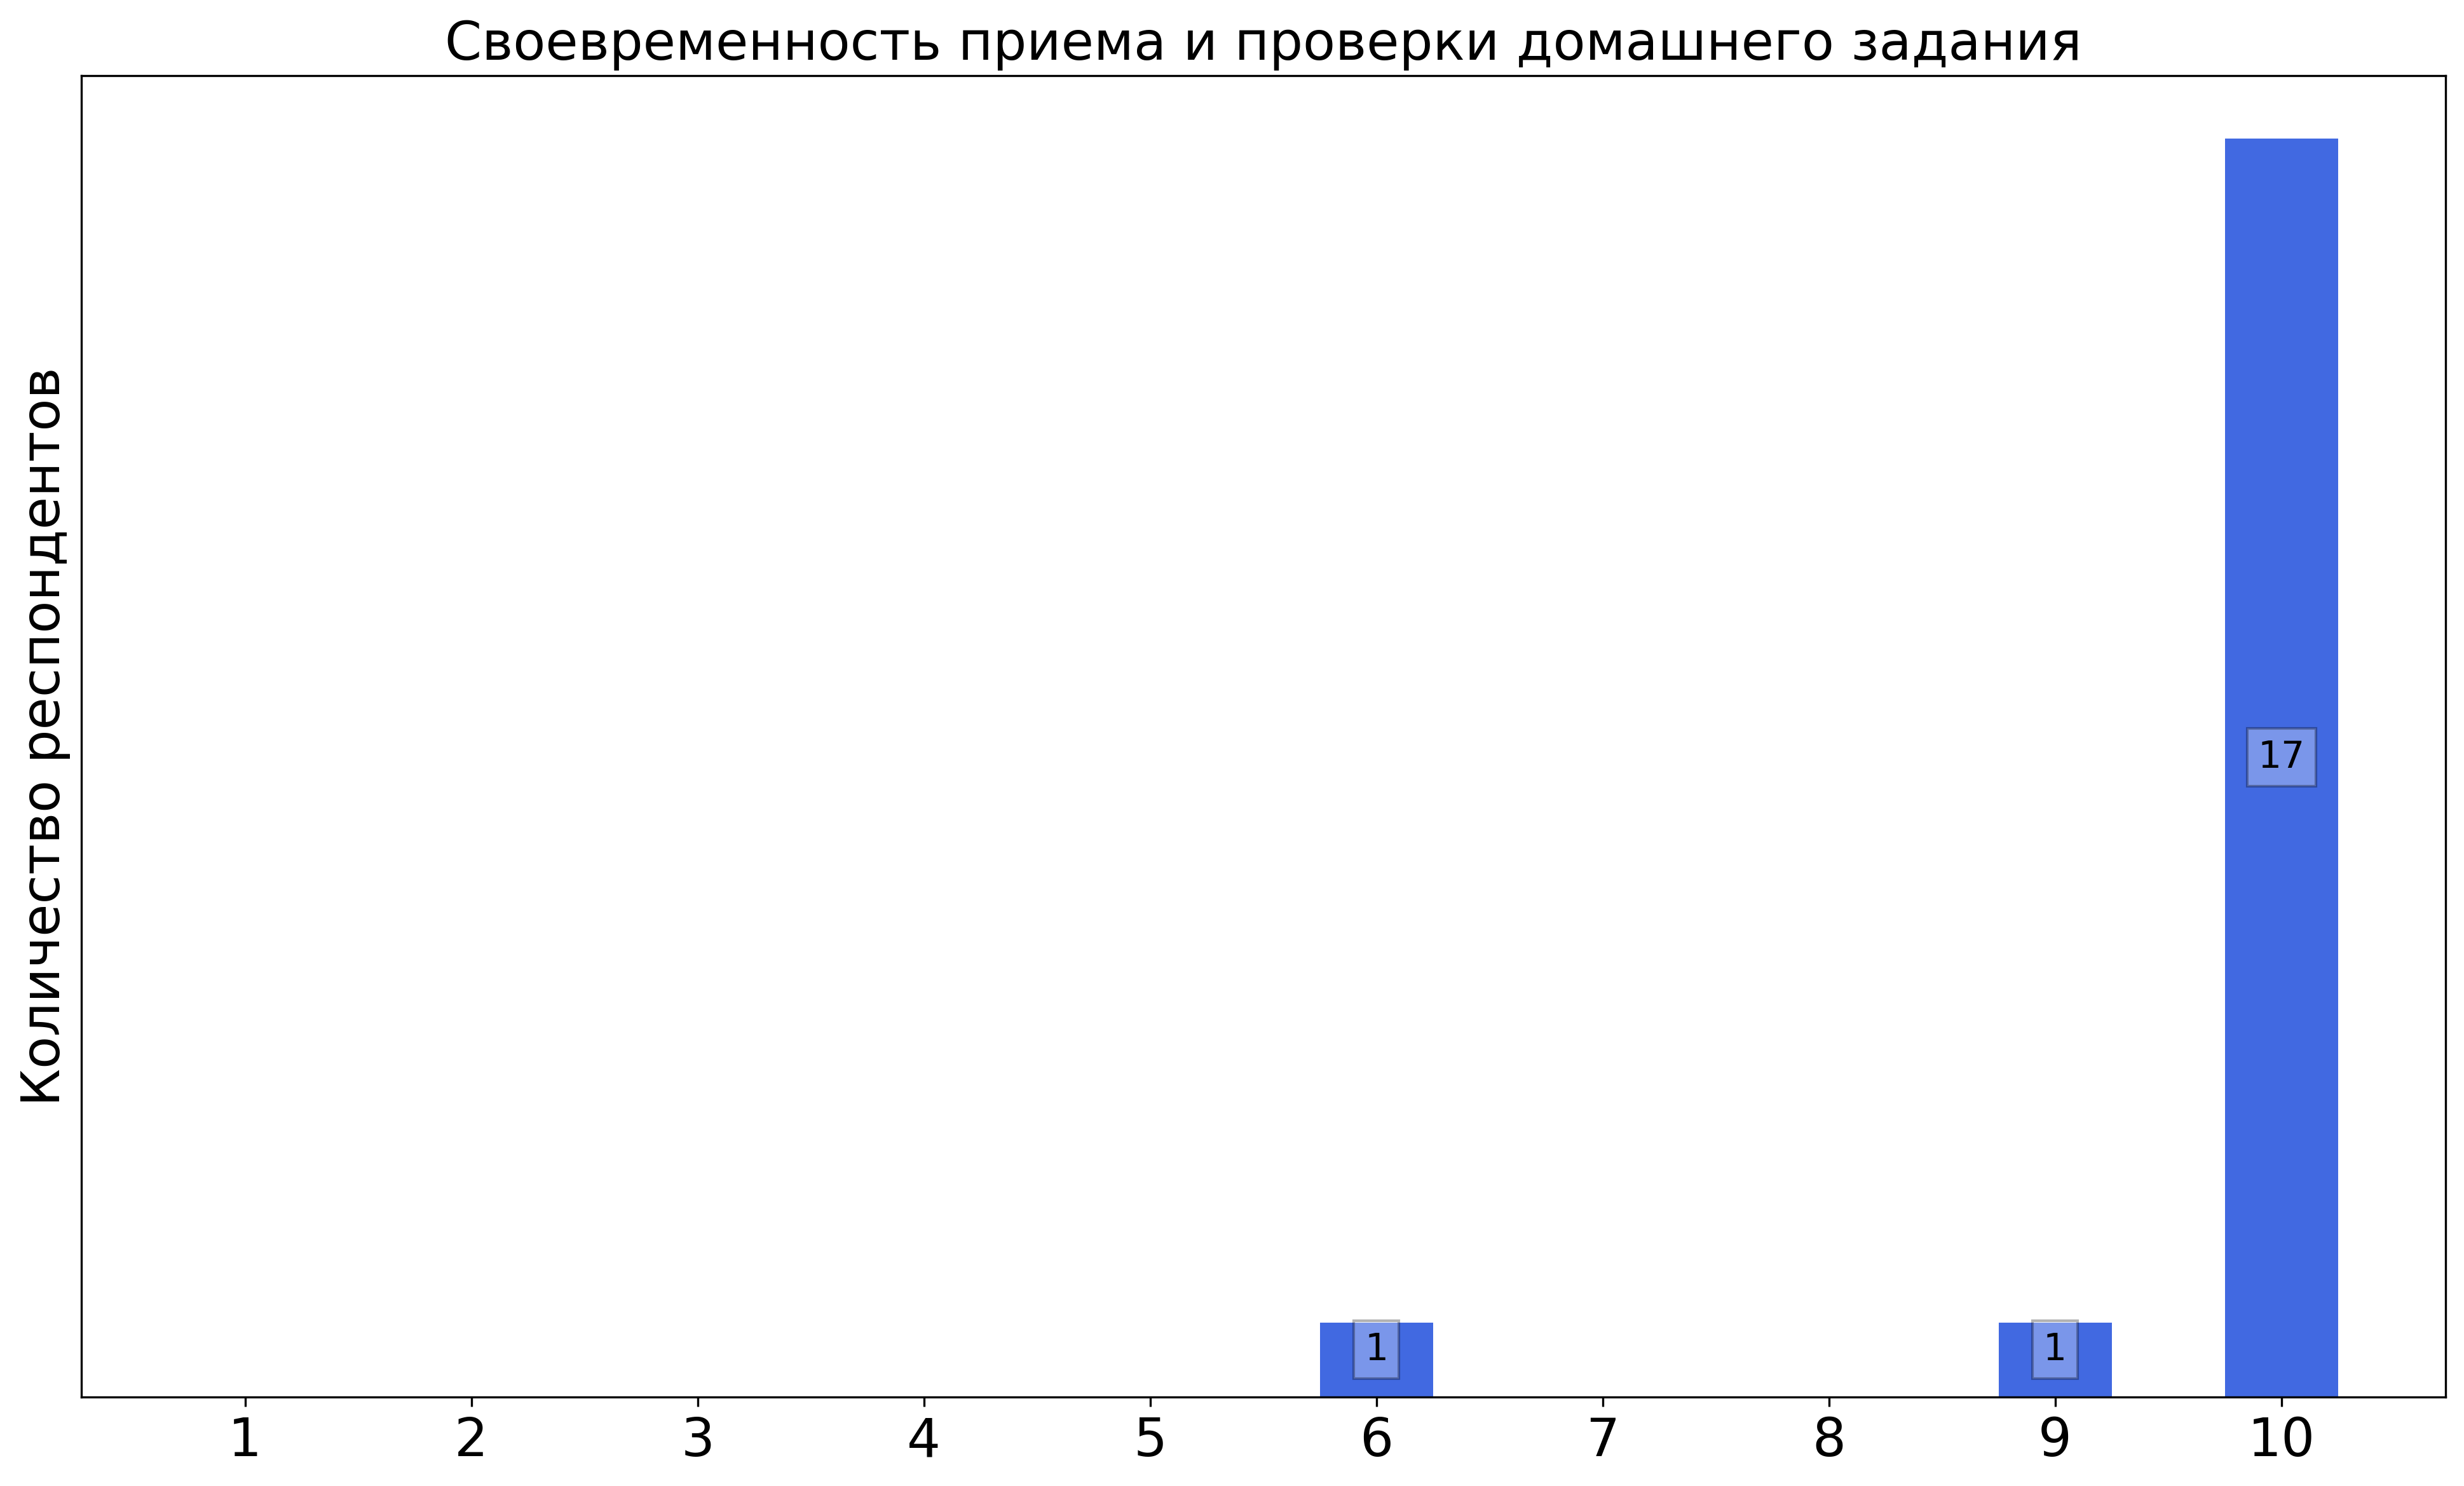
\includegraphics[width=\textwidth]{images/1 course/Математический анализ/seminarists-marks-Каржеманов И.В.-2.png}
			\end{subfigure}
			\begin{subfigure}[b]{0.45\textwidth}
				\centering
				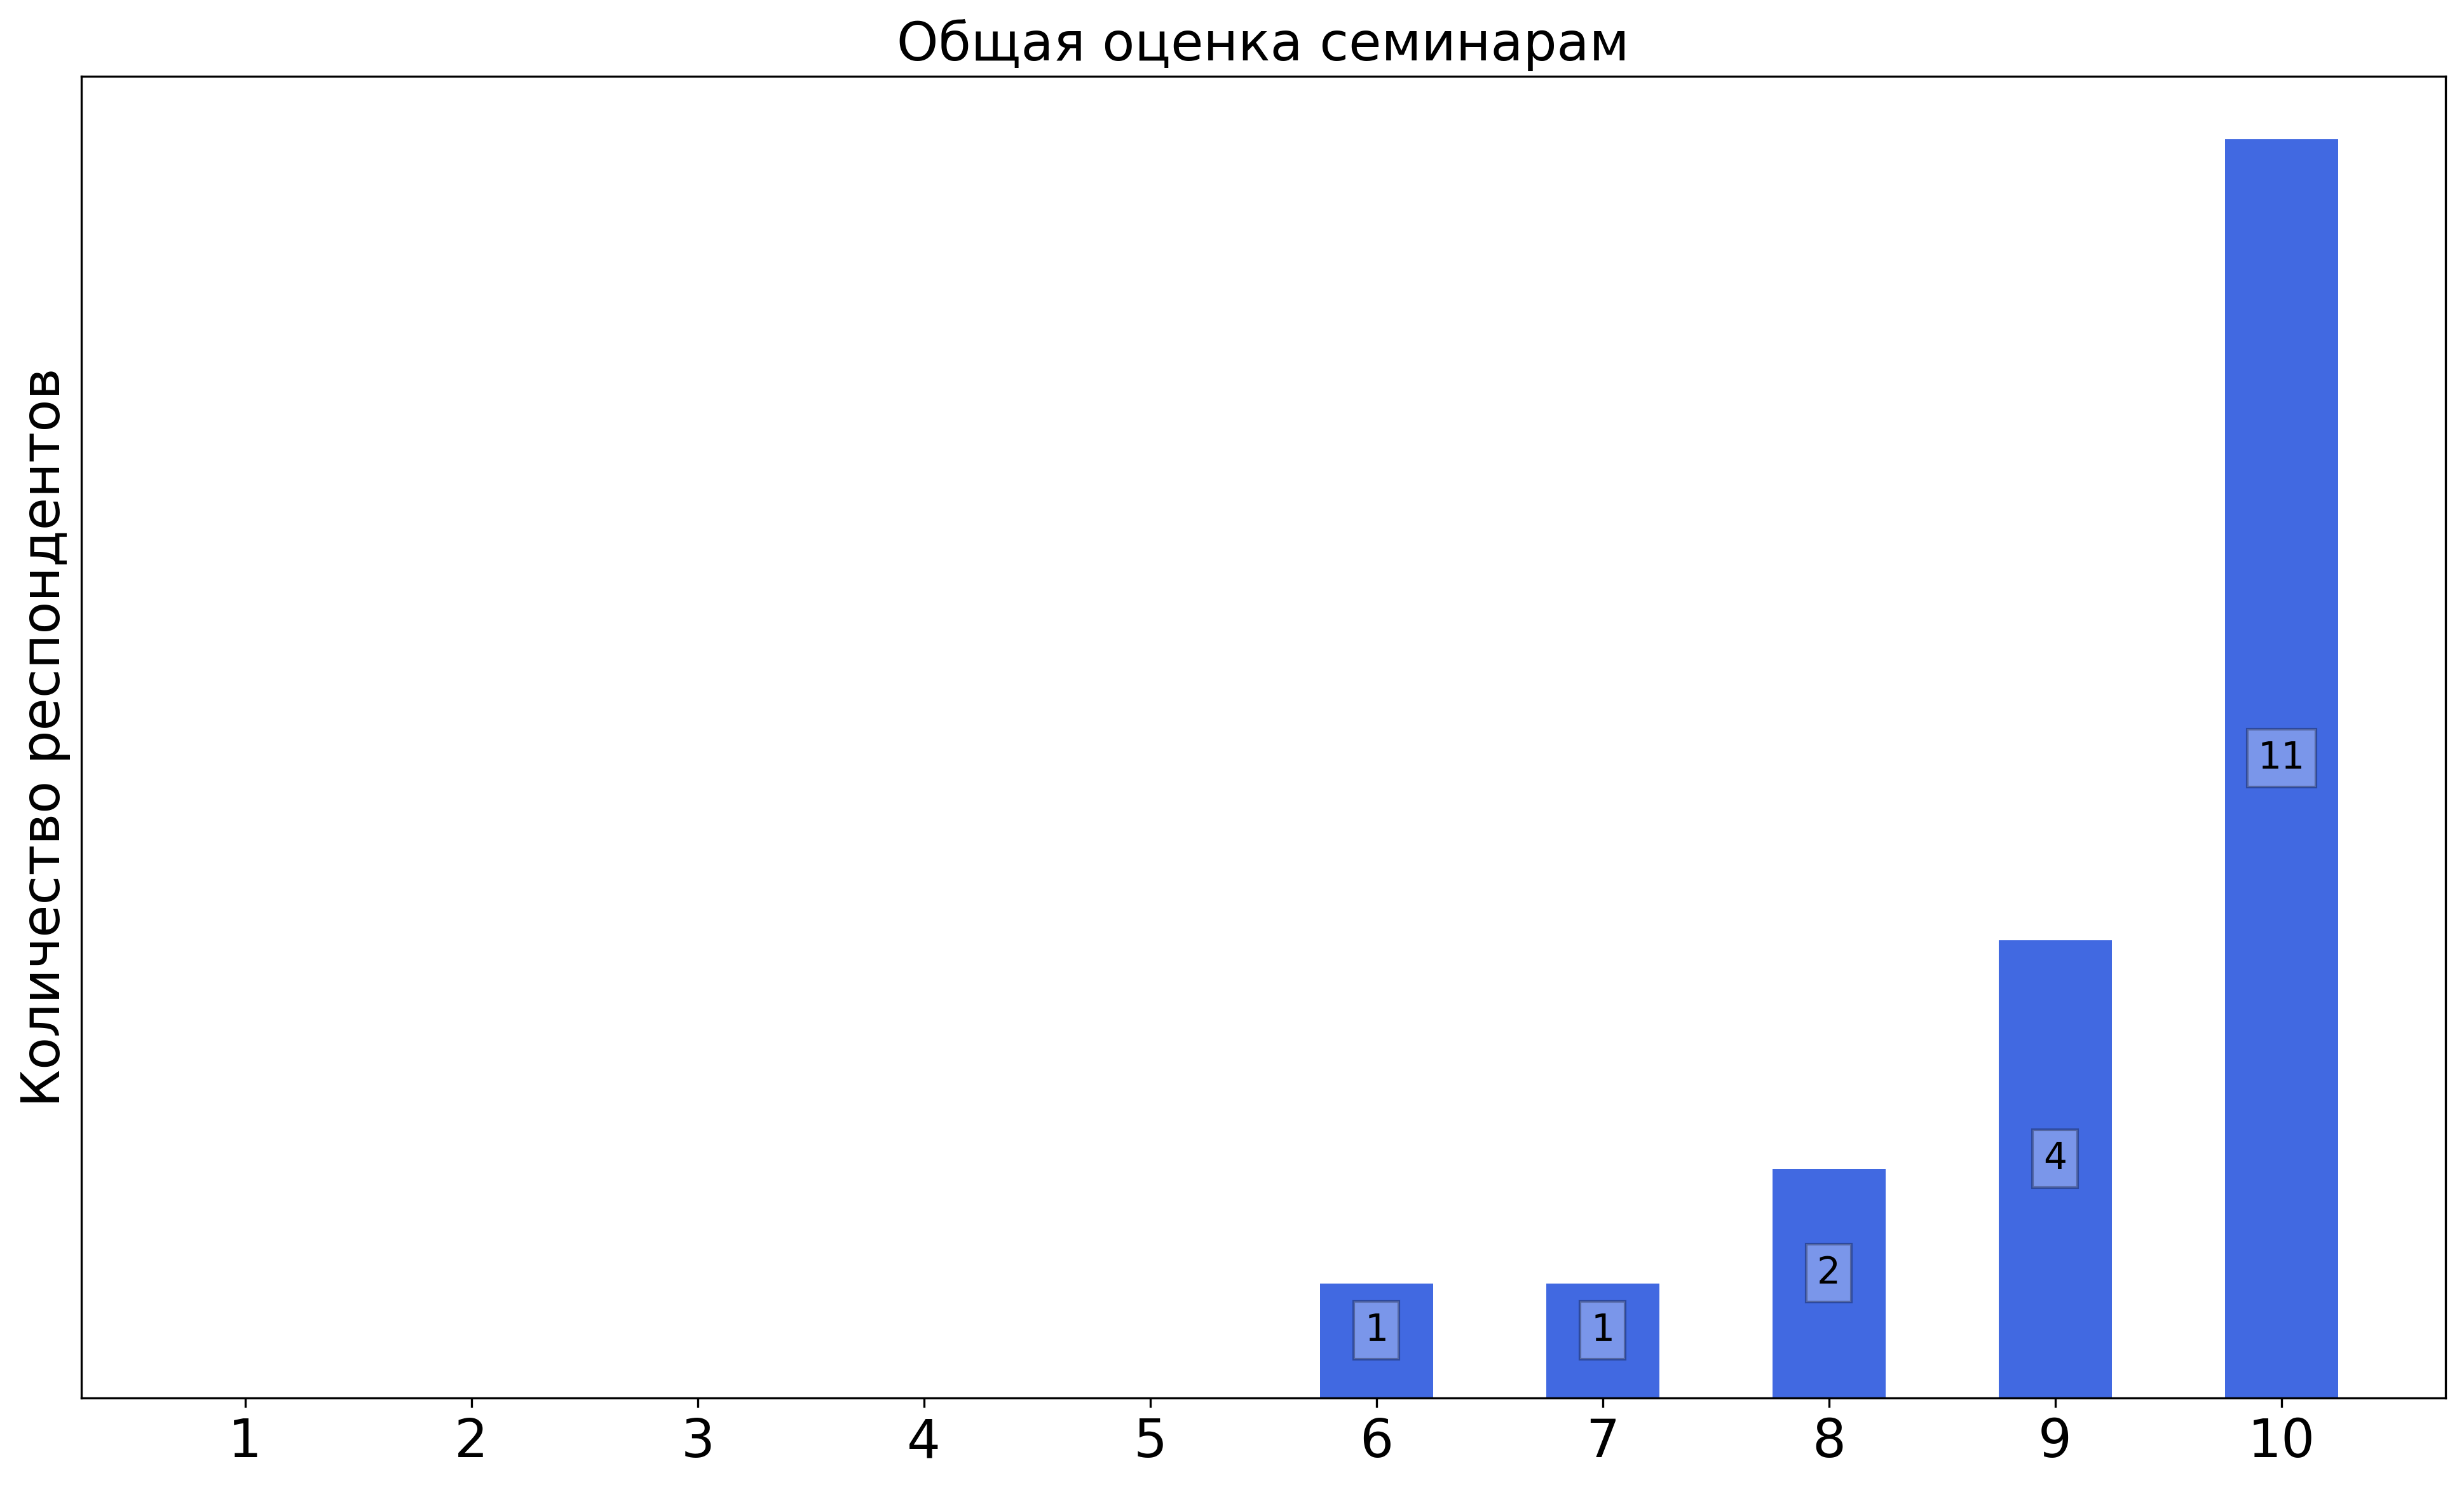
\includegraphics[width=\textwidth]{images/1 course/Математический анализ/seminarists-marks-Каржеманов И.В.-3.png}
			\end{subfigure}	
			\caption{Оценки респондентов о качестве преподавания семинаров}
		\end{figure}

		\textbf{Комментарии студентов о семинаристе\protect\footnote{сохранены оригинальные орфография и пунктуация}}
			\begin{commentbox} 
				Адекватный, если слушать внимательно. Старается поставить как можно больше брс 
			\end{commentbox} 
		
			\begin{commentbox} 
				Илья Вячеславович - отличный семинарист. Объясняет по-рабочекрестьянски, стремится, чтобы мы усвоили суть; лишнего со студентов не спрашивает, задания проверяет не слишком въедливо. Сам тщательно подбирает слова и со студентов требует того же. 
			\end{commentbox} 
		
			\begin{commentbox} 
				Очень крутой семинарист. Жестко все расшарит. Дает самое необходимое. Понятно и по делу. 
			\end{commentbox} 
		
			\begin{commentbox} 
				Крутой мужик  
			\end{commentbox} 
		
			\begin{commentbox} 
				невероятно харизматичный препод, лоялен на сдаче дз, отлично излагает материал 
			\end{commentbox}


	\subsubsection{Отзыв студентов о семинарах. Семинарист: Кондрашов О.В.}
		\begin{figure}[H]
			\centering
			\begin{subfigure}[b]{0.45\textwidth}
				\centering
				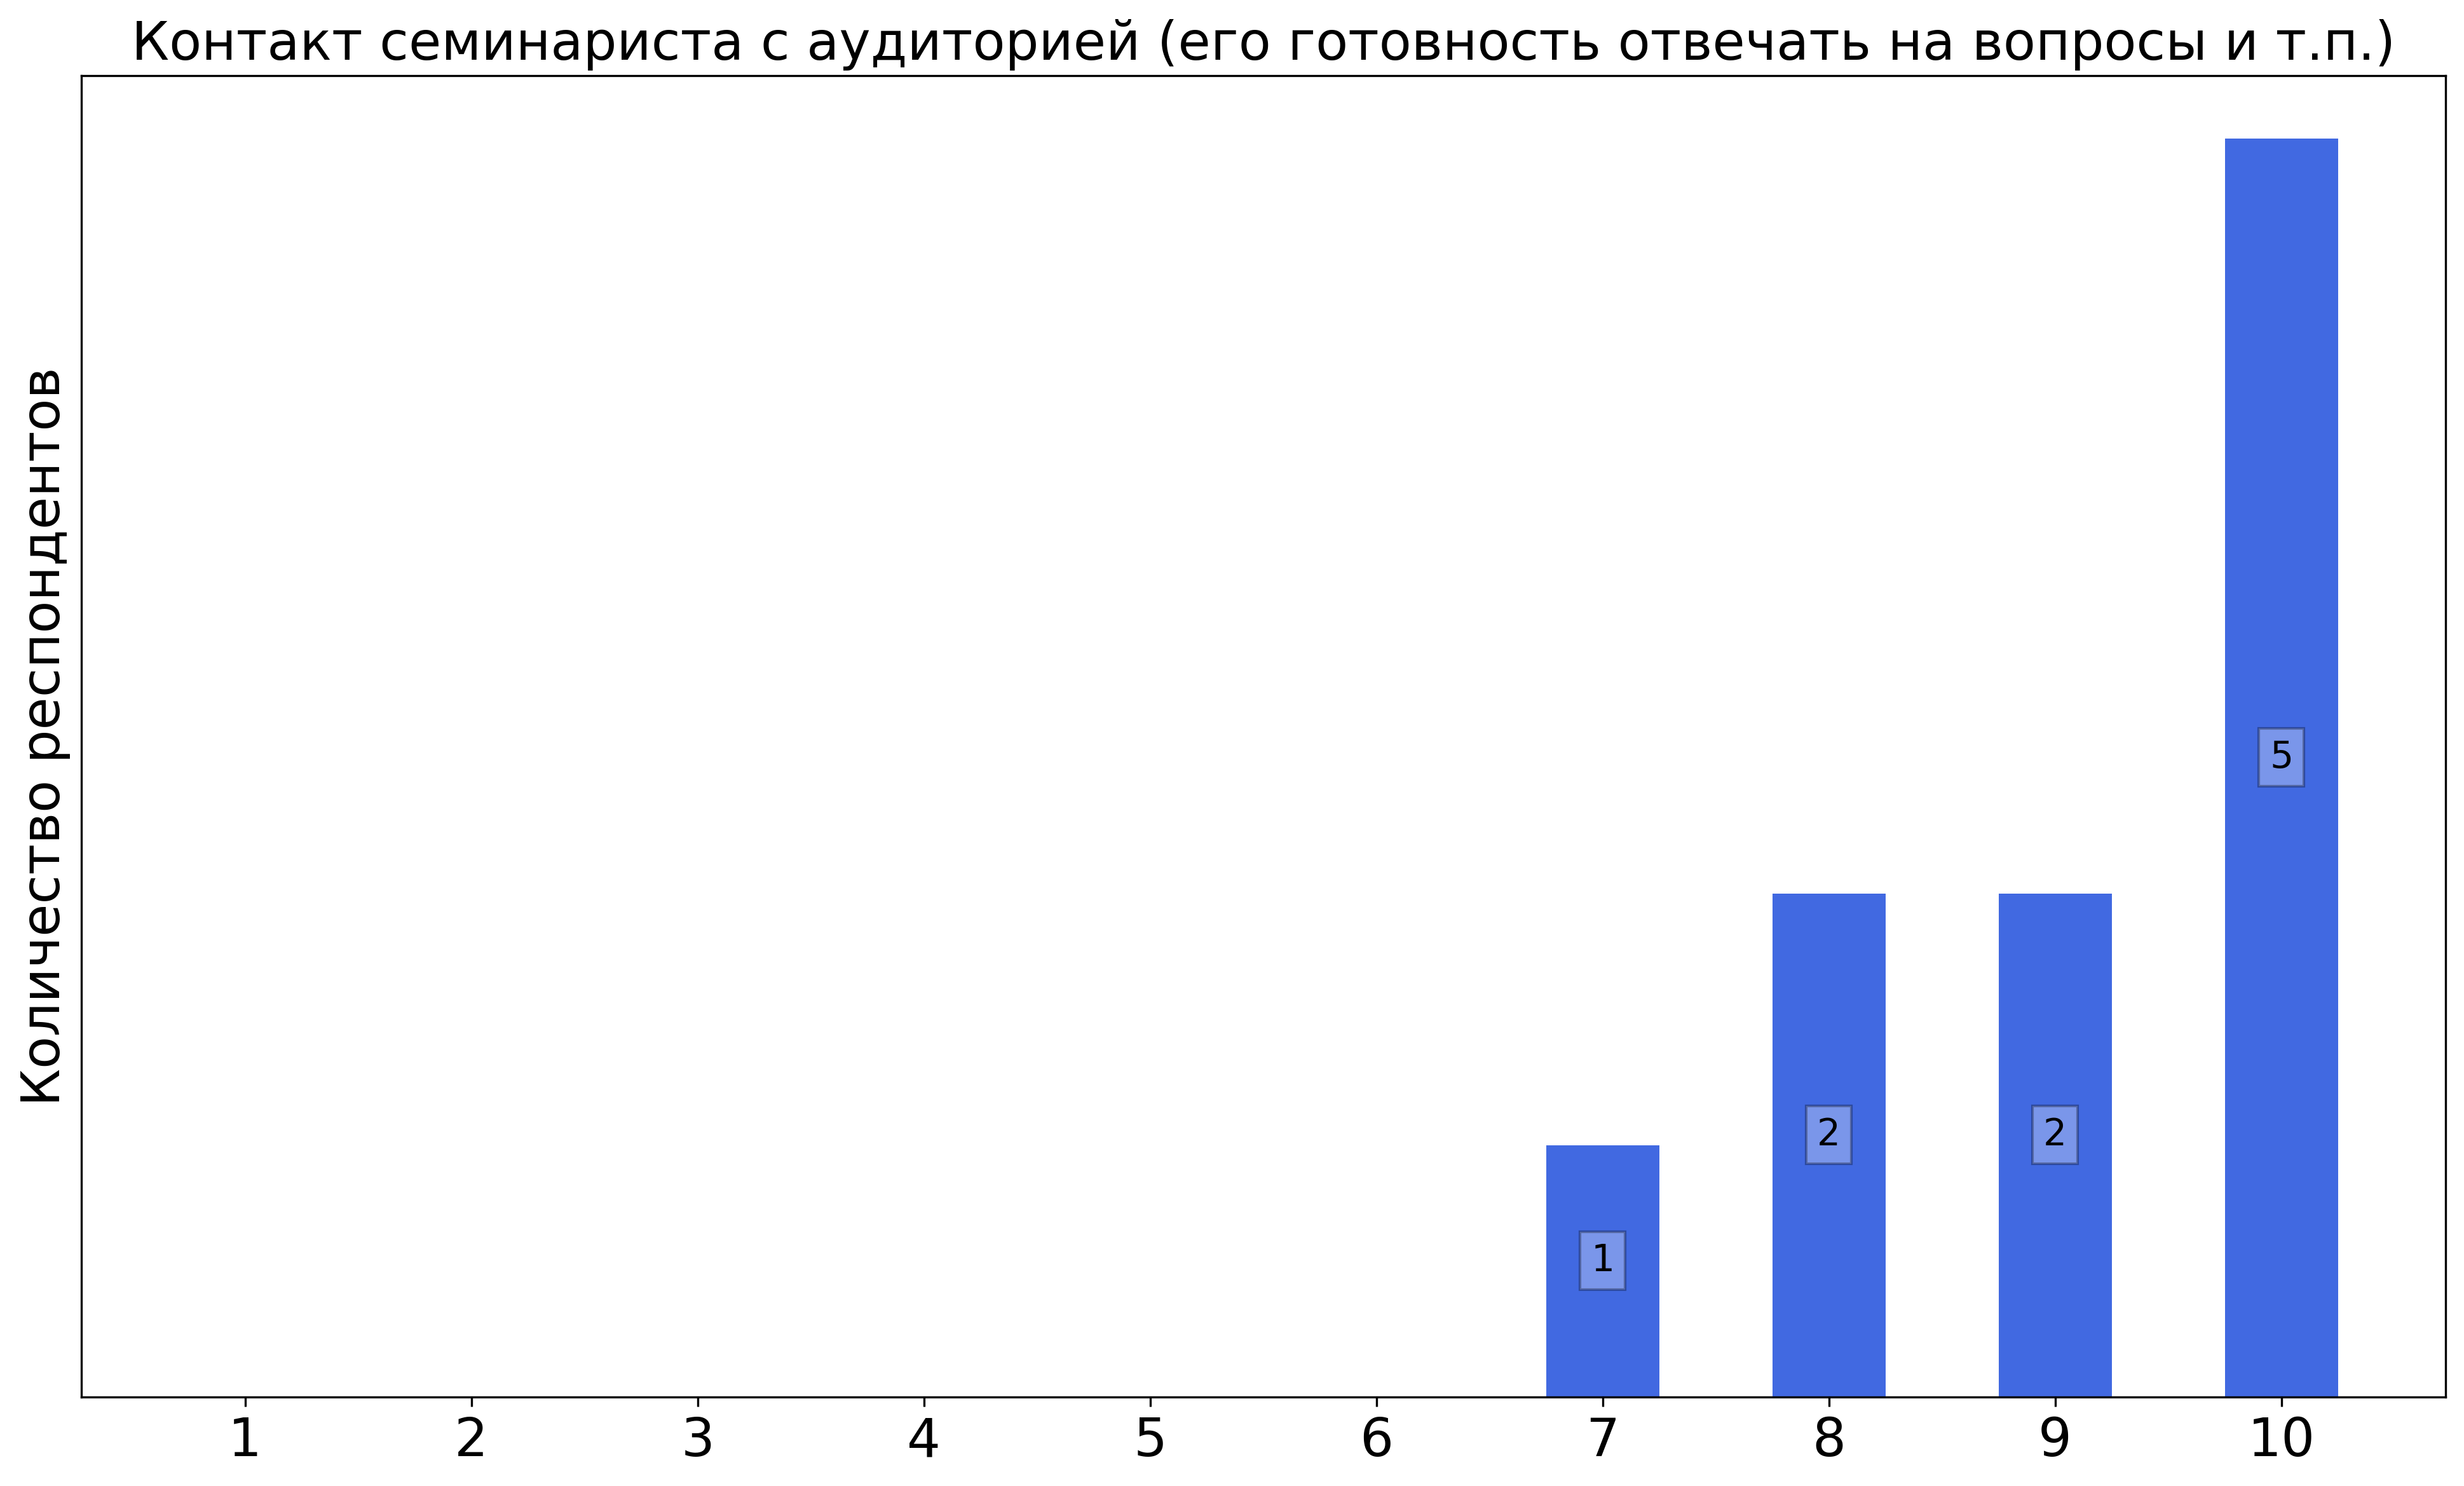
\includegraphics[width=\textwidth]{images/1 course/Математический анализ/seminarists-marks-Кондрашов О.В.-0.png}
			\end{subfigure}
			\begin{subfigure}[b]{0.45\textwidth}
				\centering
				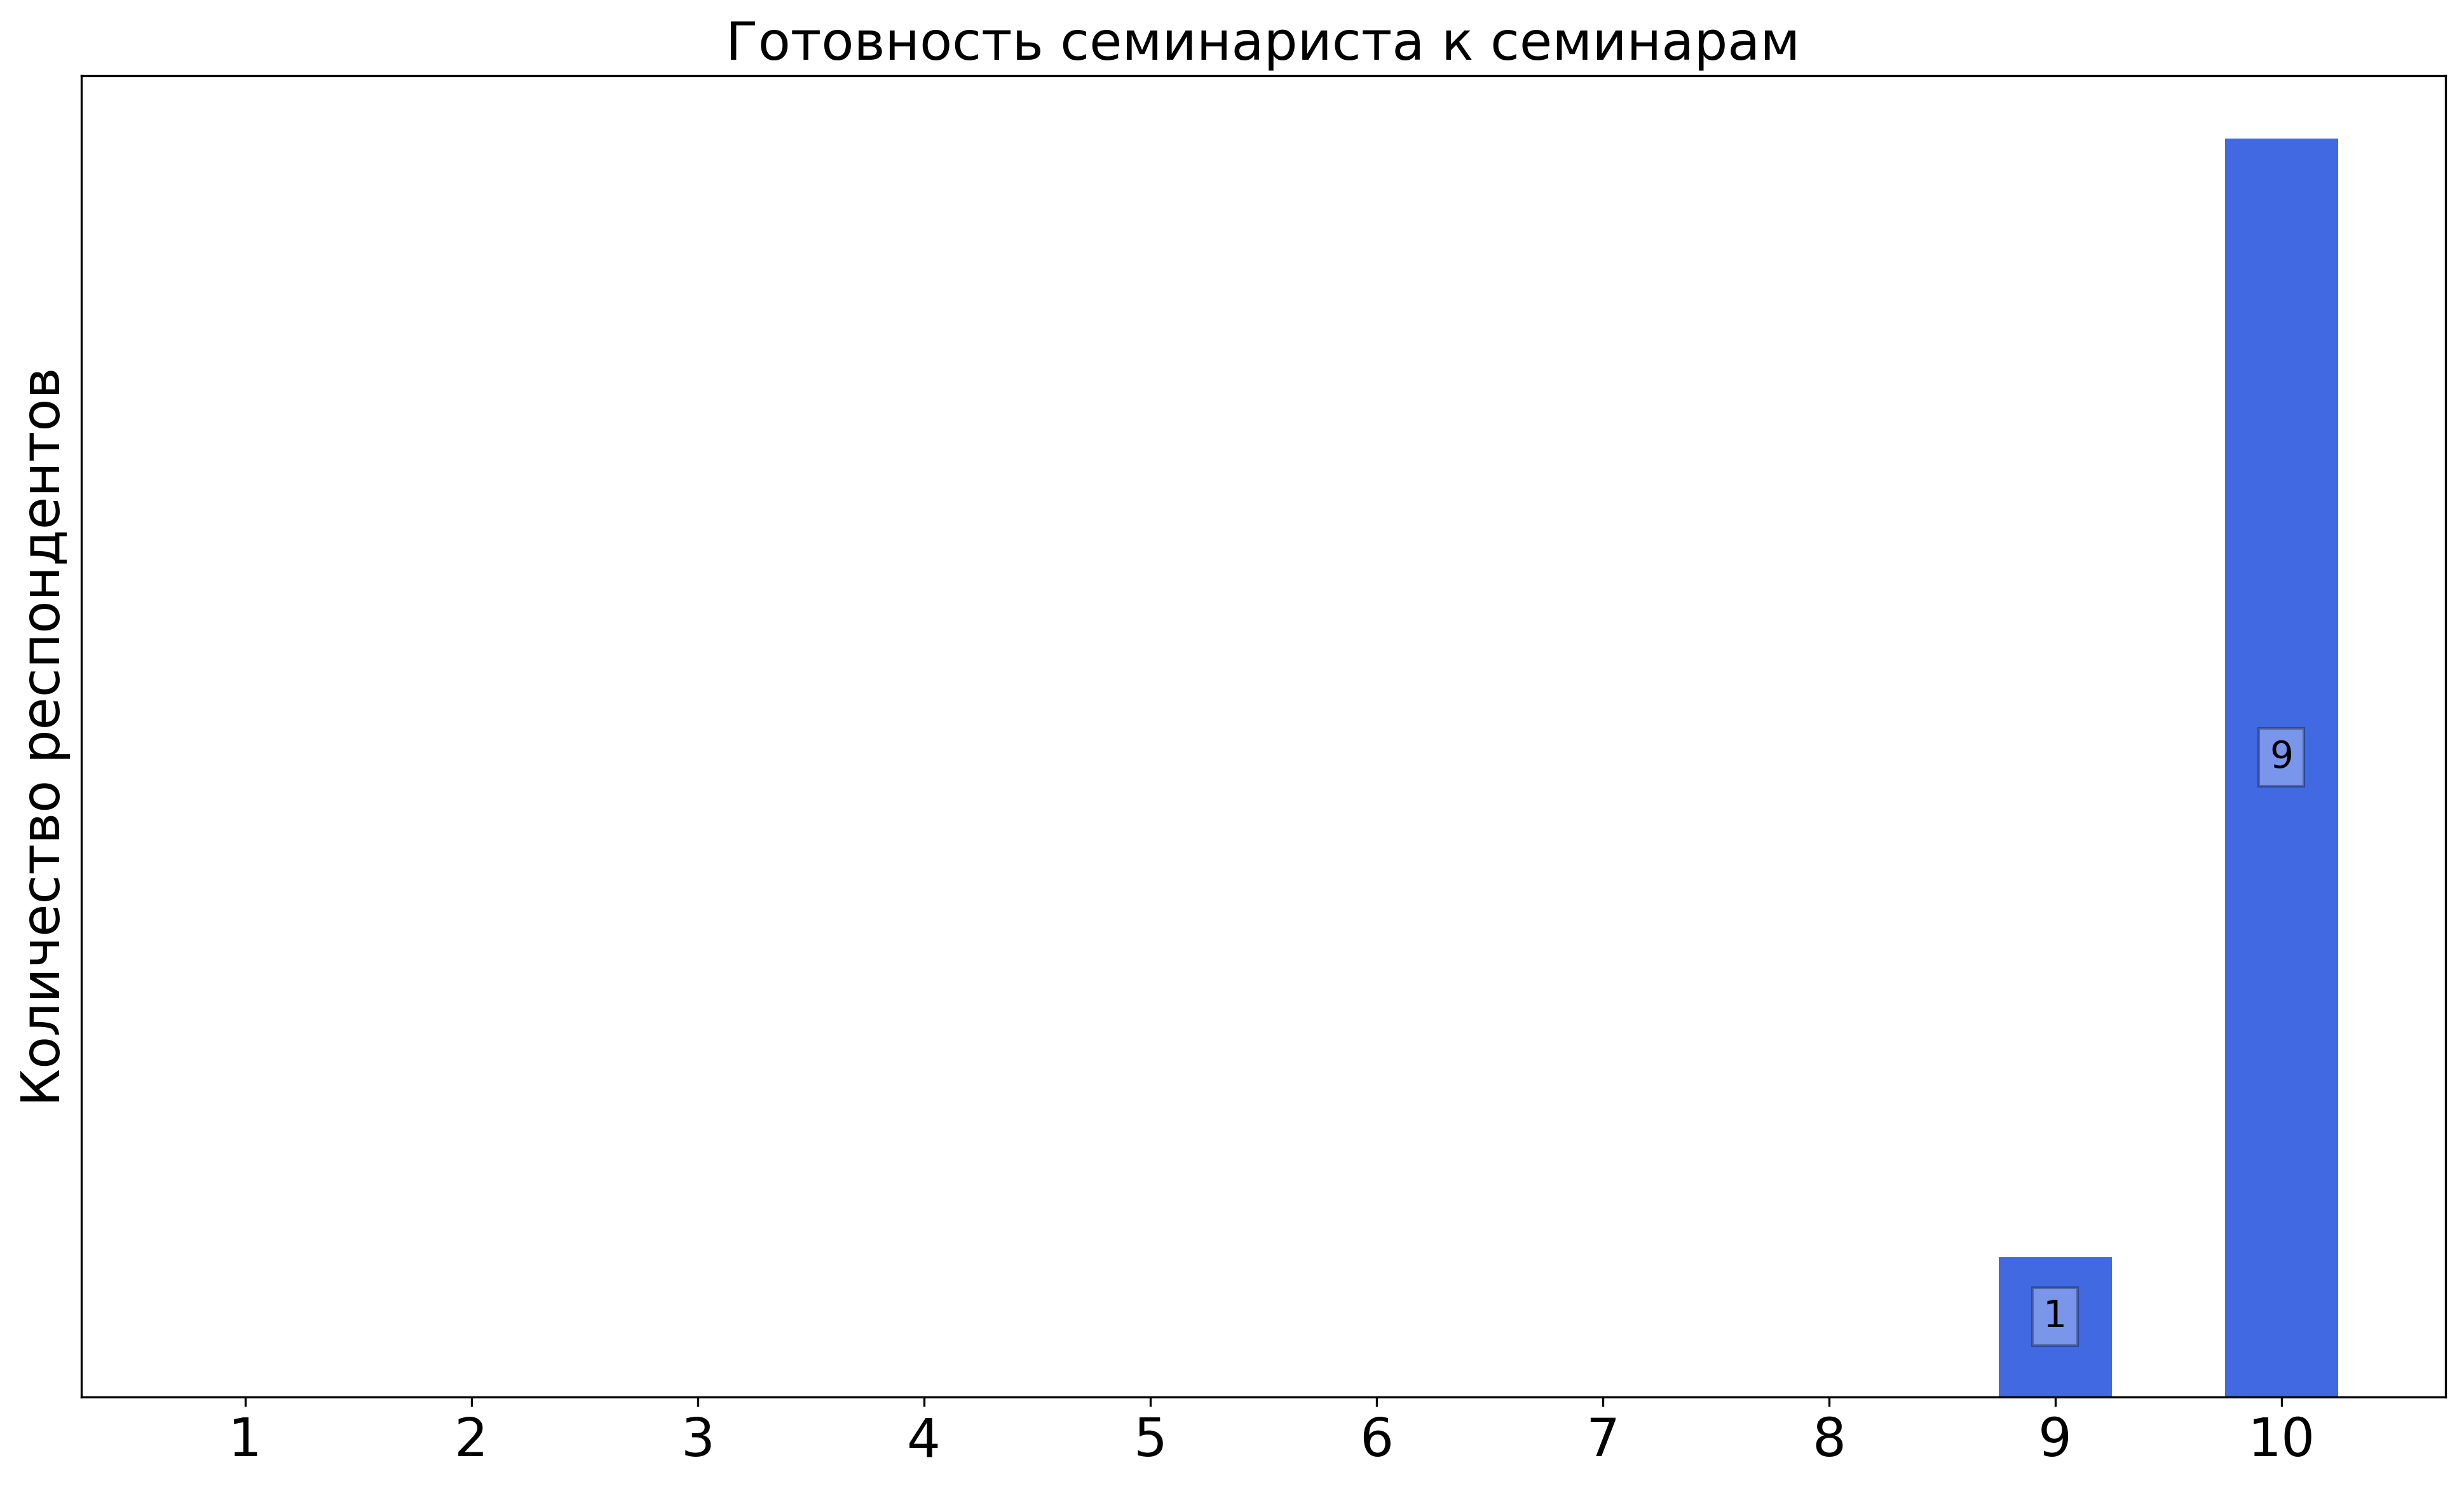
\includegraphics[width=\textwidth]{images/1 course/Математический анализ/seminarists-marks-Кондрашов О.В.-1.png}
			\end{subfigure}
			\begin{subfigure}[b]{0.45\textwidth}
				\centering
				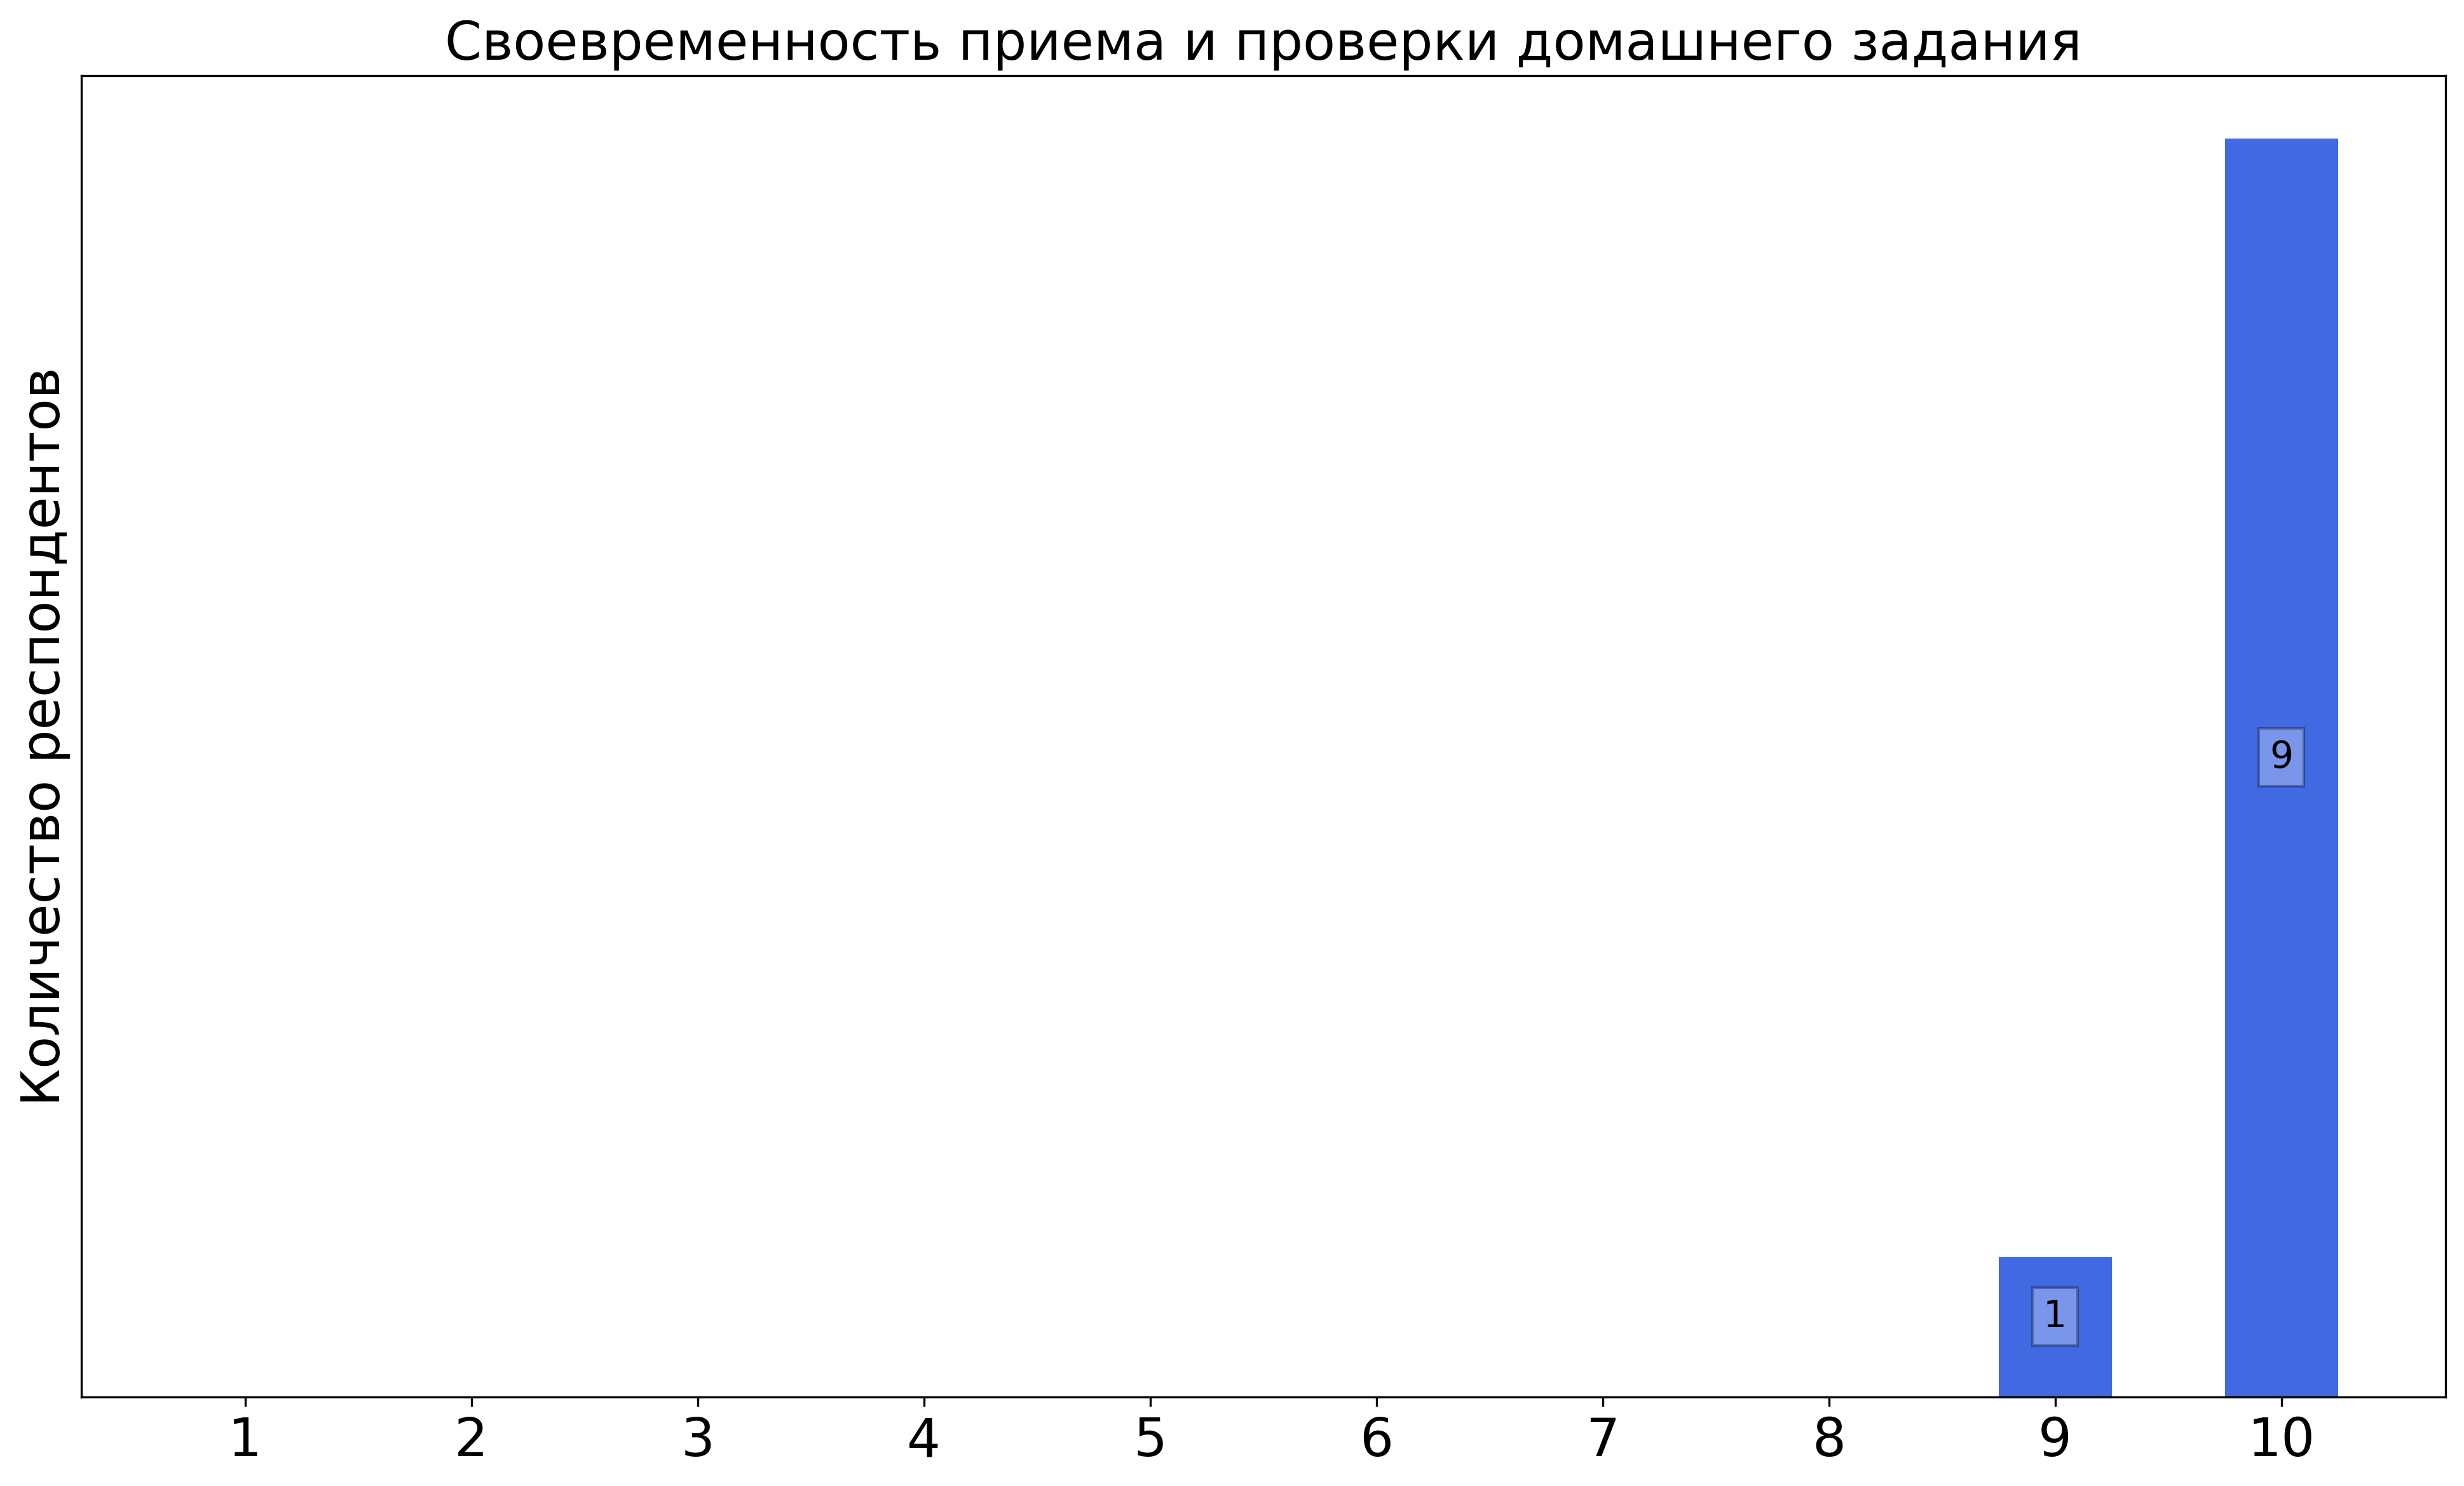
\includegraphics[width=\textwidth]{images/1 course/Математический анализ/seminarists-marks-Кондрашов О.В.-2.png}
			\end{subfigure}
			\begin{subfigure}[b]{0.45\textwidth}
				\centering
				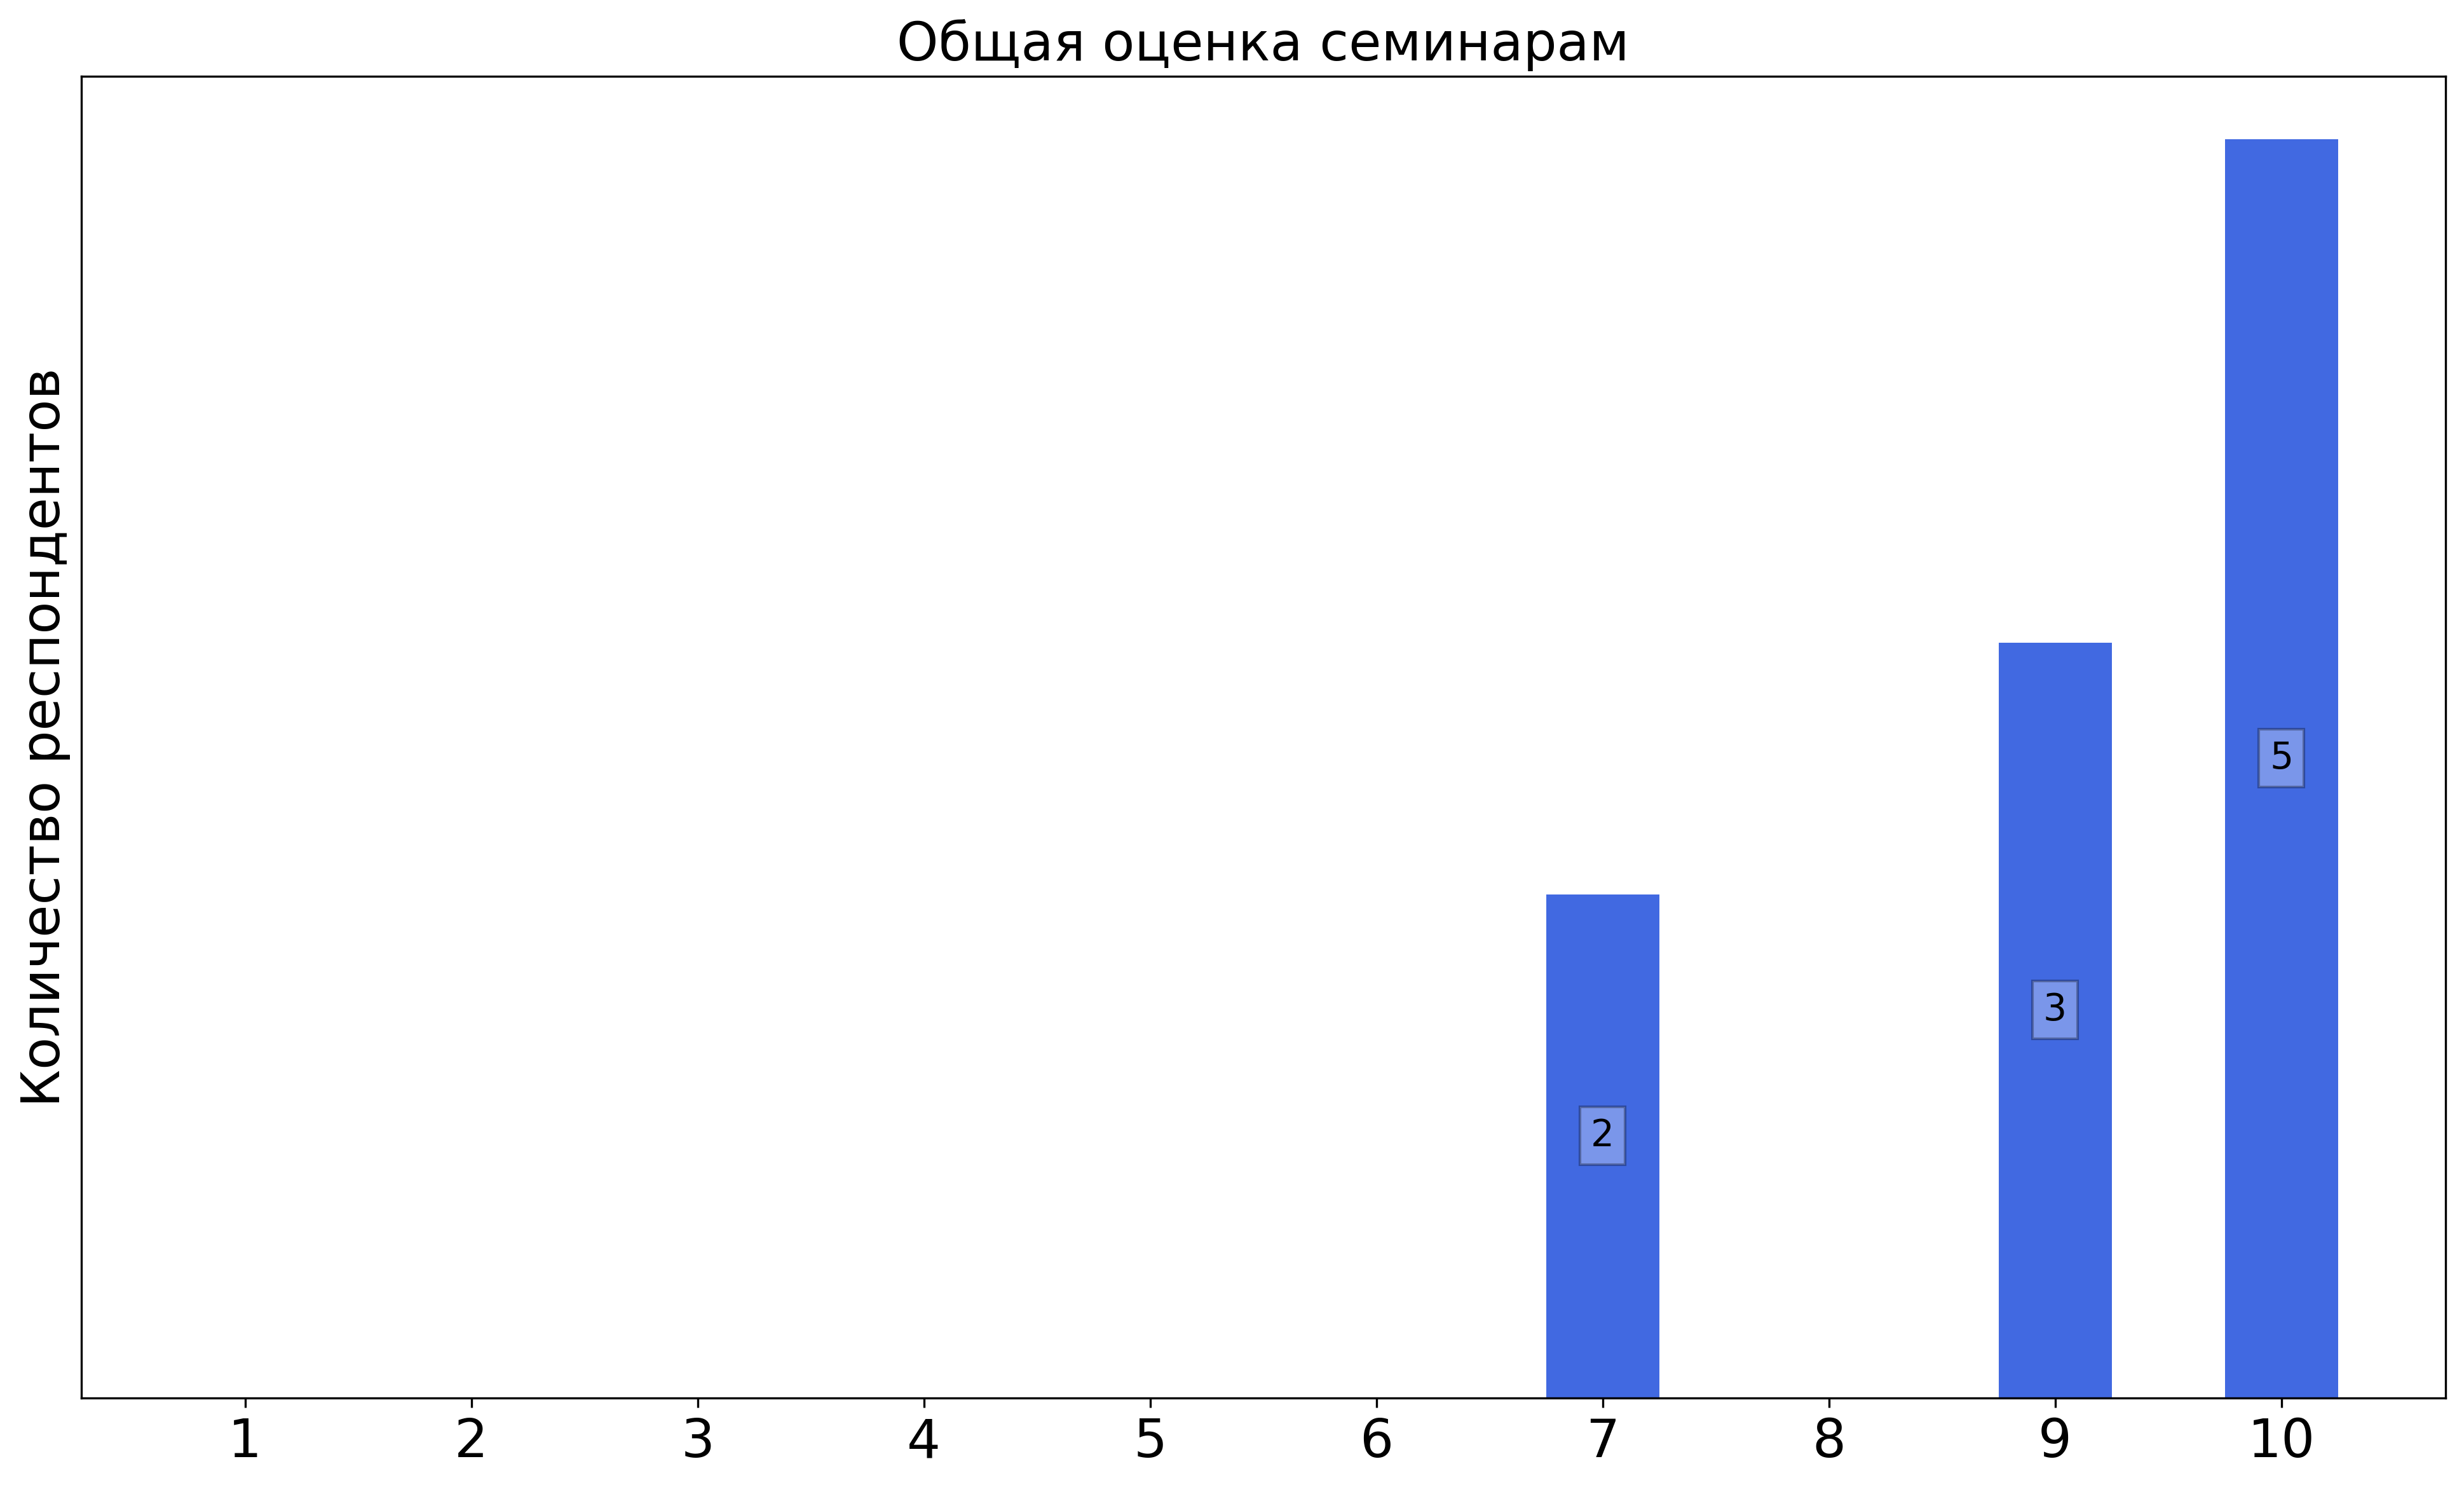
\includegraphics[width=\textwidth]{images/1 course/Математический анализ/seminarists-marks-Кондрашов О.В.-3.png}
			\end{subfigure}	
			\caption{Оценки респондентов о качестве преподавания семинаров}
		\end{figure}

		\textbf{Комментарии студентов о семинаристе\protect\footnote{сохранены оригинальные орфография и пунктуация}}
			\begin{commentbox} 
				Насыщенные, довольно быстрые, даёт материал сразу в общих формулировках, однако пока не могу сказать, это плюс или минус. С одной стороны это сразу целую картину должно создавать, с другой формулировки могут кардинально отличаться от лекционных (и как следствие доказательства тоже могут отличаться) 
			\end{commentbox} 
		
			\begin{commentbox} 
				Очень умный наш Кондрашев, но порой не успеваешь за ним, причем сильно. Приходится самому набирать. Но это физтех, так что не жалуемся  
			\end{commentbox} 
		
			\begin{commentbox} 
				Заставляет делать задачи со звёздочкой 
			\end{commentbox} 
		
			\begin{commentbox} 
				Олег Васильевич - ну просто легендарный семинарист! Его инициативность, системы сдач по теорминимуму Ландау, семинары "в темпе вальса" по-настоящему мотивируют к изучению матанализа 
			\end{commentbox} 

	\subsubsection{Отзыв студентов о семинарах. Семинарист: Шамин А.Ю.}
		\begin{figure}[H]
			\centering
			\begin{subfigure}[b]{0.45\textwidth}
				\centering
				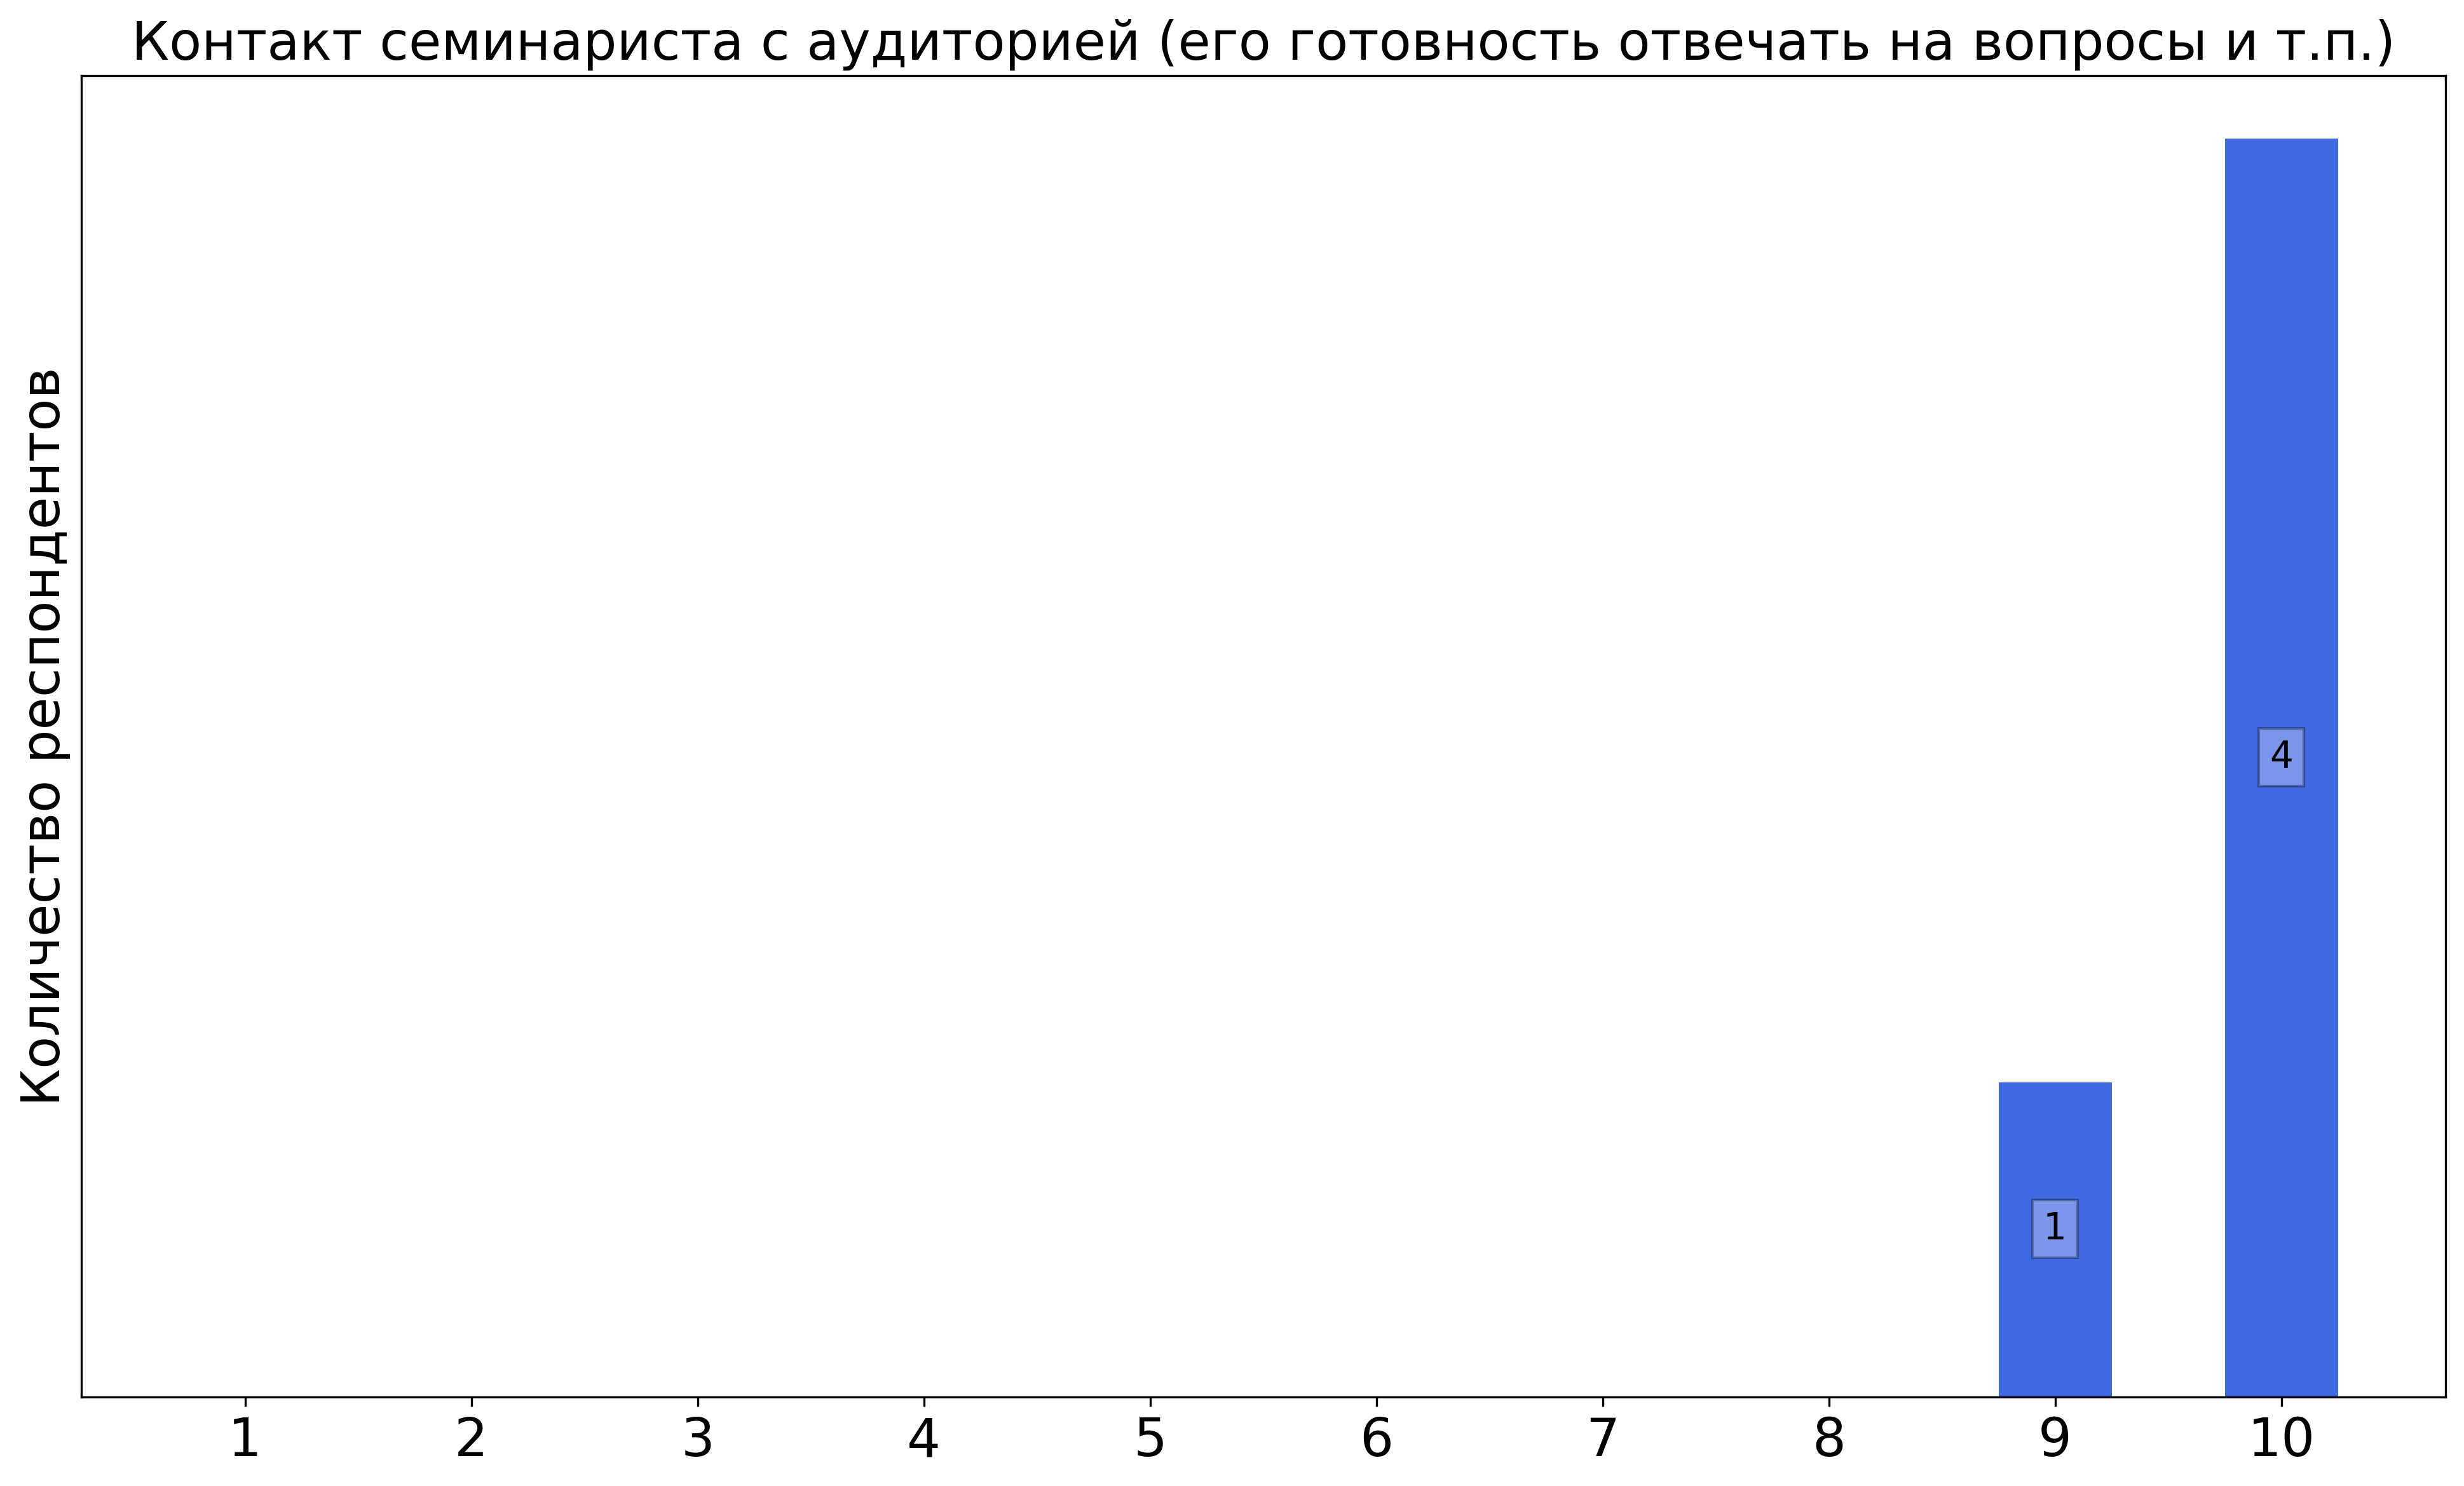
\includegraphics[width=\textwidth]{images/1 course/Математический анализ/seminarists-marks-Шамин А.Ю.-0.png}
			\end{subfigure}
			\begin{subfigure}[b]{0.45\textwidth}
				\centering
				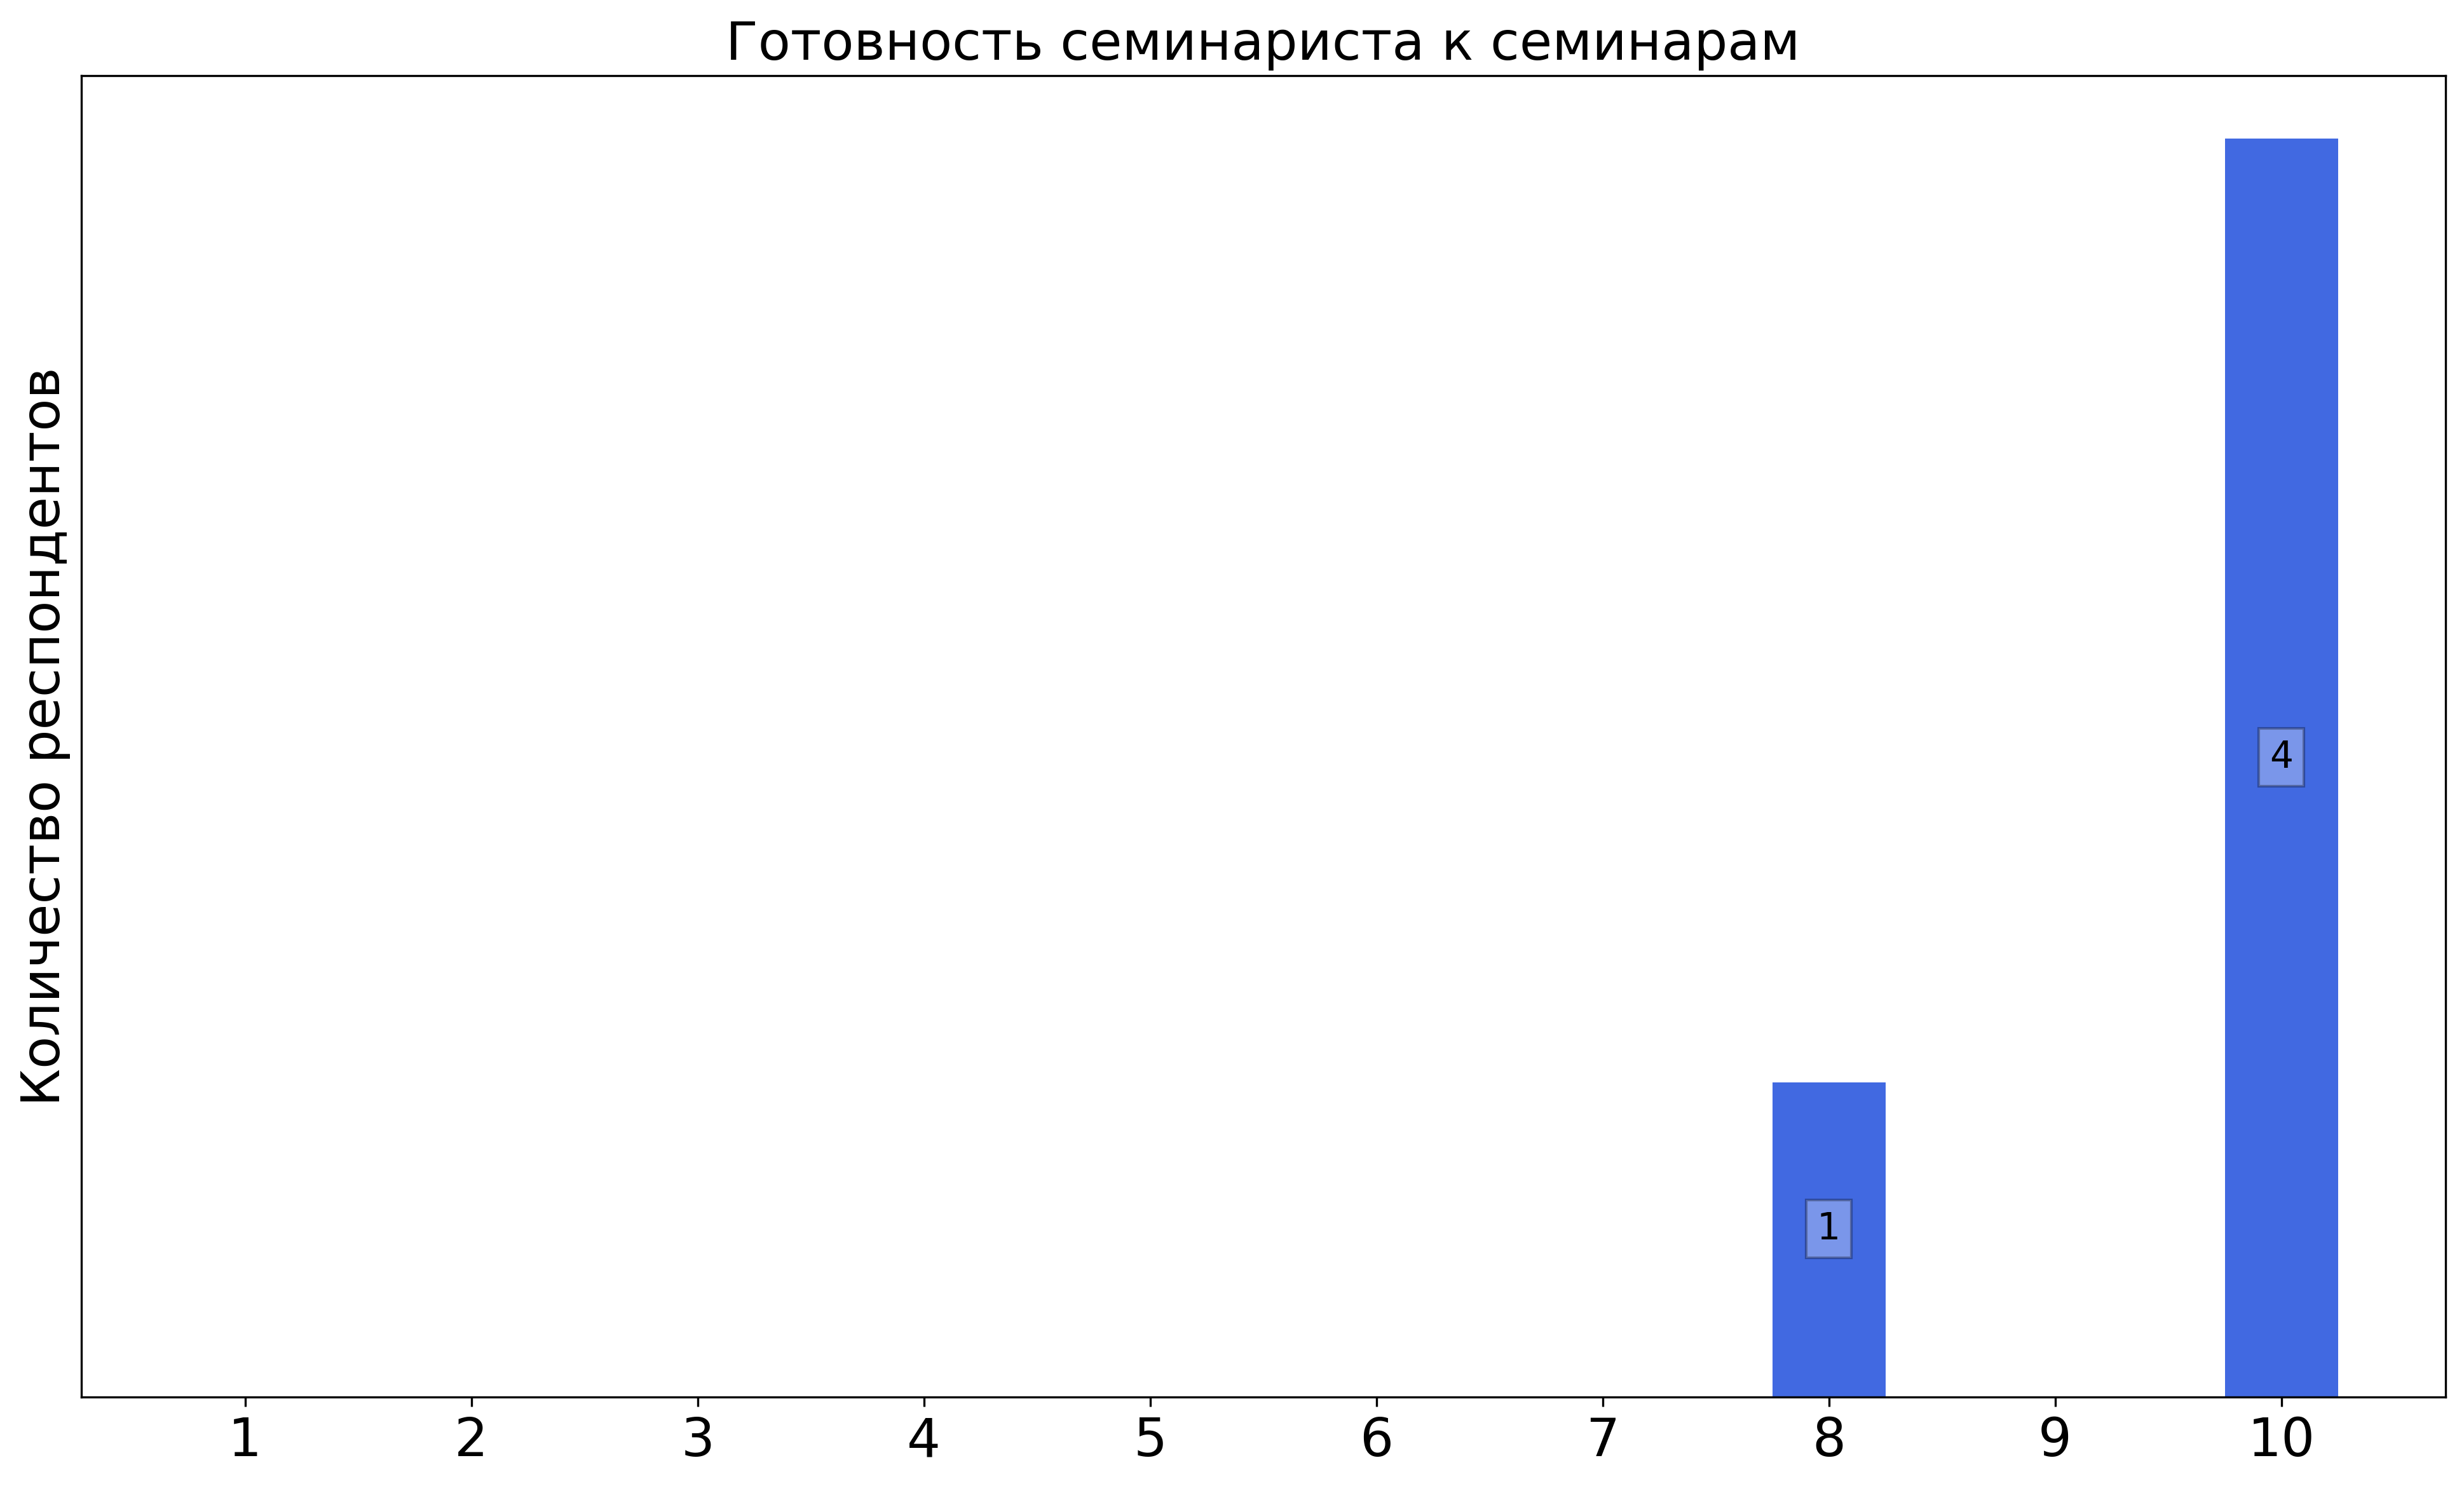
\includegraphics[width=\textwidth]{images/1 course/Математический анализ/seminarists-marks-Шамин А.Ю.-1.png}
			\end{subfigure}
			\begin{subfigure}[b]{0.45\textwidth}
				\centering
				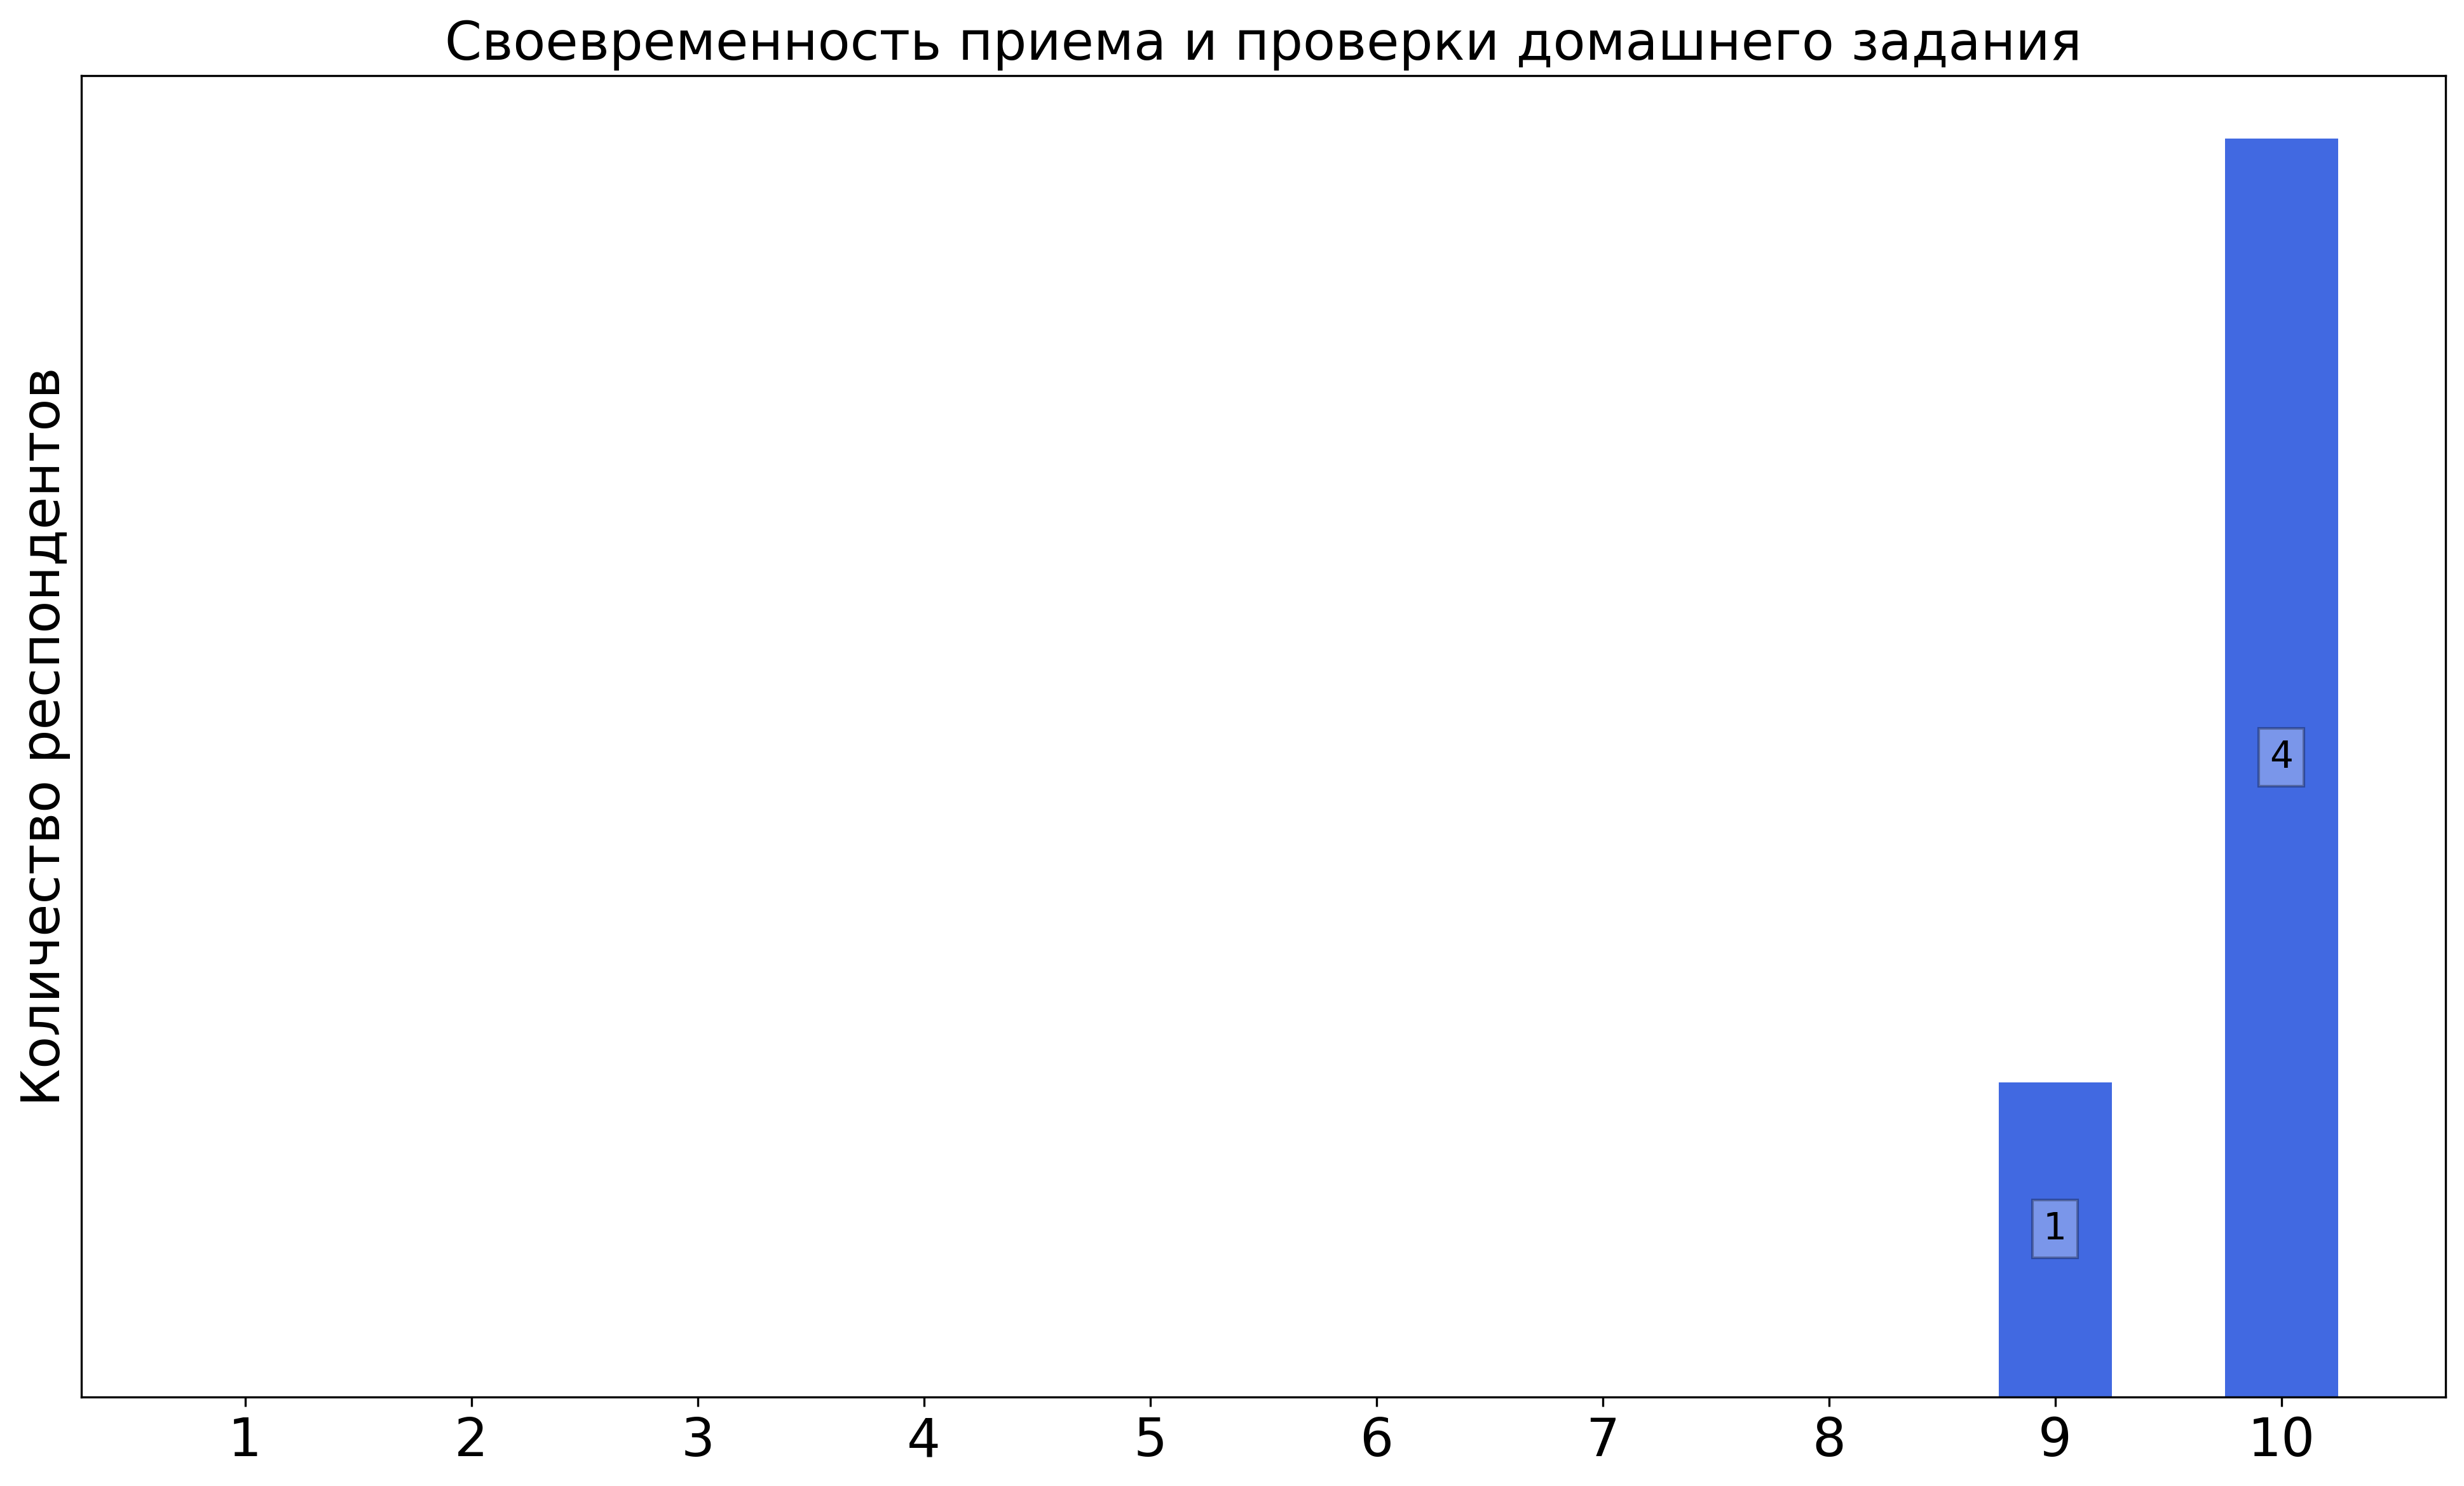
\includegraphics[width=\textwidth]{images/1 course/Математический анализ/seminarists-marks-Шамин А.Ю.-2.png}
			\end{subfigure}
			\begin{subfigure}[b]{0.45\textwidth}
				\centering
				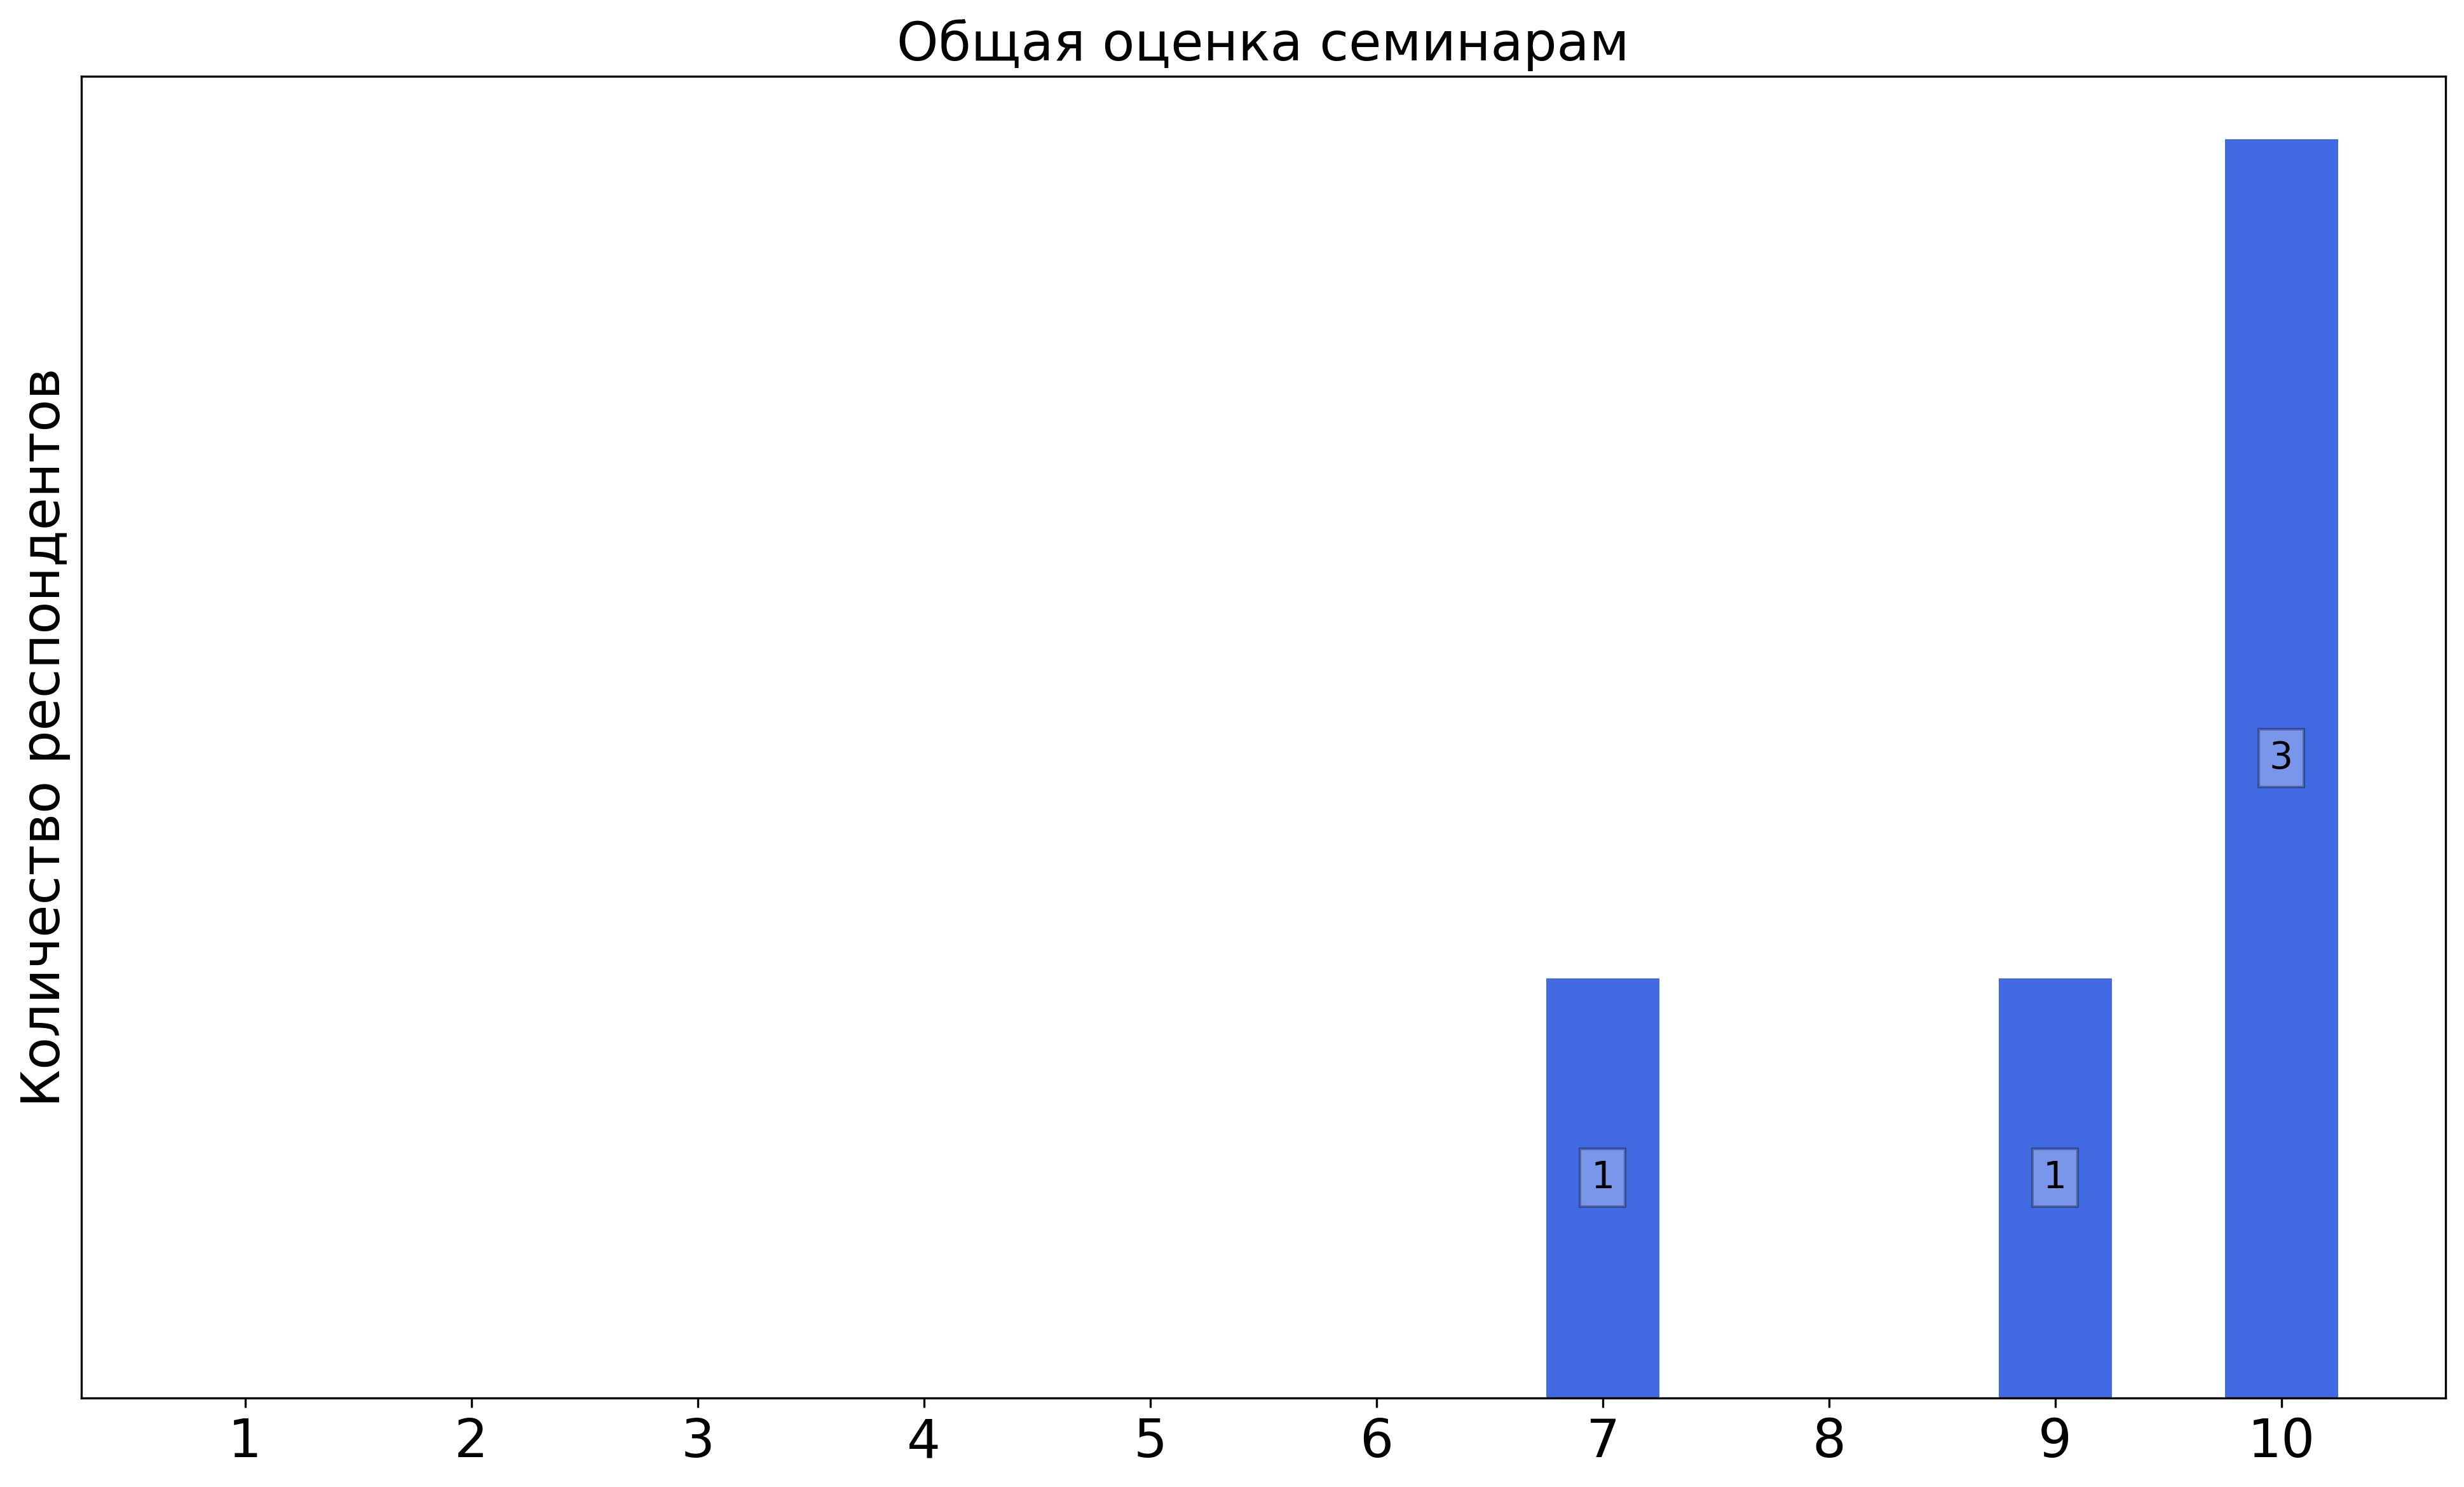
\includegraphics[width=\textwidth]{images/1 course/Математический анализ/seminarists-marks-Шамин А.Ю.-3.png}
			\end{subfigure}	
			\caption{Оценки респондентов о качестве преподавания семинаров}
		\end{figure}

		\textbf{Комментарии студентов о семинаристе\protect\footnote{сохранены оригинальные орфография и пунктуация}}
			\begin{commentbox} 
				Замечательный преподаватель! Объясняет достаточно быстро, но при этом очень понятно. Если ходить на семинары, делать домашнее задание и хорошо заниматься в течение семестра, баллом точно не обидит. Всегда готов идти навстречу студенту, чтобы поднять оценку. 
			\end{commentbox}

	\subsubsection{Прочие комментарии и предложения по улучшению курса}
		\begin{commentbox}
			Домашнее задание на тему интегралов в начале курса очень сильно отвлекает от освоения основного материала
		\end{commentbox}
		
		\begin{commentbox}
			Полное понимание приходит после посещения дополнительных семинаров Скубачевского и общения с однокурсниками. Но лекции отличные
		\end{commentbox}

		\begin{commentbox}
			Круто было бы увидеть учебник Знаменской по второму семестру
		\end{commentbox}

		\begin{commentbox}
			Хотелось бы побольше примеров применения на лекциях, хотя наверное для этого есть семинары
		\end{commentbox}

		\begin{commentbox}
			Наличие книжки, дублирующей лекции оказалось очень удобным. Очень хотелось бы иметь такую в каждом семестре
		\end{commentbox}

		\begin{commentbox}
			Да, в целом, все неплохо, только хотелось бы, чтобы в конце семестра не было прохождения второго семестра
		\end{commentbox}